\appendix
%\addtocontents{toc}{\protect\setlength{\cftsecnumwidth}{7.5em}}%
%\protect\renewcommand*{\protect\cftsecpresnum}{APPENDIX }%

%\include{chapter-appendix}

\begingroup
\clearpage% Manually insert \clearpage
\let\clearpage\relax% Remove \clearpage functionality
\vspace*{-16pt}% Insert needed vertical retraction
\chapter*{\centerline{APPENDICES}}
\addcontentsline{toc}{chapter}{APPENDICES}
\endgroup

% \begin{center}
% {\bfseries Title of Appendix (Not Numbered)}
% \end{center}

\renewcommand{\thesection}{APPENDIX \Alph{section}:}
\addtocontents{toc}{\setlength{\cftsecnumwidth}{16ex}}
%\addtocontents{toc}{%
  %\renewcommand*\cftsecnumwidth{7.4em}%
%  \protect\setlength{\renewcommand*\cftsecnumwidth}{7.5cm}%
%}

\section{GN1 for Upgrade}
\label{appendix:gn1-upgrade}
%\addcontentsline{toc}{chapter}{GN1 for Upgrade}
\numberwithin{equation}{chapter}
\setcounter{equation}{0}

The \gls{gn1} high-level tagger is the newest and the first of the graph neural network architectures lineage. This tagger was designed and 
studied for Run 2, Run 3, and Run 4 (Upgrade) of the \gls{atlas} detector. This tagger's architecture was briefly described in Section \ref{sec:gn1}.
The input variables for this tagger can be seen in Table \ref{tab:gn1-var}. An even newer version of \gls{gn1} tagger has been developed and 
currently being studied for its correlated scale factors that utilizes auxiliary tasks. This newer version is called the GN2 tagger. 
\par
The \gls{gn1} tagger was studied using the same Upgrade samples listed in Table \ref{tab:dl1-samples} and had its performance comapred to 
the DL1d tagger that was trained for this thesis that can be found in Chapter \ref{ch5}. The following 
plots show the performance of the \gls{gn1} tagger to the DL1d and MV2 high-level taggers. The top plots show c-jet rejection and ligh-jet rejection 
using the $t\bar{t}$ sample from Table \ref{tab:dl1-samples}. The middle plots show all three taggers performances using the $\textrm{Z}'$
samples. The results show the clear superiority using the graph neural networks, increasing b-tagging performance 
within c-jet background and light-jet background of up to $~$2.5x. The last two plots show the performances on jetes 
with the new eta range that is available from the \gls{itk} detector. Again, the \gls{gn1} tagger massively 
outperforms the DL1d and MV2 taggers.
\newpage
\begin{figure}[H]
    \centering
    \subfloat[\centering ]{{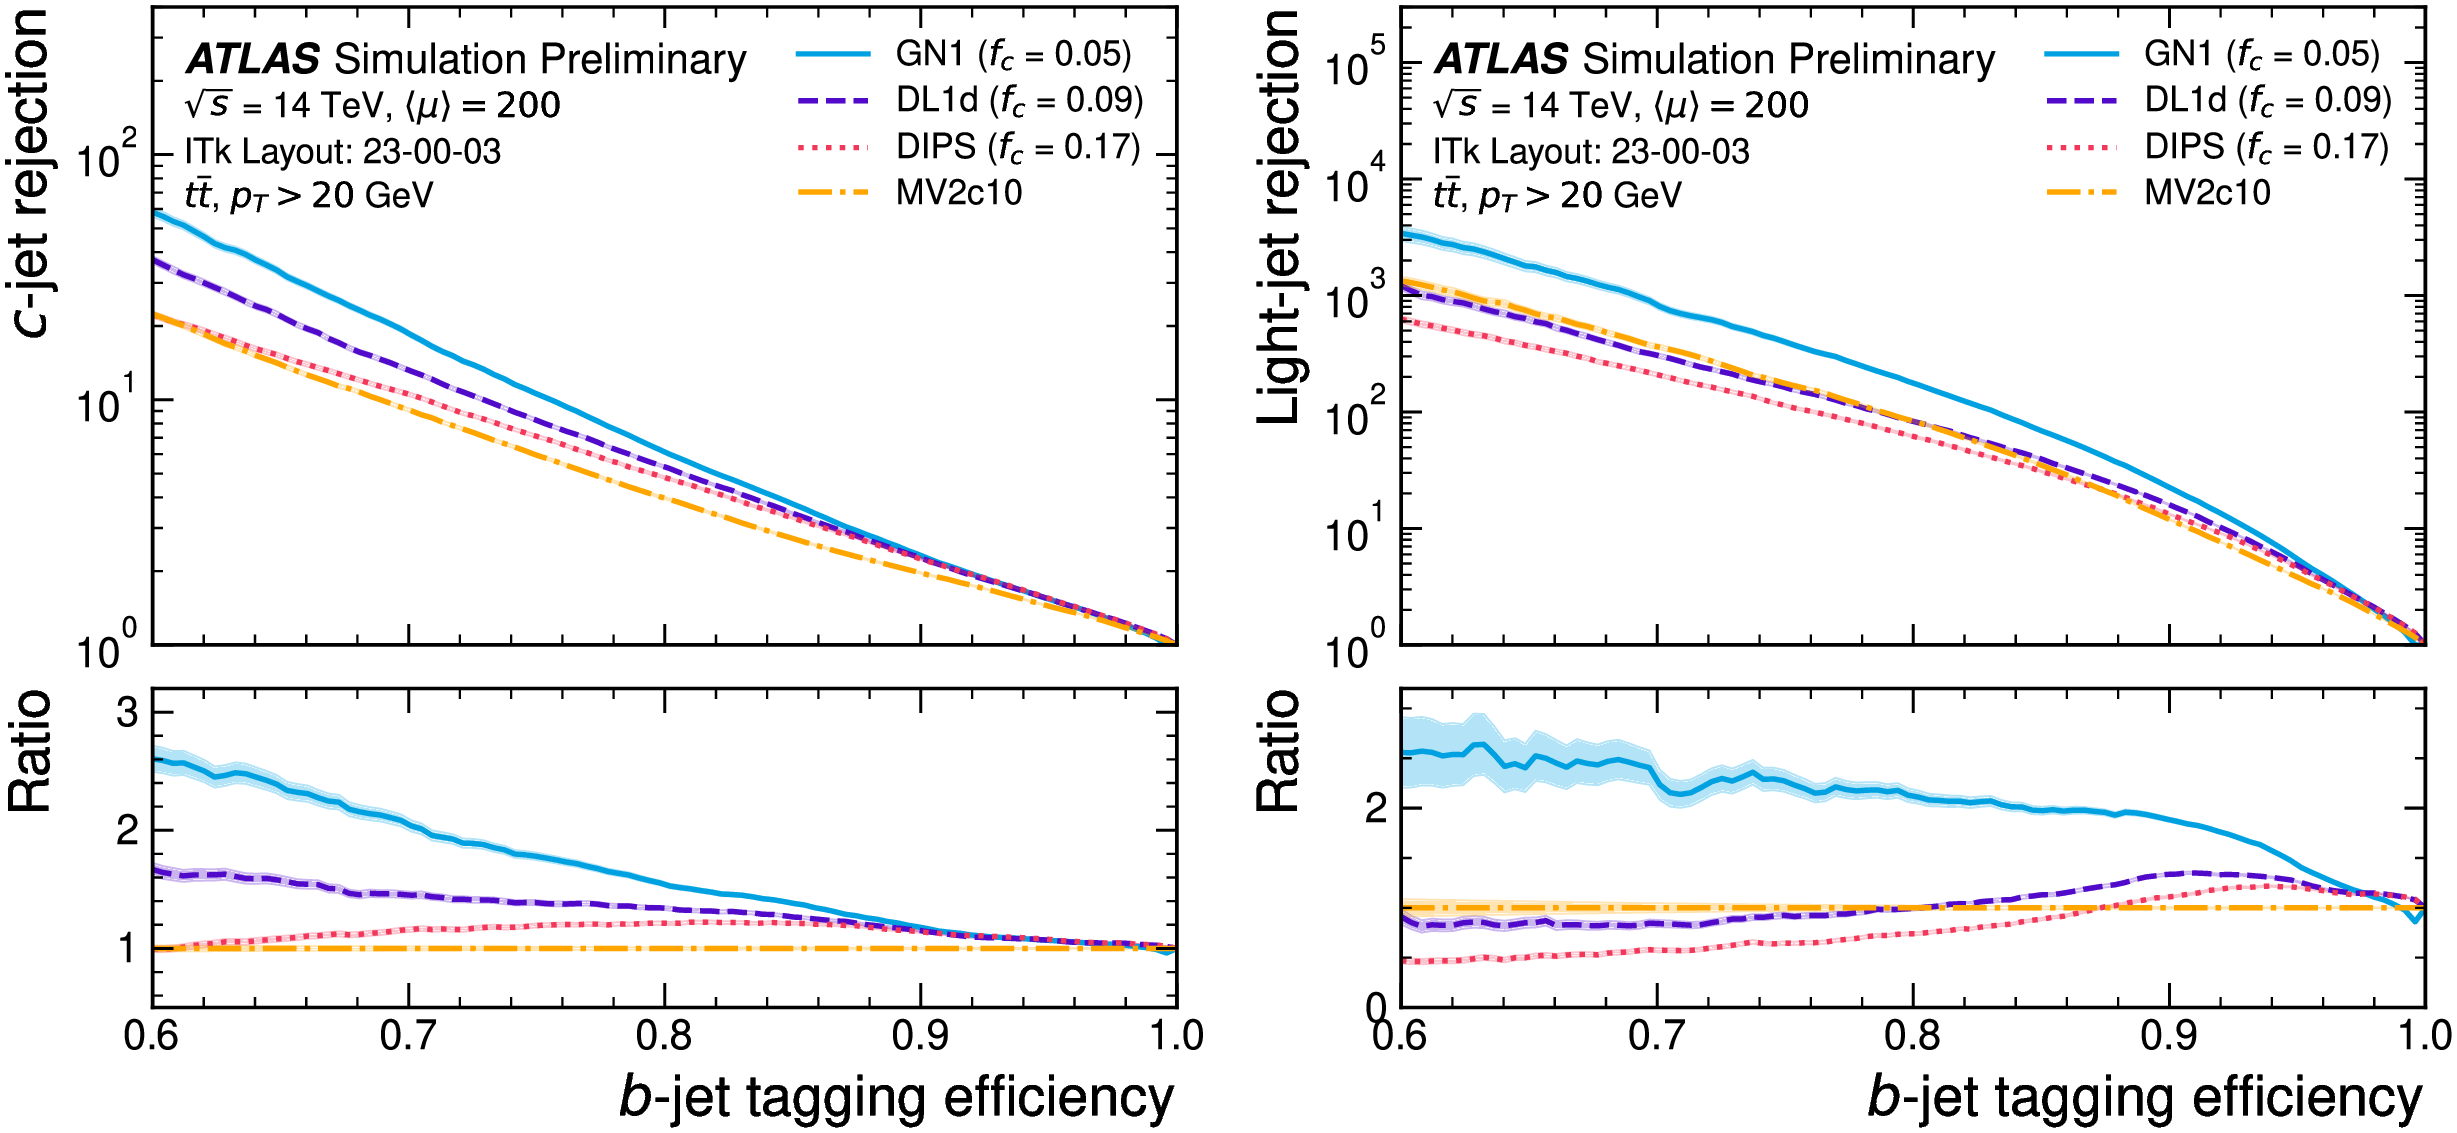
\includegraphics[scale=0.15]{figs/app/gn1-comp-ttbar.png}}}%
    \qquad
    \subfloat[\centering ]{{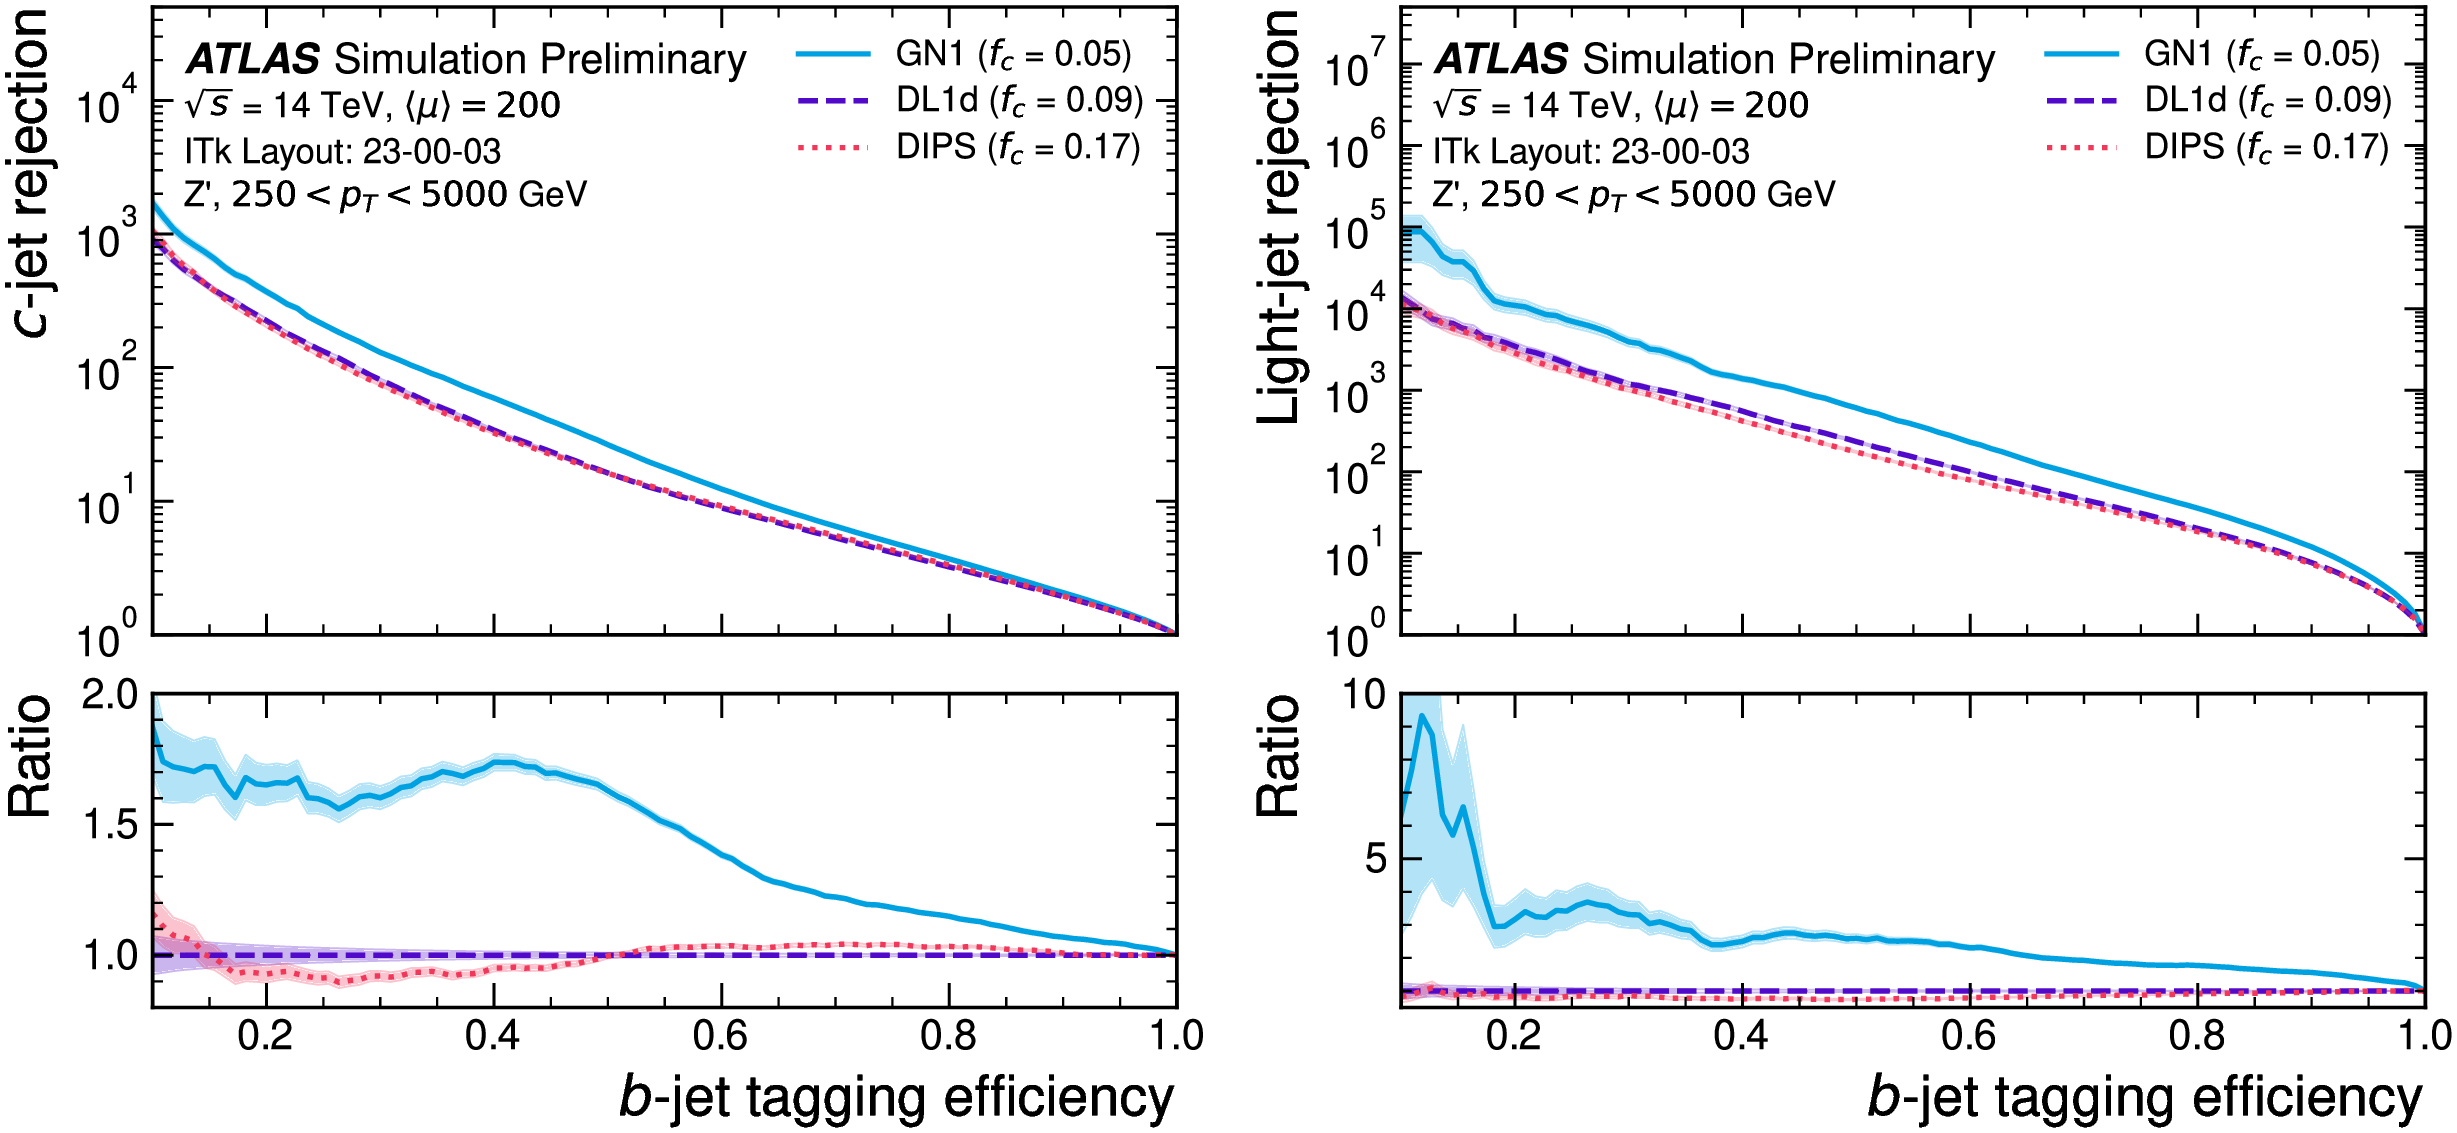
\includegraphics[scale=0.15]{figs/app/gn1-comp-zp.png}}}%
    \qquad
    \subfloat[\centering ]{{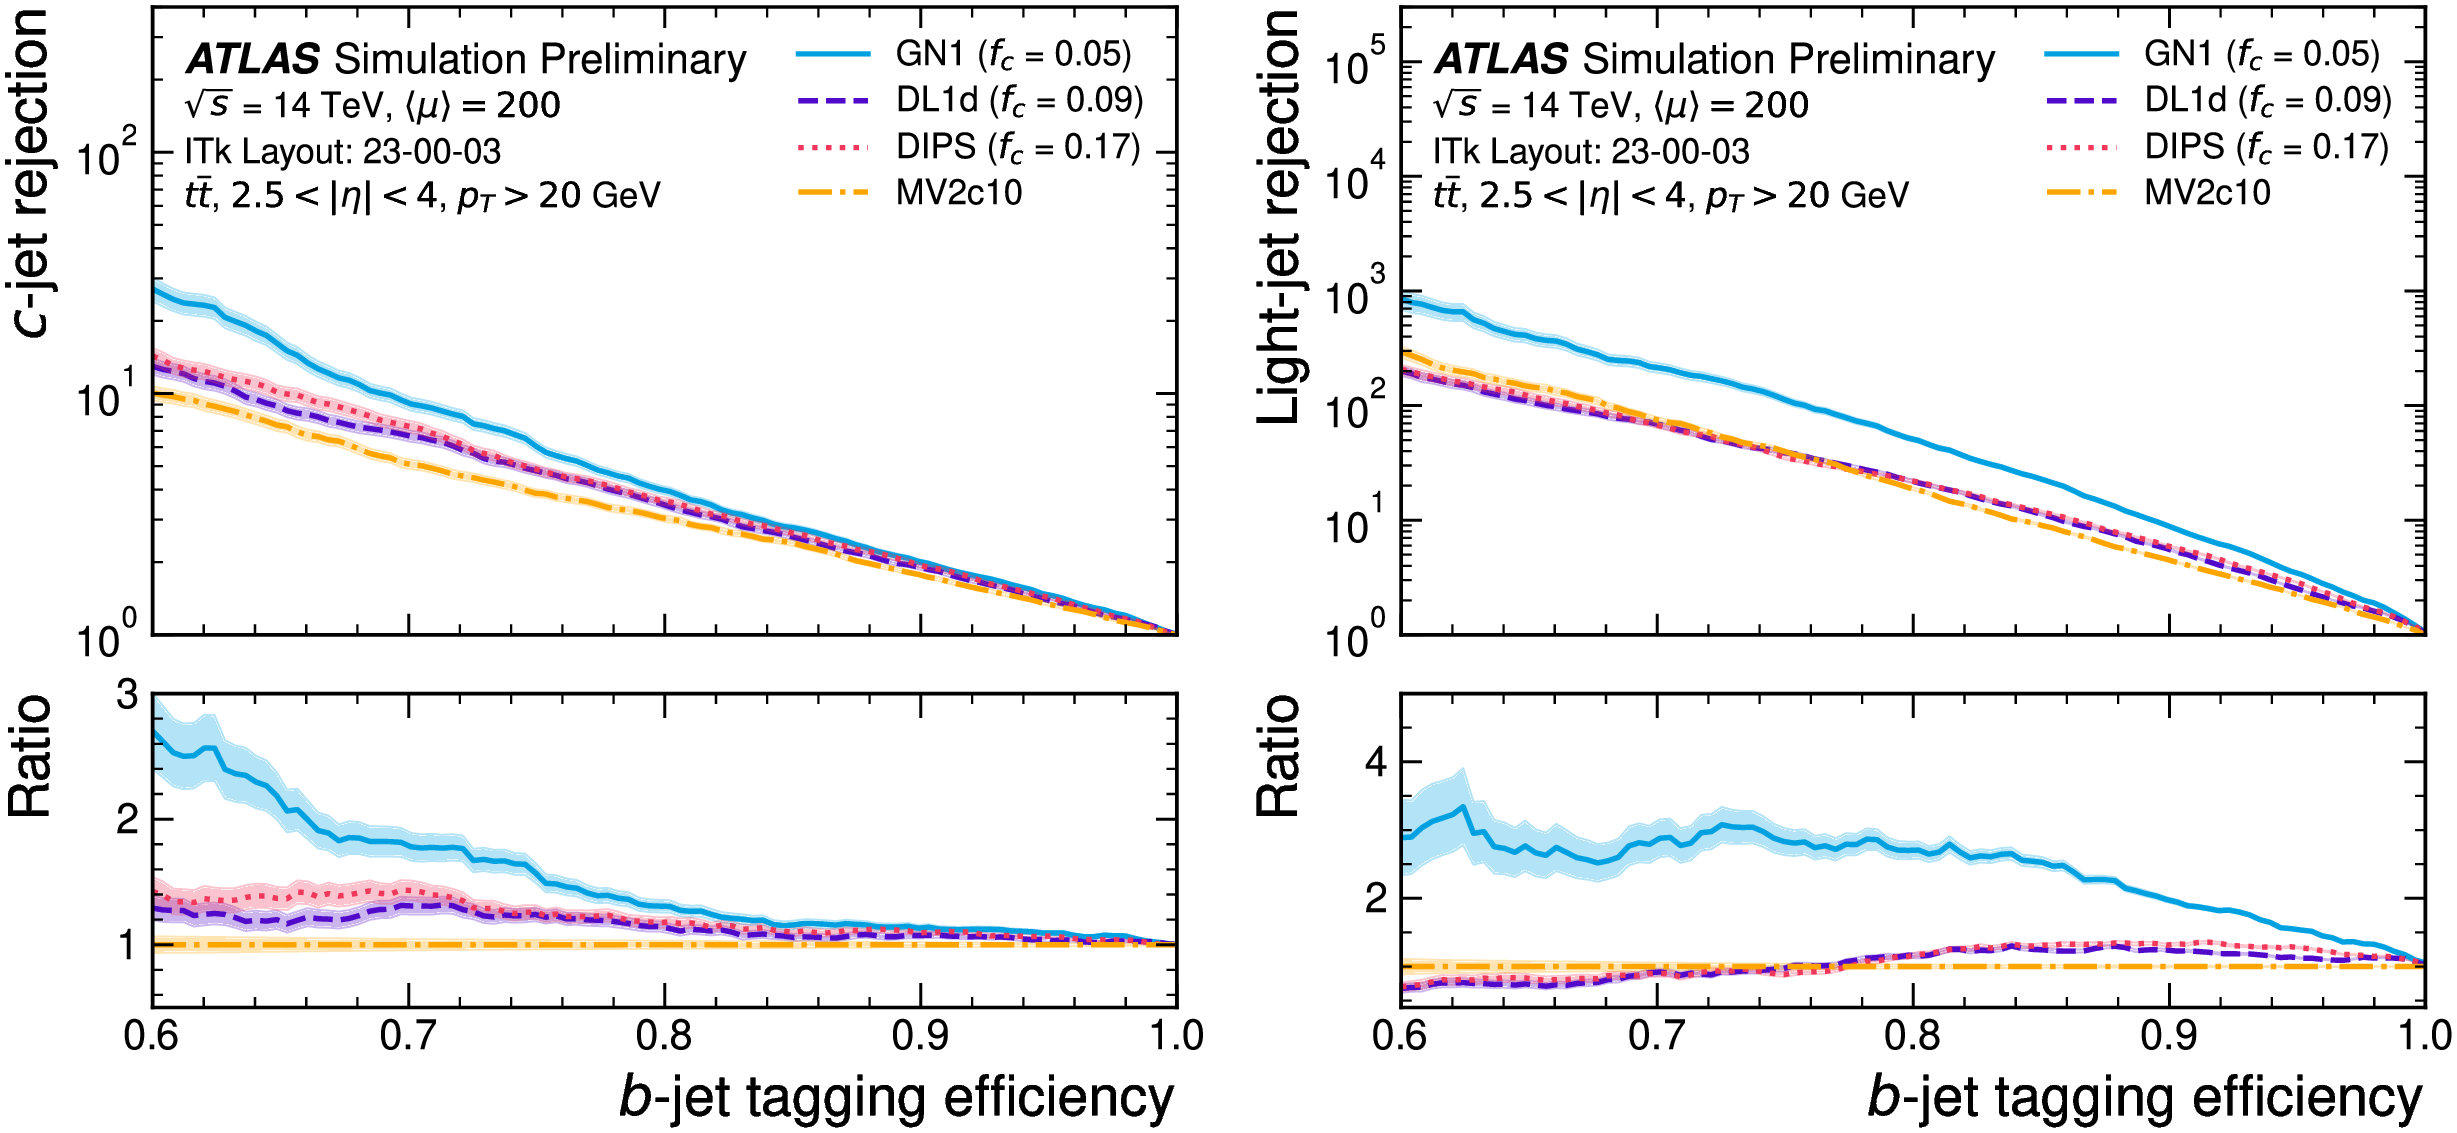
\includegraphics[scale=0.15]{figs/app/gn1-eta.png}}}%
    \caption{ GN1, DL1d and the MV2 high-level tagger performances on the $t\bar{t}$ and $\textrm{Z}'$ samples list in Table \ref{tab:dl1-samples} \cite{dl1d-hllhc-ftag}.}
\label{fig:gn1-perf}
\end{figure}

\newpage
\begin{table}[H]
    \setlength\extrarowheight{-3pt}
    \centering 
    \begin{tabular}{ |m{5cm} |m{12cm} |}
        \hline
        \multicolumn{2}{|c |}{GN1 Input Variables}\\
        \hline\hline
        Jet Input & Description \\
        \hline
        $\textrm{P}_{\textrm{T}}$ & Jet transverse momentum \\ 
        $\textrm{η}$ & Signed jet pseudorapidity \\
        \hline\hline
        Track Input & Description \\
        \hline
         q/$\textrm{\textit{p}}$ & Track charge divided by momentum (measure of curvature) \\
         $\textrm{d}_{\textrm{η}}$ & Pseudorapidity of the track, relative to the jet η \\
         $\textrm{d}_{\phi}$ & Azimuthal angle of the track, relative to the jet $\phi$ \\
         $\textrm{d}_{\textrm{0}}$ & Closest distance from the track to the PV in the longitudinal plane \\
         $\textrm{\textit{z}}_{\textrm{0}}\textrm{sin}\theta$ & Closest distance from the track to the PV in the transverse plane \\
         $\sigma(q/\textrm{\textit{p}})$ & Uncertainty on q/$\textrm{\textit{p}}$\\
         $\sigma(\theta)$ & Uncertainty on track polar angle $\theta$\\
         $\sigma(\phi)$ & Uncertainty on track azimuthal angle $\phi$ \\
         s($\textrm{d}_{\textrm{0}}$) & Lifetime signed transverse IP significance\\
         s($\textrm{\textit{z}}_{\textrm{0}}\textrm{sin}\theta$) & Lifetime signed longitudinal IP significance\\
         nPixHits & Number of pixel hits \\
         nStripHits & Number of strip hits \\
         nInnermostPixHits & Number of hits from the innermost pixel layer \\
         nNextToInndermostPixHits & Number of hits from the next-to-innermost pixel layer \\
         nInnermostPixShared & Number of shared hits from the innermost pixel layer \\
         nInnermostPixSplit & Number of split hits from the innermost pixel layer \\
         nPixShared & Number of shared pixel hits \\
         nPixSplit & Number of split pixel hits \\
         nStripShared & Number of shared strip hits \\
         nPixHoles & Number of pixel holes \\
         nStripHoles & Number of strip holes \\
         \hline
    \end{tabular}\hfill
    \caption{ Input features to the GN1 model. Basic jet kinematics, along with information about the reconstructed track parameters and constituent hits are used \cite{dl1d-hllhc-ftag}.}
    \label{tab:gn1-var}
\end{table}

\newpage

\vspace*{0.6in}

\section{Run2 Datasets and HLT Lepton Triggers for Anomaly Detection}
\label{appendix:hlt-triggers-ad}
%\addcontentsline{toc}{chapter}{Run2 Datasets and HLT Lepton Triggers for Anomaly Detection}
\numberwithin{equation}{chapter}
\setcounter{equation}{0}

All the data used in this analysis is originated from the \gls{atlas} detector during the Run 2 period between the years 2015 to 2018. The dat was recorded during stable beam conditions 
while all relevant subdetectors were fully operational. The event candidates selected was done by either single-electron triggers or single-muon triggers which range in transverse momenta, 
transverse energy, and quality and isolation thresholds. The preselected data derive from the Good Run Lists (\gls{grl}) for 2015-2018 for release 21:
\\
\\
\begin{footnotesize}
\texttt{2015: data15\_13TeV.periodAllYear\_DetStatus-v89-pro21-02\_Unknown\_PHYS\_StandardGRL\_All\_Good\\\_25ns.xml} \\
\\
\texttt{2016: data16\_13TeV.periodAllYear\_DetStatus-v89-pro21-01\_DQDefects-00-02-04\_PHYS\_\\StandardGRL\_All\_Good\_25ns.xml} \\
\\
\texttt{2017: data17\_13TeV.periodAllYear\_DetStatus-v99-pro22-01\_Unknown\_PHYS\_StandardGRL\_All\\\_Good\_25ns\_Triggerno17e33prim.xml} \\
\\
\texttt{2018: data18\_13TeV.periodAllYear\_DetStatus-v102-pro22-04\_Unknown\_PHYS\_StandardGRL\_All\\\_Good\_25ns\_Triggerno17e33prim.xml}\\
\end{footnotesize}
\\
The files process from these \gls{grl} lists come in a format called DAOD\_STDM4 and required at least one lepton \gls{hlt} trigger for either electron or muon \gls{hlt}s. All saved objects 
within these files required at least a transverse momenta above 20 GeV for further preselection. The datasets in this STDM4 derivation format used for this analysis are:
\\
\\
\begin{footnotesize}
\texttt{data15\_13TeV.period[D-J].physics\_Main.PhysCont.DAOD\_STDM4.grp23\_v01\_p4238} \\
\texttt{data16\_13TeV.period[A-G,I,K,L].physics\_Main.PhysCont.DAOD\_STDM4.grp23\_v01\_p4238} \\
\texttt{data17\_13TeV.period[B-F,H,I,K].physics\_Main.PhysCont.DAOD\_STDM4.grp23\_v01\_p4238} \\
\texttt{data18\_13TeV.period[B-D,F,I,K-M,O,Q].physics\_Main.PhysCont.DAOD\_STDM4.grp23\_v01\_p4238} \\
\end{footnotesize}
\\
Mini-trees were created from these dataset containers using the framework xAODAnaHelpers (AnalysisBase,21.2.177) and the Wjet framework that was developed in release 21.2.177, selecting 
events with leptons that pass the \gls{hlt} triggers. The triggers in which dominate consistent efficiency over the data-taking period are the single lepton triggers with $\textrm{P}_{\textrm{T}}^{\textrm{l}} \ >$  60 GeV.
The naming convention for these triggers follows \texttt{HLT\_muNN[\_isoInfo]}, where \texttt{NN} specifies the $\textrm{P}_{\textrm{T}}$ threshold and the \texttt{isInfo} is the isolation requirement.
Similarly for electron, the trigger naming convention is such \texttt{HLT\_eNN\_IDinfo[\_lhInfo][\_isoInfo]} where the \texttt[IDinfo] is the information on the identification requirement,
\texttt{lhInfo} is an option requirement that enters the identification likelihood calculation and the \texttt{isoInfo} is the isolation requirement. 
The \gls{hlt} triggers used in this analysis for both electron and muons are as following:
\\
\\
\textbf{Muon Triggers}
\\
\begin{small}
\texttt{HLT\_mu24\_iloose     ||  HLT\_mu24ivarloose    ||  HLT\_24ivarmedium   ||} \\
\texttt{HLT\_mu26\_ivarmedium ||  HLT\_mu24imedium      ||  HLT\_mu26\_imedium HLT\_mu40  || HLT\_mu50}\\
\\
\end{small}
\textbf{Electron Triggers}
\\
\begin{small}
\texttt{HLT\_e26\_lhtight\_nod0\_ivarloose    ||  HLT\_e24\_lhmedium\_nod0\_iverloose  ||}\\
\texttt{HLT\_e60\_medium                      ||  HLT\_e60\_lhmedium\_nod60}\\
\end{small}

\newpage

\vspace*{0.5in}

\section{Monte Carlo Samples for the Background Hypothesis}
\label{appendix:mc-ad}
%\addcontentsline{toc}{chapter}{Monte Carlo Samples for the Background Hypothsis}
\numberwithin{equation}{chapter}
\setcounter{equation}{0}

The dominant source of background samples used for this analysis are $t\bar{t}$ and signle-top events along with W+jets simulated processes. Multi-jet processes are estimated using a loose 
lepton control region from data. The $t\bar{t}$ events are from the sample:
\\
{\footnotesize \texttt{mc16\_13TeV.410470.PhPy8EG\_A14\_ttbar\_hdamp258p75\_nonallhad.deriv.DAOD\_STDM4.\%p4237}}
\\
After requiring at least one lepton above 60 GeV, 25M events were left. 
\\
The single top samples used were:
\\
\\
\begin{footnotesize}
\texttt{mc16\_13TeV.410644.PowhegPythia8EvtGen\_A14\_singletop\_\%.DAOD\_STDM4.\%p4237}\\
\texttt{mc16\_13TeV.410646.PowhegPythia8EvtGen\_A14\_Wt\_DR\_inclusive\_top.\%.DAOD\_STDM4.\%p4237}\\
\texttt{mc16\_13TeV.410647.PowhegPythia8EvtGen\_A14\_Wt\_DR\_inclusive\_antitop.\%.DAOD\_STDM4.\%p4237}\\
\texttt{mc16\_13TeV.410658.PhPy8EG\_A14\_tchan\_BW50\_lept\_top.deriv.DAOD\_STDM4.\%p4237}\\
\texttt{mc16\_13TeV.410659.PhPy8EG\_A14\_tchan\_BW50\_lept\_antitop.deriv.DAOD\_STDM4.\%p4237}\\
\end{footnotesize}
\\
These include three different processes, single-top, \textit{l}+t, and W+t. All these are considered ``single-top'' processes within this analysis. 
The total amount of events from these datasets after requiring at least one lepton above 60 GeV is about 6M. 
\\
The W+jets samples are: 
\\
\\
\begin{footnotesize}
\texttt{mc16\_13TeV.361100.PowhegPythia8EvtGen\_AZNLOCTEQ6L1\_Wplusenu.deriv.DAOD\_STDM4.\%p4237}\\
\texttt{mc16\_13TeV.361103.PowhegPythia8EvtGen\_AZNLOCTEQ6L1\_Wminusenu.deriv.DAOD\_STDM4.\%p4237}\\
\texttt{mc16\_13TeV.361101.PowhegPythia8EvtGen\_AZNLOCTEQ6L1\_Wplusmunu.deriv.DAOD\_STDM4.\%p4237}\\
\texttt{mc16\_13TeV.361104.PowhegPythia8EvtGen\_AZNLOCTEQ6L1\_Wminusmunu.deriv.DAOD\_STDM4.\%p4237}\\
\end{footnotesize}
\\
After requiring at least one lepton above 60 GeV, these samples contained about 4M events. There are 140M events from the data taken in Run2 within the defined signal region after the 
final selection described in section \ref{sec:final_sel}. The total amount of Monte Carlo simulated events after the final selection is about 14M, so about 10\% of data. Once the 
loose lepton control region is added from the data, this gives sufficient amount of events to conclude a smooth falling background shape. 
These samples were processed using the full \gls{atlas} detector simulation based on Geant4 and the pile-up conditions were matched per data-taking year. 
\newpage

\vspace*{0.6in}

\section{RMM Event Examples}
\label{appendix:rmm-event-examples}
%\addcontentsline{toc}{chapter}{RMM Event Examples}
\numberwithin{equation}{chapter}
\setcounter{equation}{0}

Figure~\ref{fig:rmm-data1} - \ref{fig:rmm_tt5} shows single events converted to \gls{rmm}. The 9 invariant masses of interest are removed.

\begin{figure}[H]
    \begin{center}
        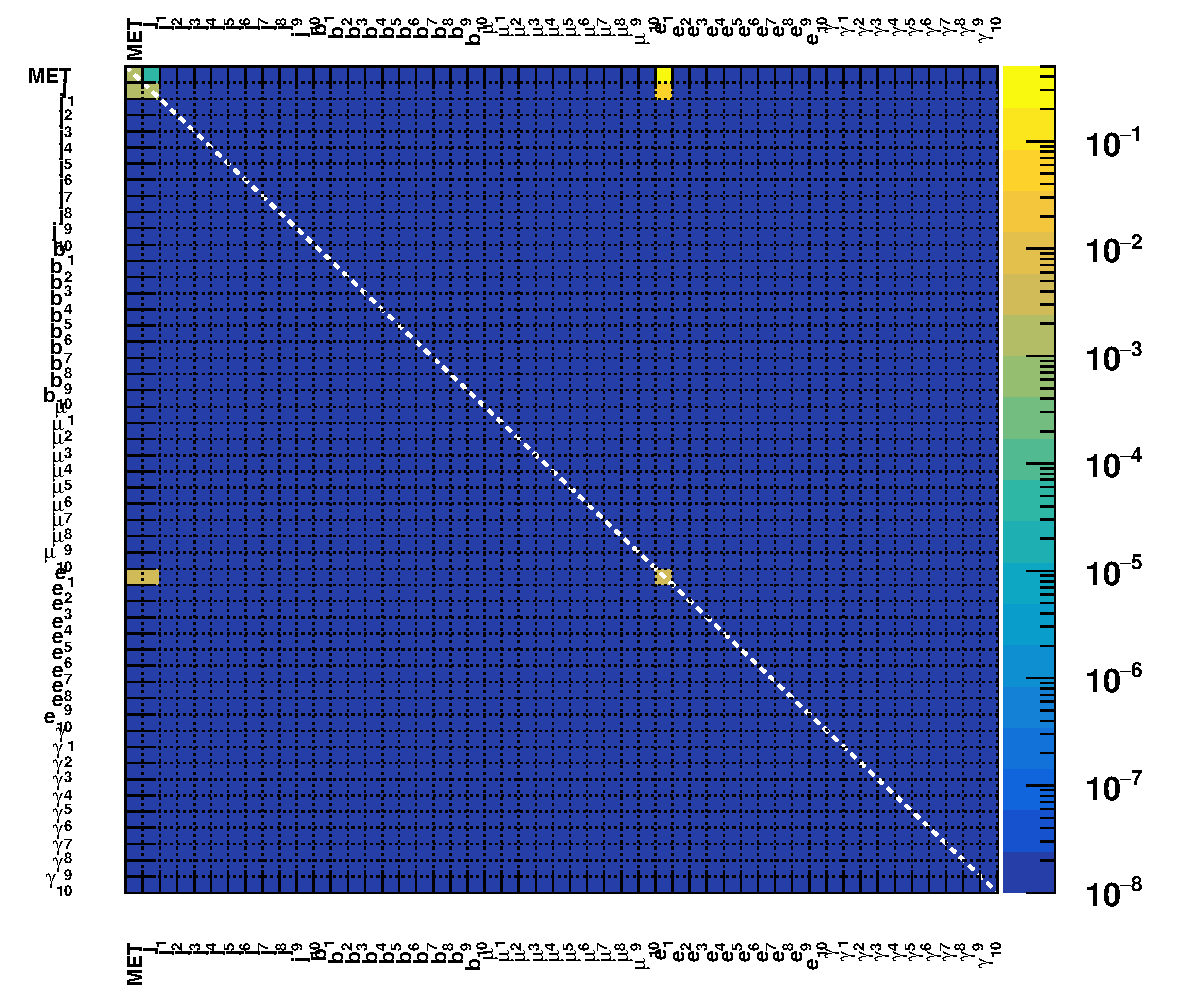
\includegraphics[width=0.9\textwidth]{figs/app/validate_event1_data.pdf}
    \end{center}
    \caption{
    A typical data event (from 2016) shown as RMM.
    The event has one jet, one electron and some (small) MET.
    }
\label{fig:rmm-data1}
\end{figure}

\begin{figure}[H]
    \begin{center}
        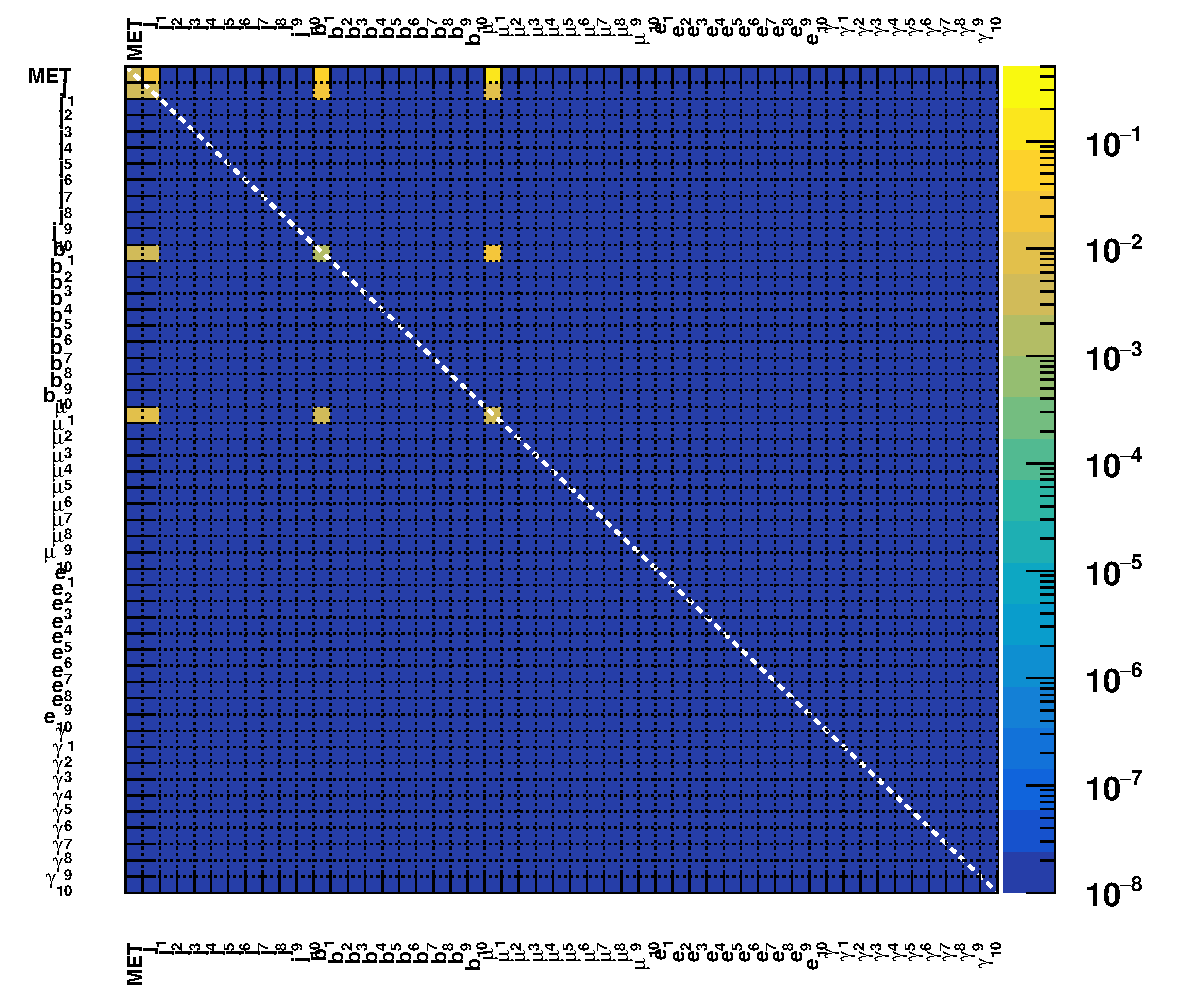
\includegraphics[width=0.9\textwidth]{figs/app/validate_event1_ttbar.pdf}
    \end{center}
    \caption{
    A typical $t\bar{t}$  event from a Monte Carlo simulation.
    The event has one jet, one $b$-jet, one muon and some  MET.
    }
    \label{fig:rmm_tt1}
\end{figure}

\begin{figure}[H]
    \begin{center}
        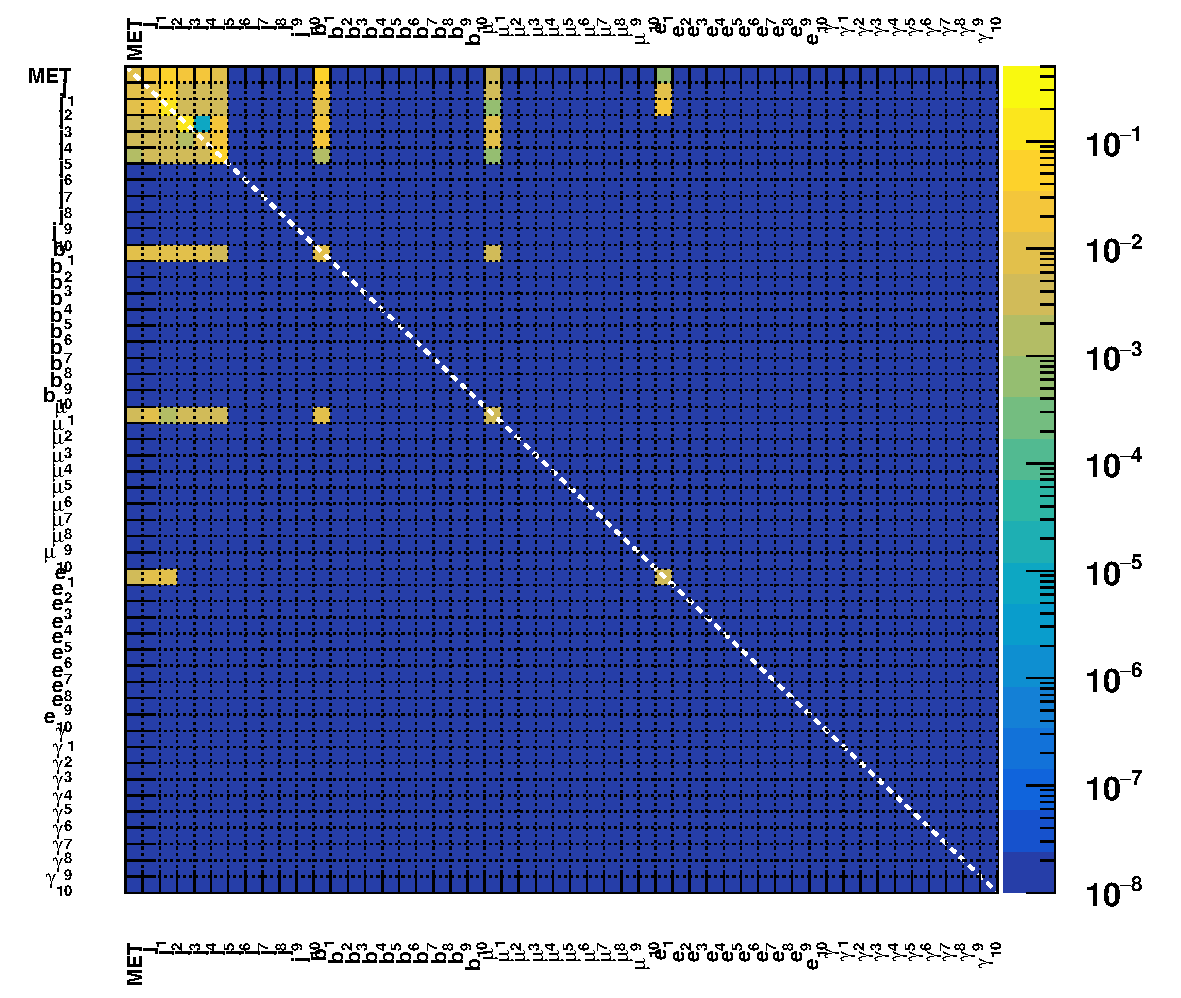
\includegraphics[width=0.9\textwidth]{figs/app/validate_event1_ssm.pdf}
    \end{center}
    \caption{
    A typical the sequential standard model $W'\to W Z' \to l\nu q\bar{q}$  event with $W'$ at 0.75 TeV and $Z'$ at 0.5 TeV 
    decaying to 2 jets, with the leptonic decay of $W$.
    The event has multiple jets, leptons and some  MET.
    }
    \label{fig:rmm_tt2}
\end{figure}

\begin{figure}[H]
    \begin{center}
        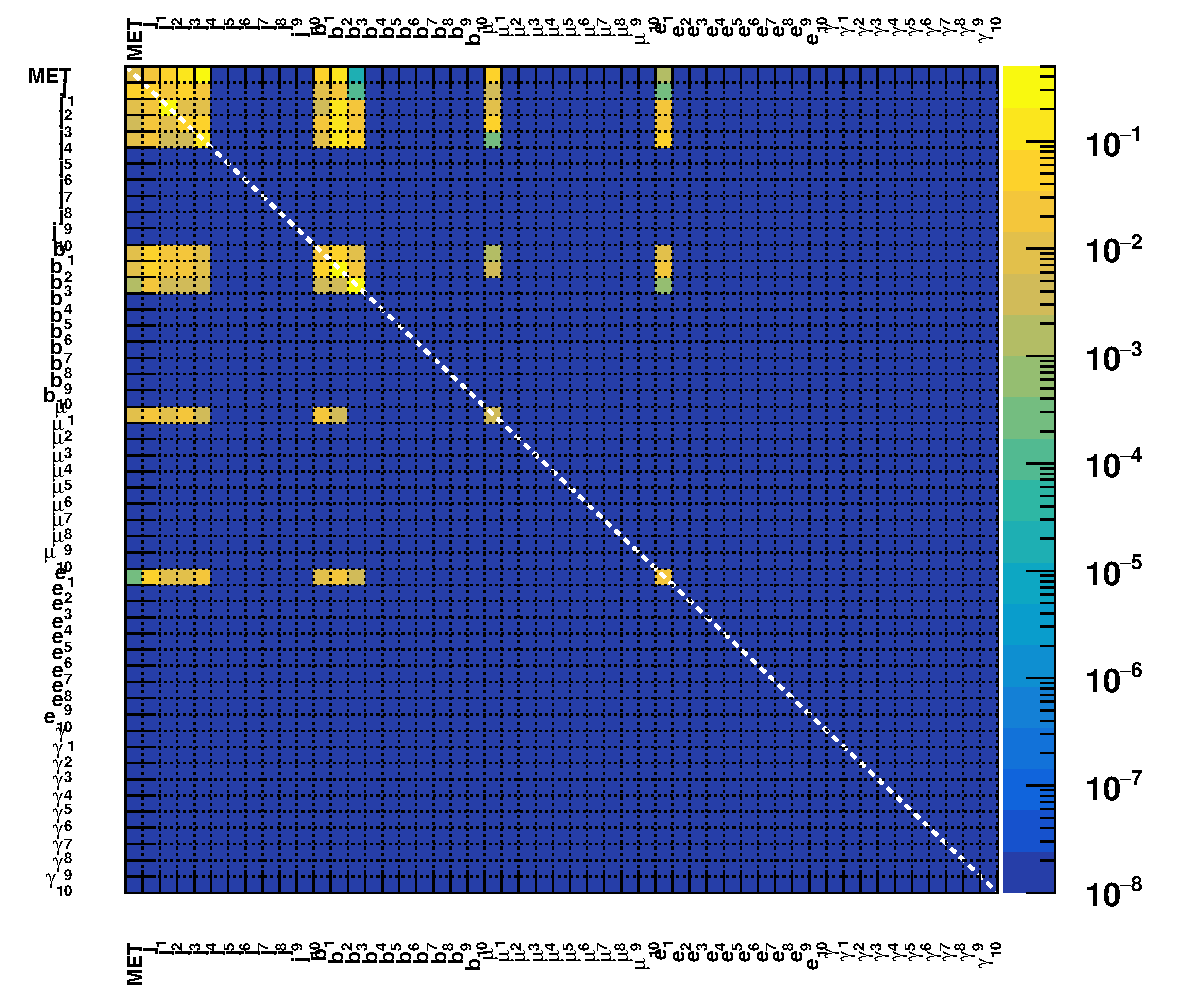
\includegraphics[width=0.9\textwidth]{figs/app/validate_event1_hsplus.pdf}
    \end{center}
    \caption{
    A typical event for the charged Higgs production in association with a top quark, $tbH^{+}$.
    The mass of $H^{+}$ is set to 2 TeV.
    decaying to 2 jets, with the leptonic decay of $W$.
    The event features many jets, $b-$jets, leptons and some  MET.
    }
    \label{fig:rmm_tt3}
\end{figure}

\begin{figure}[H]
    \begin{center}
        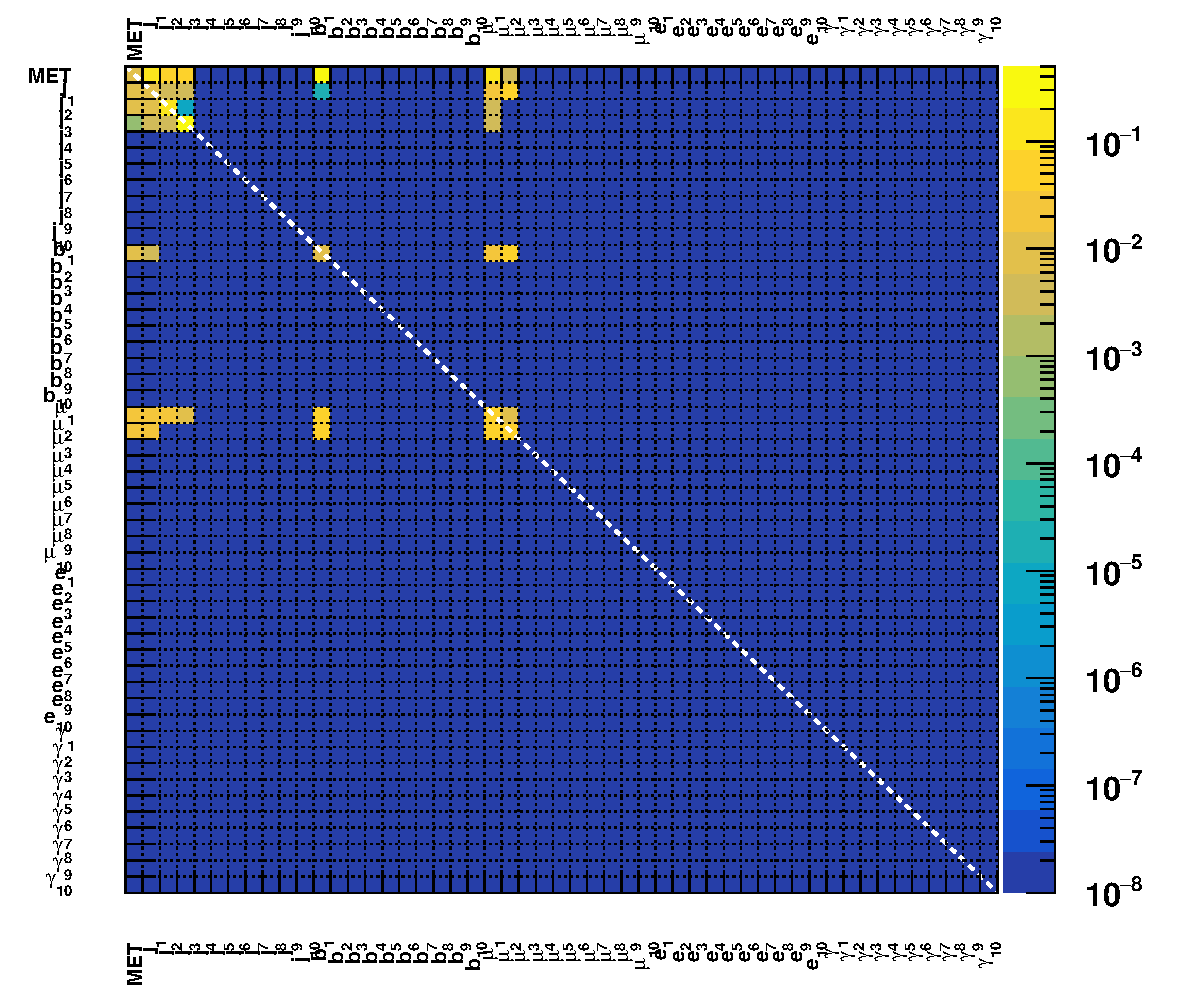
\includegraphics[width=0.9\textwidth]{figs/app/validate_event1_complep.pdf}
    \end{center}
    \caption{
    A typical event for a composite lepton $E$ from a decay of massive $Z'$ with various $Z'$ mass hypotheses.
    The mass of $Z'$ is set to 3 TeV.
    The event features jets, $b-$jets, 2 muons  and some  MET.
    }
\label{fig:rmm_tt4}
\end{figure}

\begin{figure}[H]
    \begin{center}
        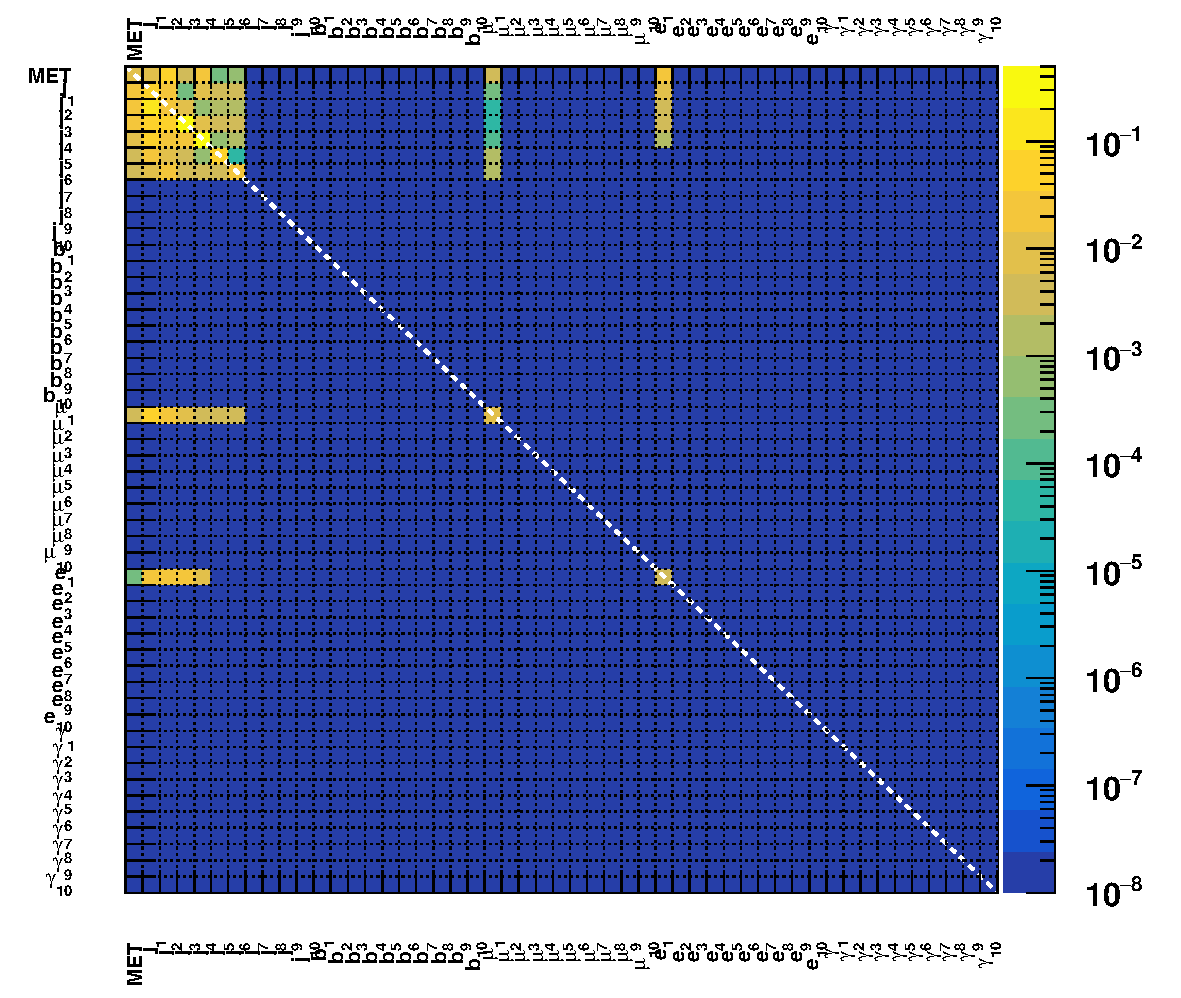
\includegraphics[width=0.9\textwidth]{figs/app/validate_event1_radion.pdf}
    \end{center}
    \caption{
    A typical event for
    a Kaluza--Klein (KK) gauge boson, $W_{kk}$, with a SM $W$ boson and a radion.
    The mass of $W_{kk}$ is set to 4 TeV. 
    The event features many jets, $b-$jets, leptons and some  MET.
    }
\label{fig:rmm_tt5}
\end{figure}
\newpage

\vspace*{0.5in}

\section{Autoencoder Topology Studies}
\label{appendix:ae-topo-studies}
%\addcontentsline{toc}{chapter}{Autoecoder Topology Studies}
\numberwithin{equation}{chapter}
\setcounter{equation}{0}

Ten different topologies were studied for this analysis along with different types of \gls{ae}s such as variational \gls{ae} and the convolutional \gls{ae}. The optimization metrics that were focused on was the 
separation power between \gls{sm} and \gls{bsm} events, along with loss value range. Having a larger range of loss values indicates the every small nuance within the data representation plays a role in data 
separation, which is key for anomaly detection. The separation corresponed with the number of neurons within the dense layers of the encoder and decoder. The nominal architecture may have been increased but was capped 
due to available computational power. 
\par
Hand-made anomalies were created using the $\textrm{W}'$ / $\textrm{Z}'$ \gls{bsm} events with the mass of 4 TeV. Anomaly 1 is when all jets beyond the sub-leading jet were set to he photons and anomaly 2
is when all the jets beyond the sub-leading jet are set to b-jets. High multiplicity of photons and b-jets are considered rare within the \gls{sm} and are expected to be scored as anomalous. Figure~\ref{fig:RMM_SSM_anomaly}
shows each of these three cases. 

\begin{figure}[H]
    \begin{center}
        \subfloat[SSM model] {
            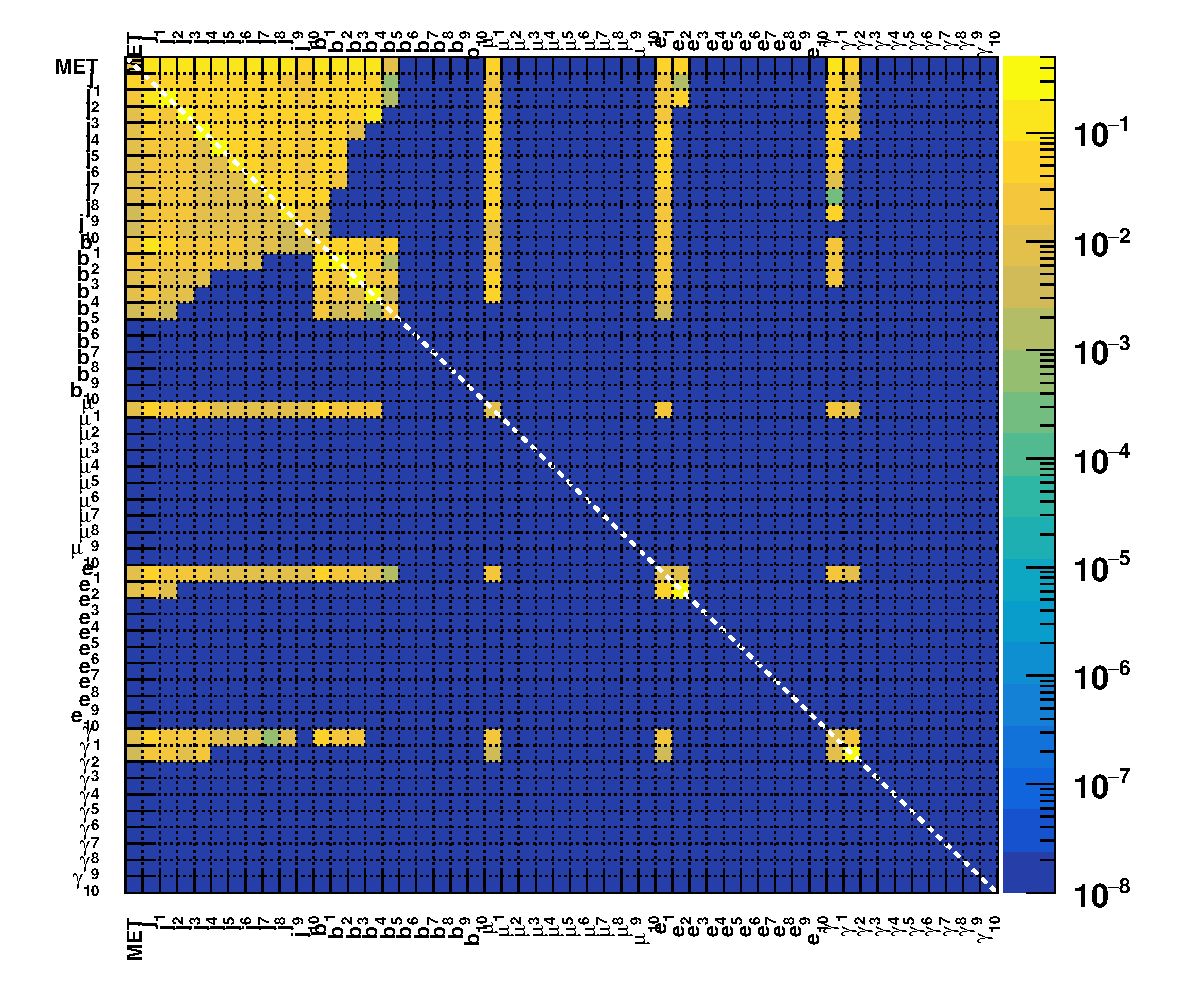
\includegraphics[width=0.33\textwidth]{figs/app/validate_ssm.pdf}
        }
        \subfloat[Anomaly 1] {
            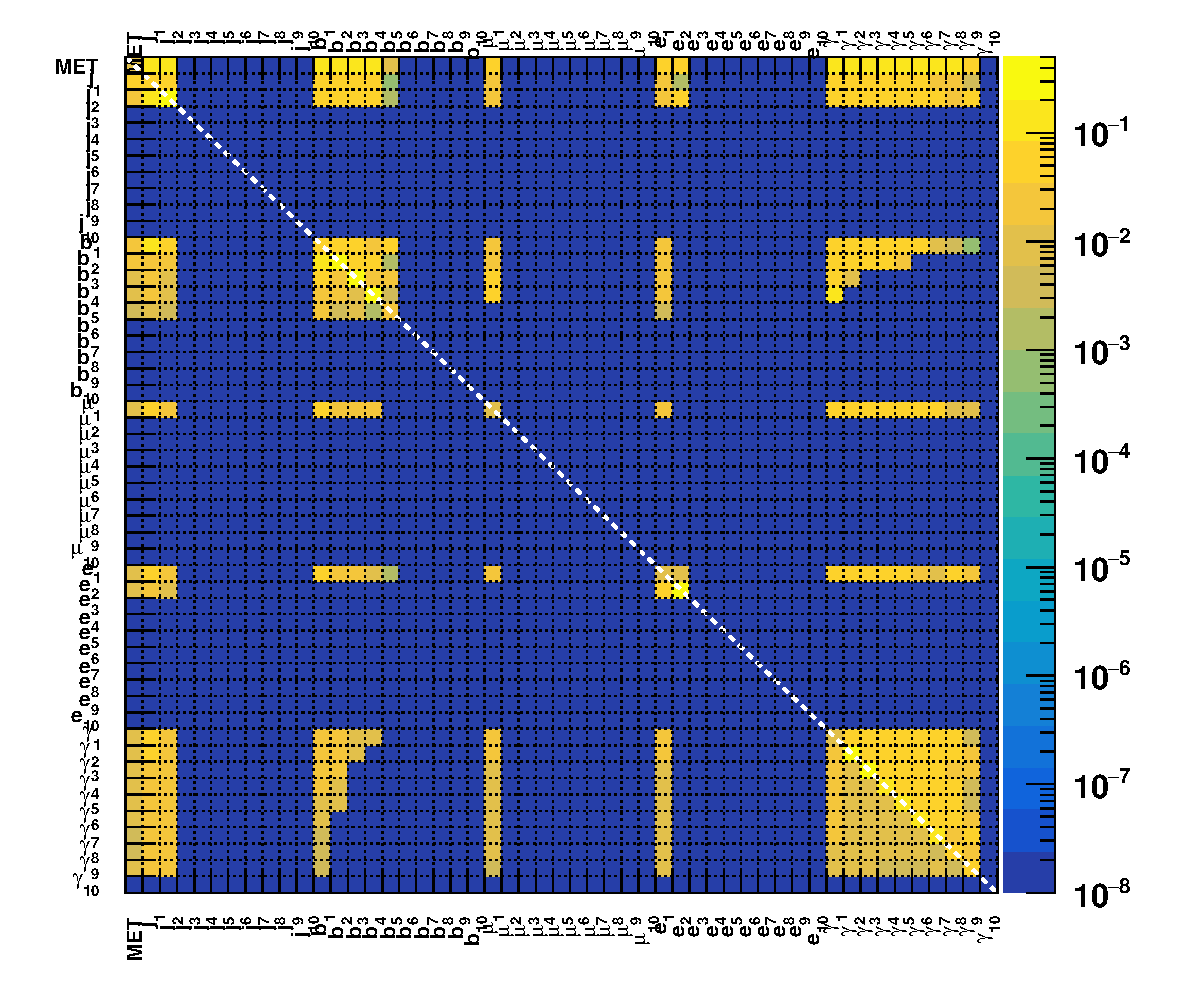
\includegraphics[width=0.33\textwidth]{figs/app/validate_ssm_anomaly1.pdf}
        }
        \subfloat[Anomaly 2] {
            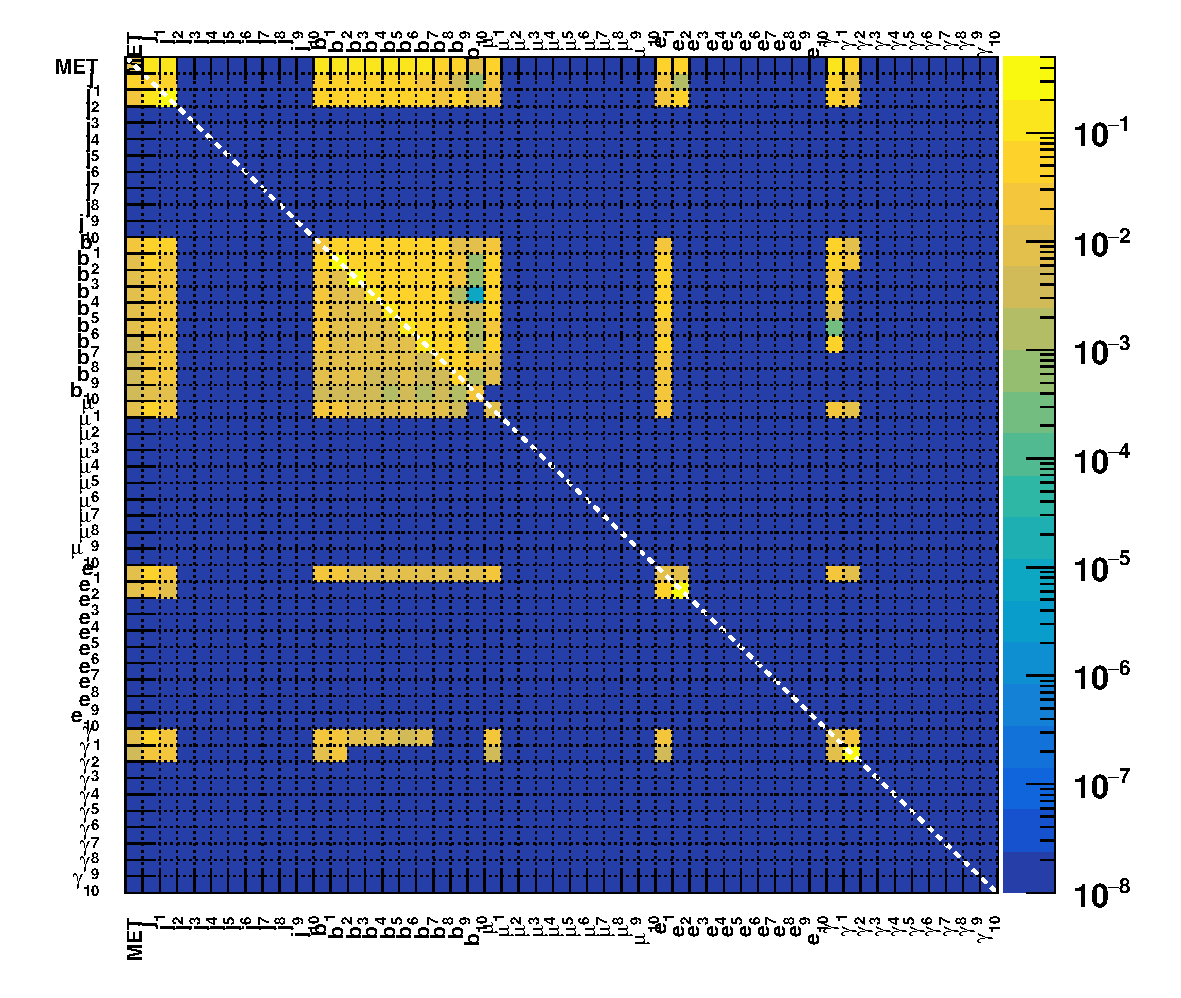
\includegraphics[width=0.33\textwidth]{figs/app/validate_ssm_anomaly2.pdf}
        }
    \end{center}
    \caption{
        An example RMM matrix of a random event from SSM (a), from which jets beyond the sub-leading jet are set to be photons (b) or $b$-jets (c).
    }
    \label{fig:RMM_SSM_anomaly}
\end{figure}

The nominal \gls{ae} architecture as seen in Table~\ref{tab:ae-arch} is ``800-400-200-400-800'' is used to predict the loss values for these samples in Figure~\ref{fig:SSM_losses}. The loss value take for scoring anomalies is the Logarithm of the 
loss value in order to obtain human friendly values while also having a larger distribution. Figure X shows the nominal architecture along with three others (``400-200-100-200-400'', ``200-100-50-100-200'', and ``100-50-25-50-100'') for 
comparison. The bottom two loss plots also show the two types of \gls{ae}s (VAE and CVAE). As seen from these figures, the nominal architecture shows the best separation between \gls{ssm} events (``Before anomaly'')
and the hand-made anomalies as discussed above. 

\begin{figure}[H]
    \begin{center}
        \subfloat[800-* topology] {
            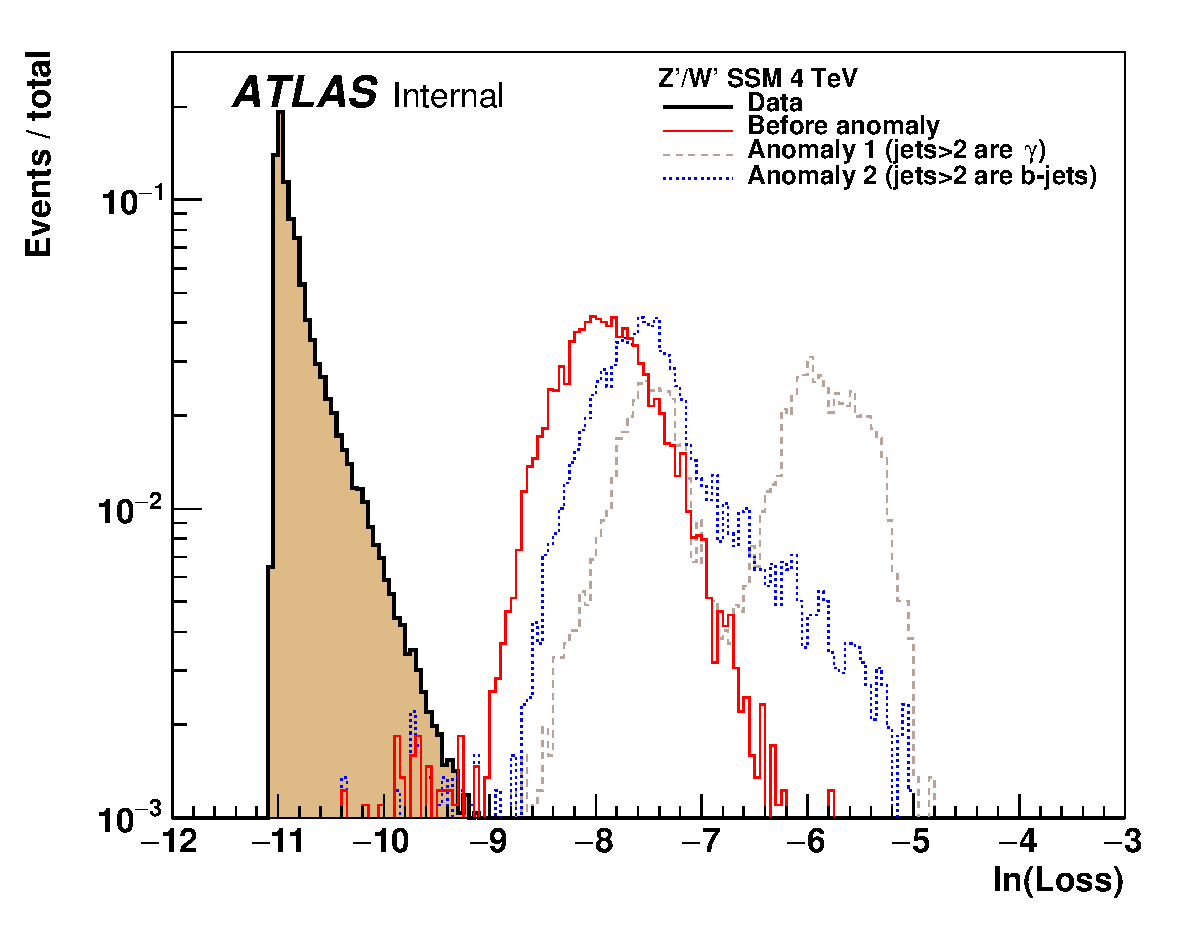
\includegraphics[width=0.45\textwidth]{figs/app/800x400x200x400x800.pdf}
        }
        \subfloat[200-* topology] {
            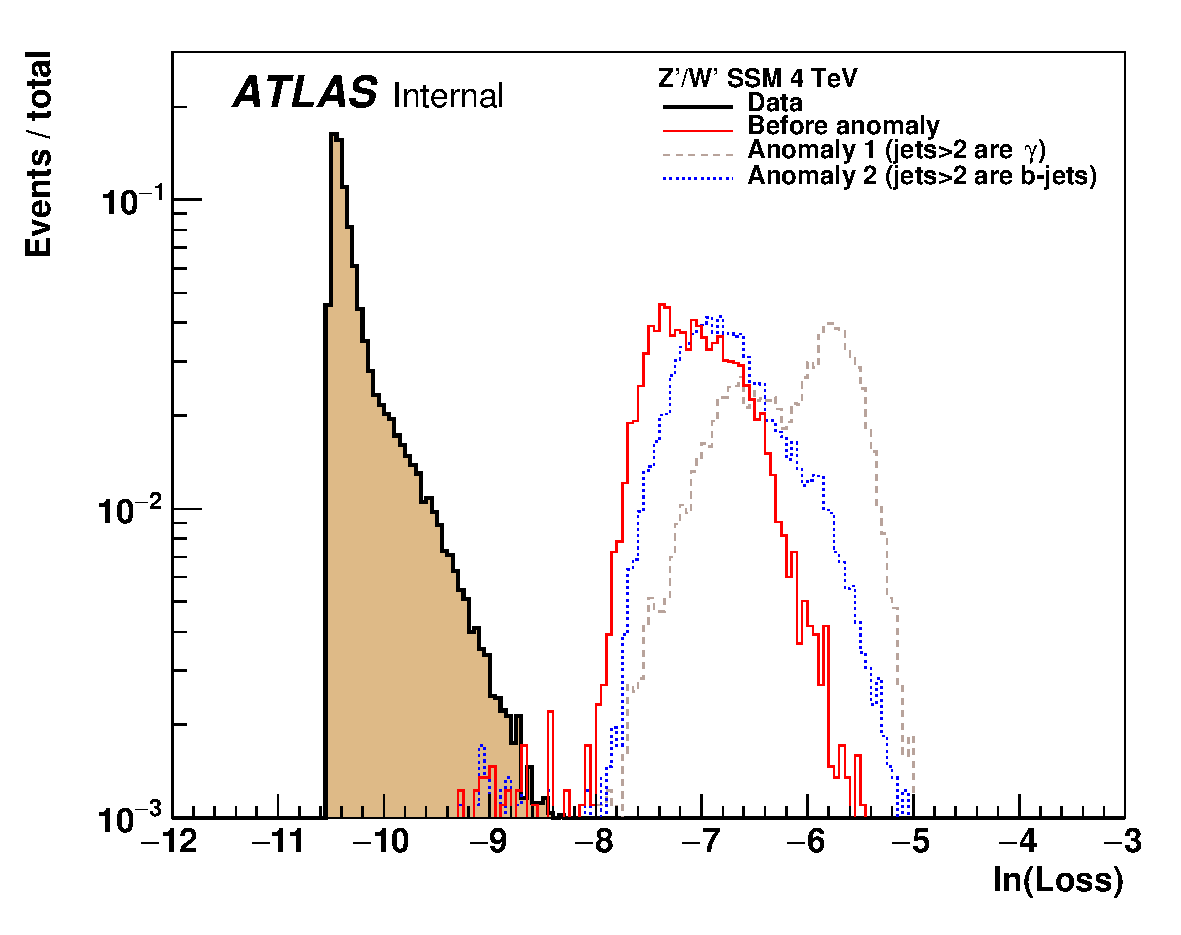
\includegraphics[width=0.45\textwidth]{figs/app/200x100x50x100x200.pdf}
        } \\
        \subfloat[100-* topology] {
            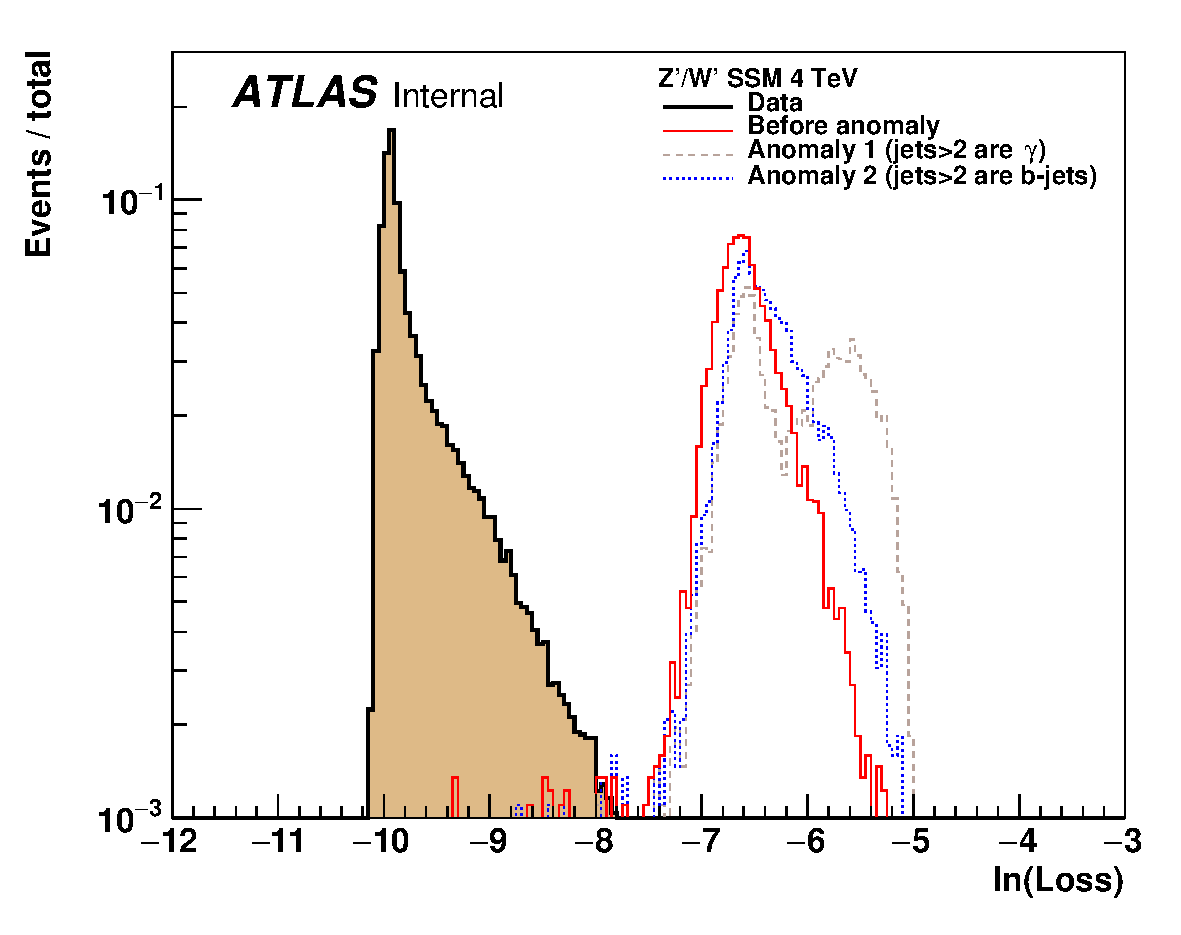
\includegraphics[width=0.45\textwidth]{figs/app/100x50x25x50x100.pdf}
        }
        \subfloat[20-* topology] {
            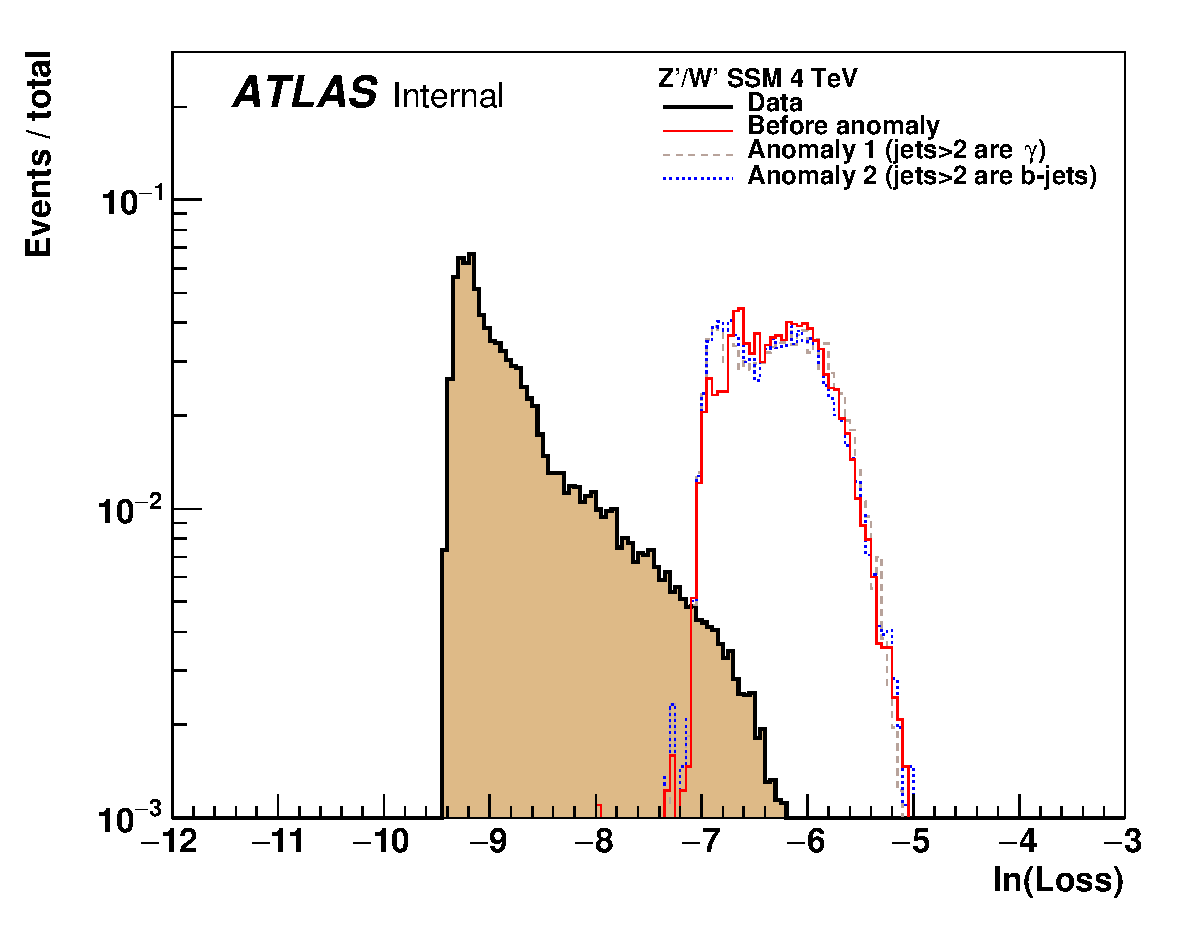
\includegraphics[width=0.45\textwidth]{figs/app/20x10x5x10x20.pdf}
        } \\
        \subfloat[Variational AE topology] {
            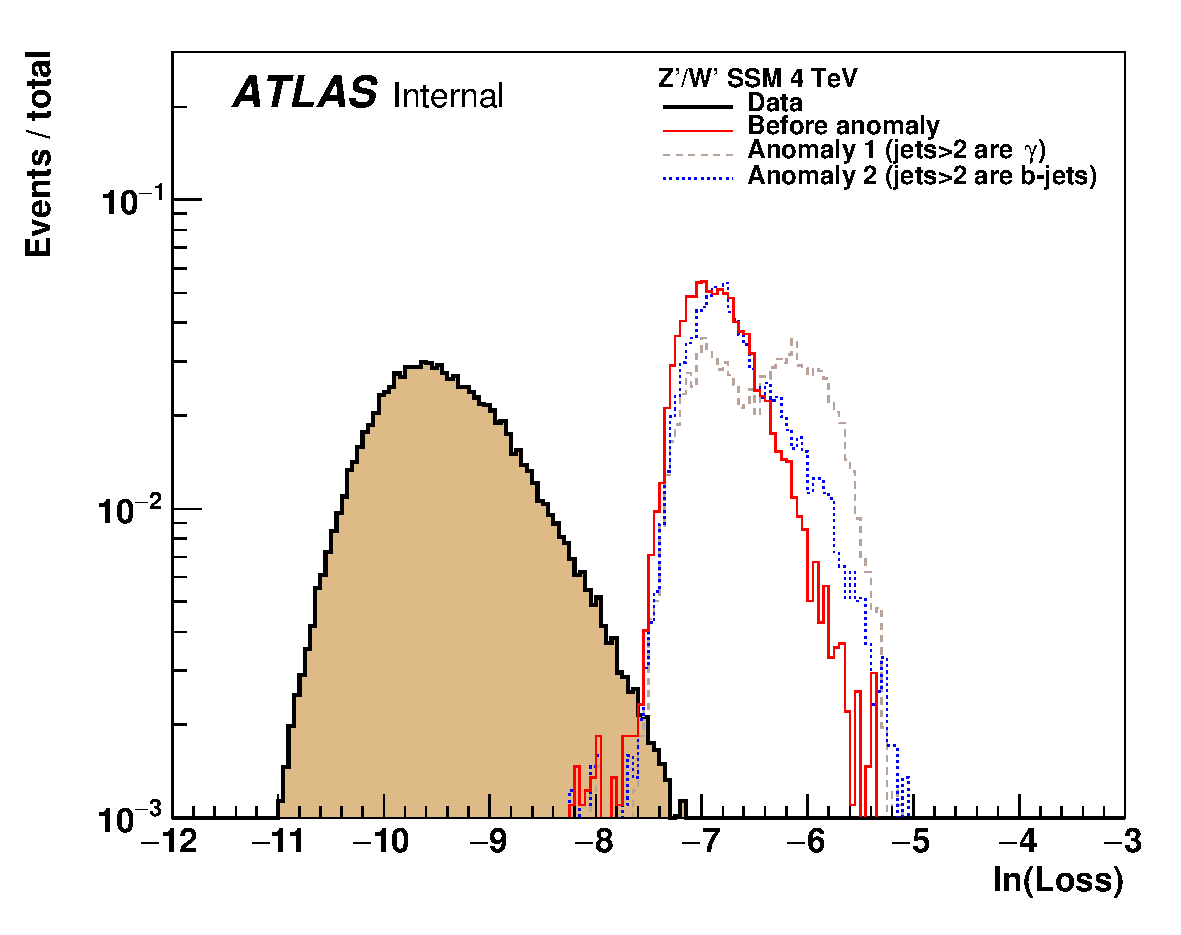
\includegraphics[width=0.45\textwidth]{figs/app/mass_wzsim_data_anomaly_loss_vae.pdf}
        }
        \subfloat[Convolutional VAE topology] {
            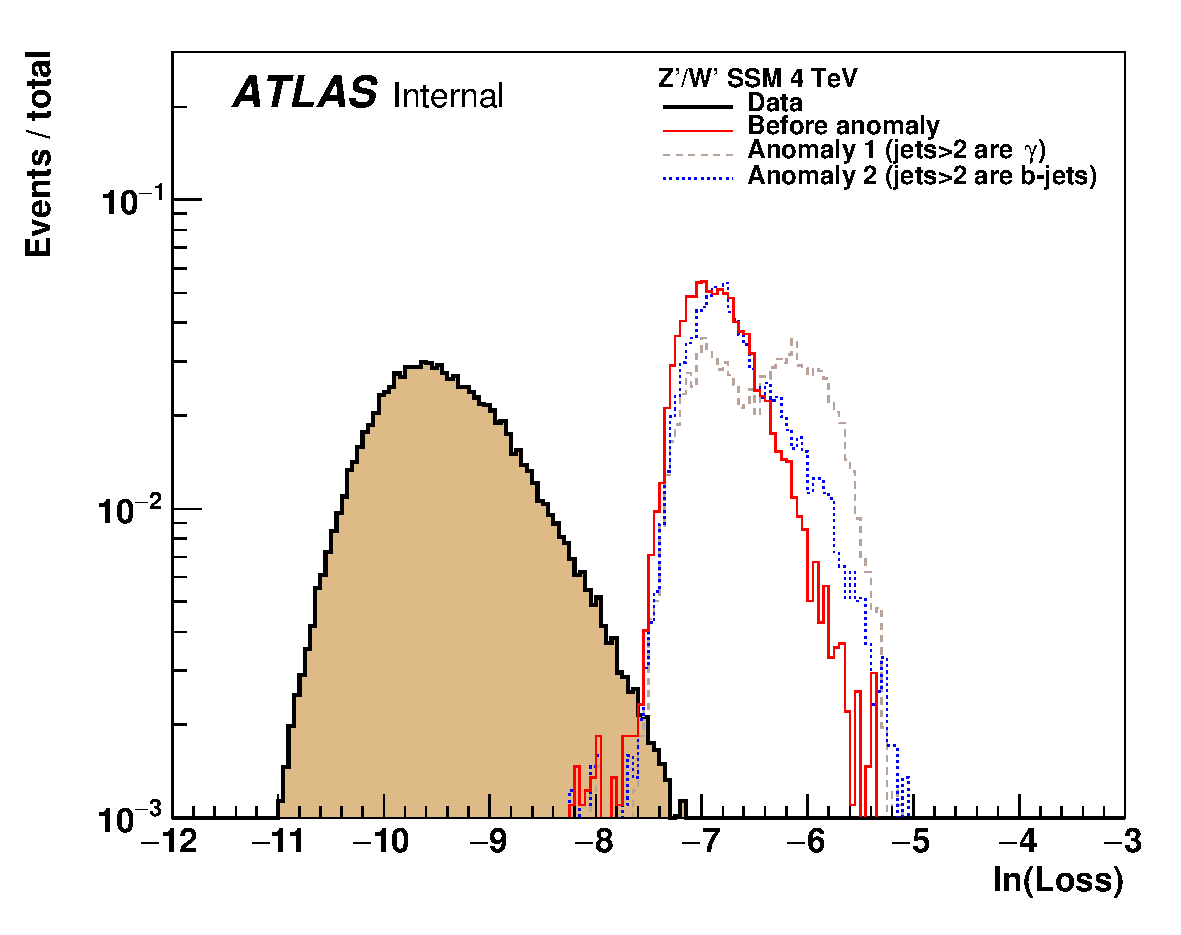
\includegraphics[width=0.45\textwidth]{figs/app/mass_wzsim_data_anomaly_loss_cvae.pdf}
            \label{fig:SSM_losses_d}
        }
    \end{center}
        \caption{
            The loss distributions for the original SSM with 4 TeV Z' and for anomaly 1 and 2.
        }
\label{fig:SSM_losses}
\end{figure}

\newpage

\vspace*{0.5in}

\section{Alternative AE Models for Systematics}
\label{appendix:ae-systematics}
%\addcontentsline{toc}{chapter}{Alternative AE Models for Systematics}
\numberwithin{equation}{chapter}
\setcounter{equation}{0}

As discussed in Section~\ref{sec:ae-training}, three models were training using the optimized architecture after 50 trainings were conducted. The nominal refers to the mean 
loss model, the ``up'' and ``down'' models correspond to the slightly higher anad lower loss values. The performances of these three models are evaluated on \gls{bsm} signals in 
Figure~\ref{fig:roc_rms}. The outlier regions that are used will have low signal efficiency (low x on these plots). The performances are consistent.

\begin{figure}[H]
    \begin{center}
    \subfloat[Composite leptons low mass] {
        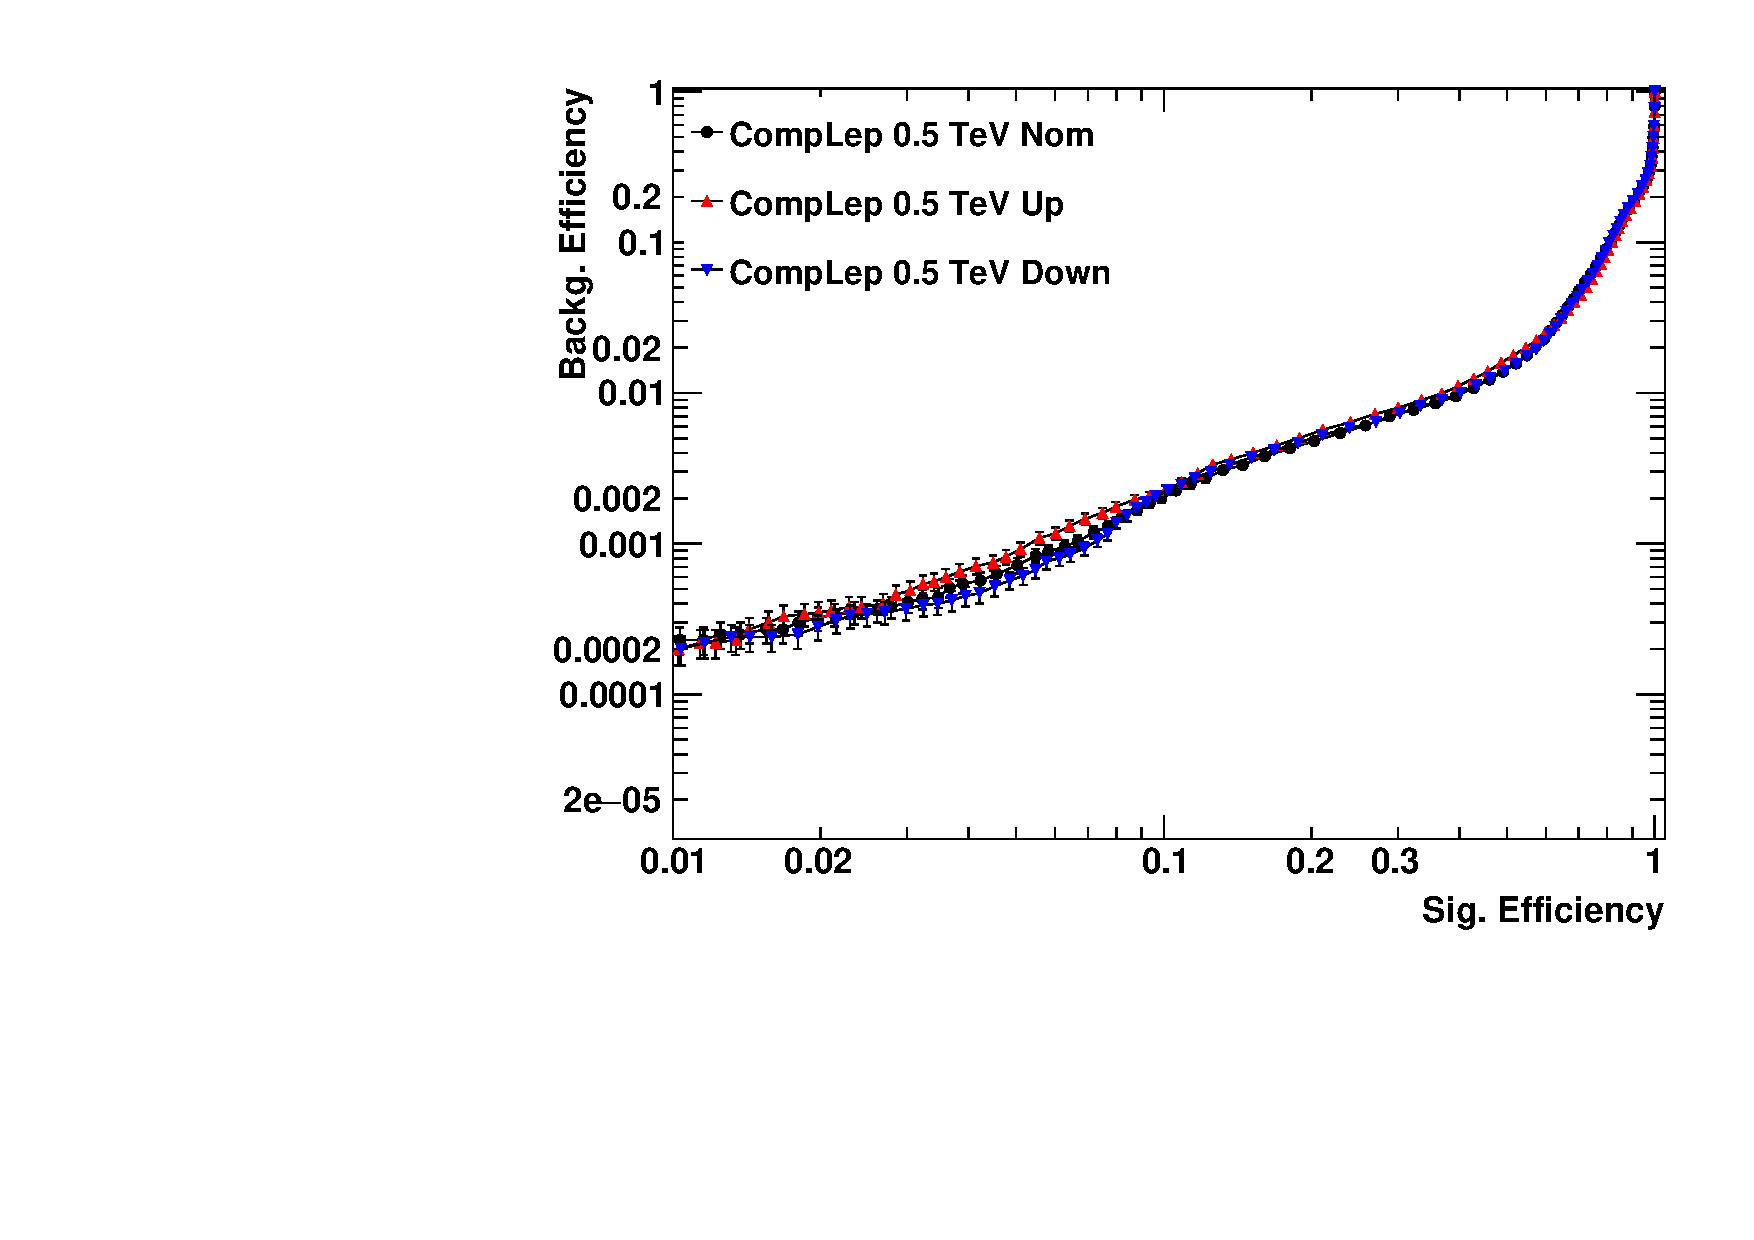
\includegraphics[width=0.45\textwidth]{figs/ch6/roc/ROC_CompLep_low.pdf}
    }
    \subfloat[Composite leptons high mass] {
        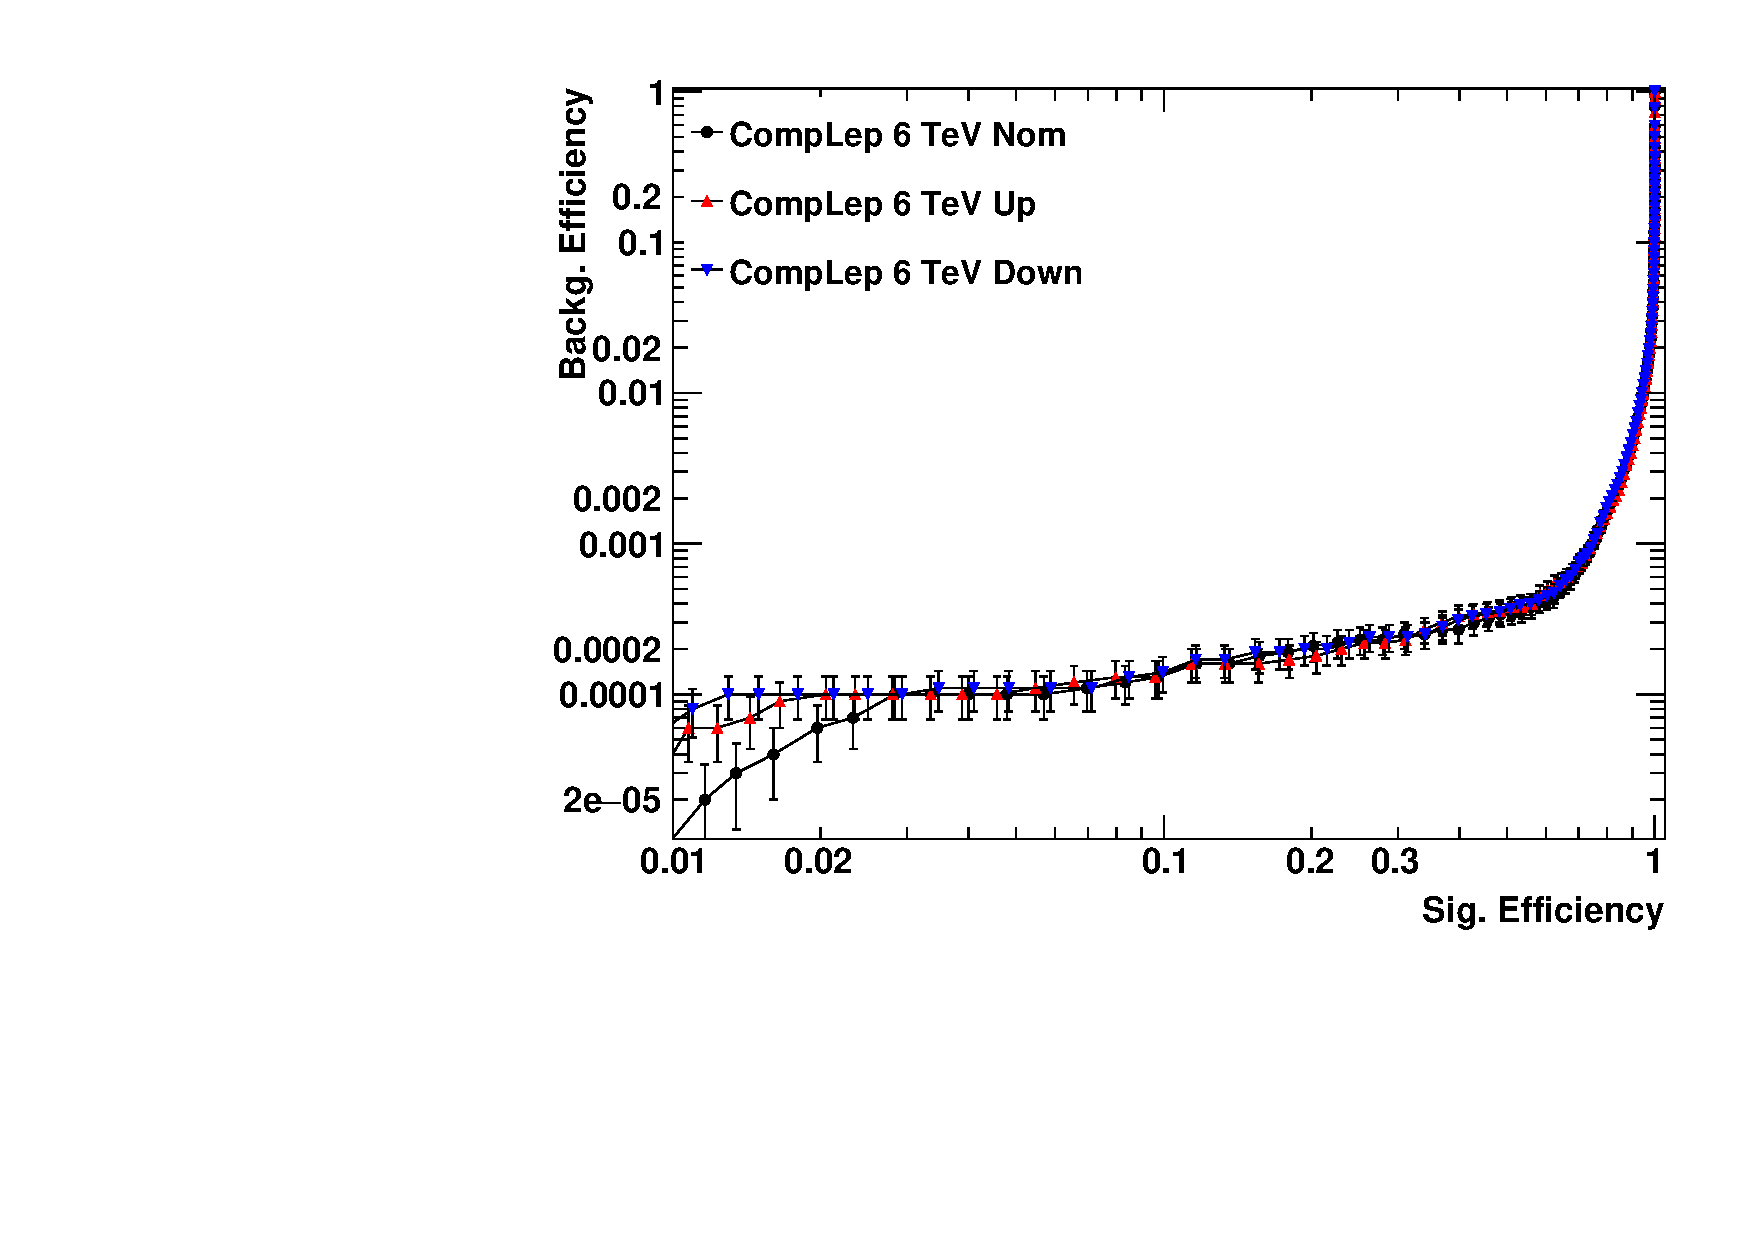
\includegraphics[width=0.45\textwidth]{figs/ch6/roc/ROC_CompLep_high.pdf}
    } \\
    \subfloat[Radion low mass] {
        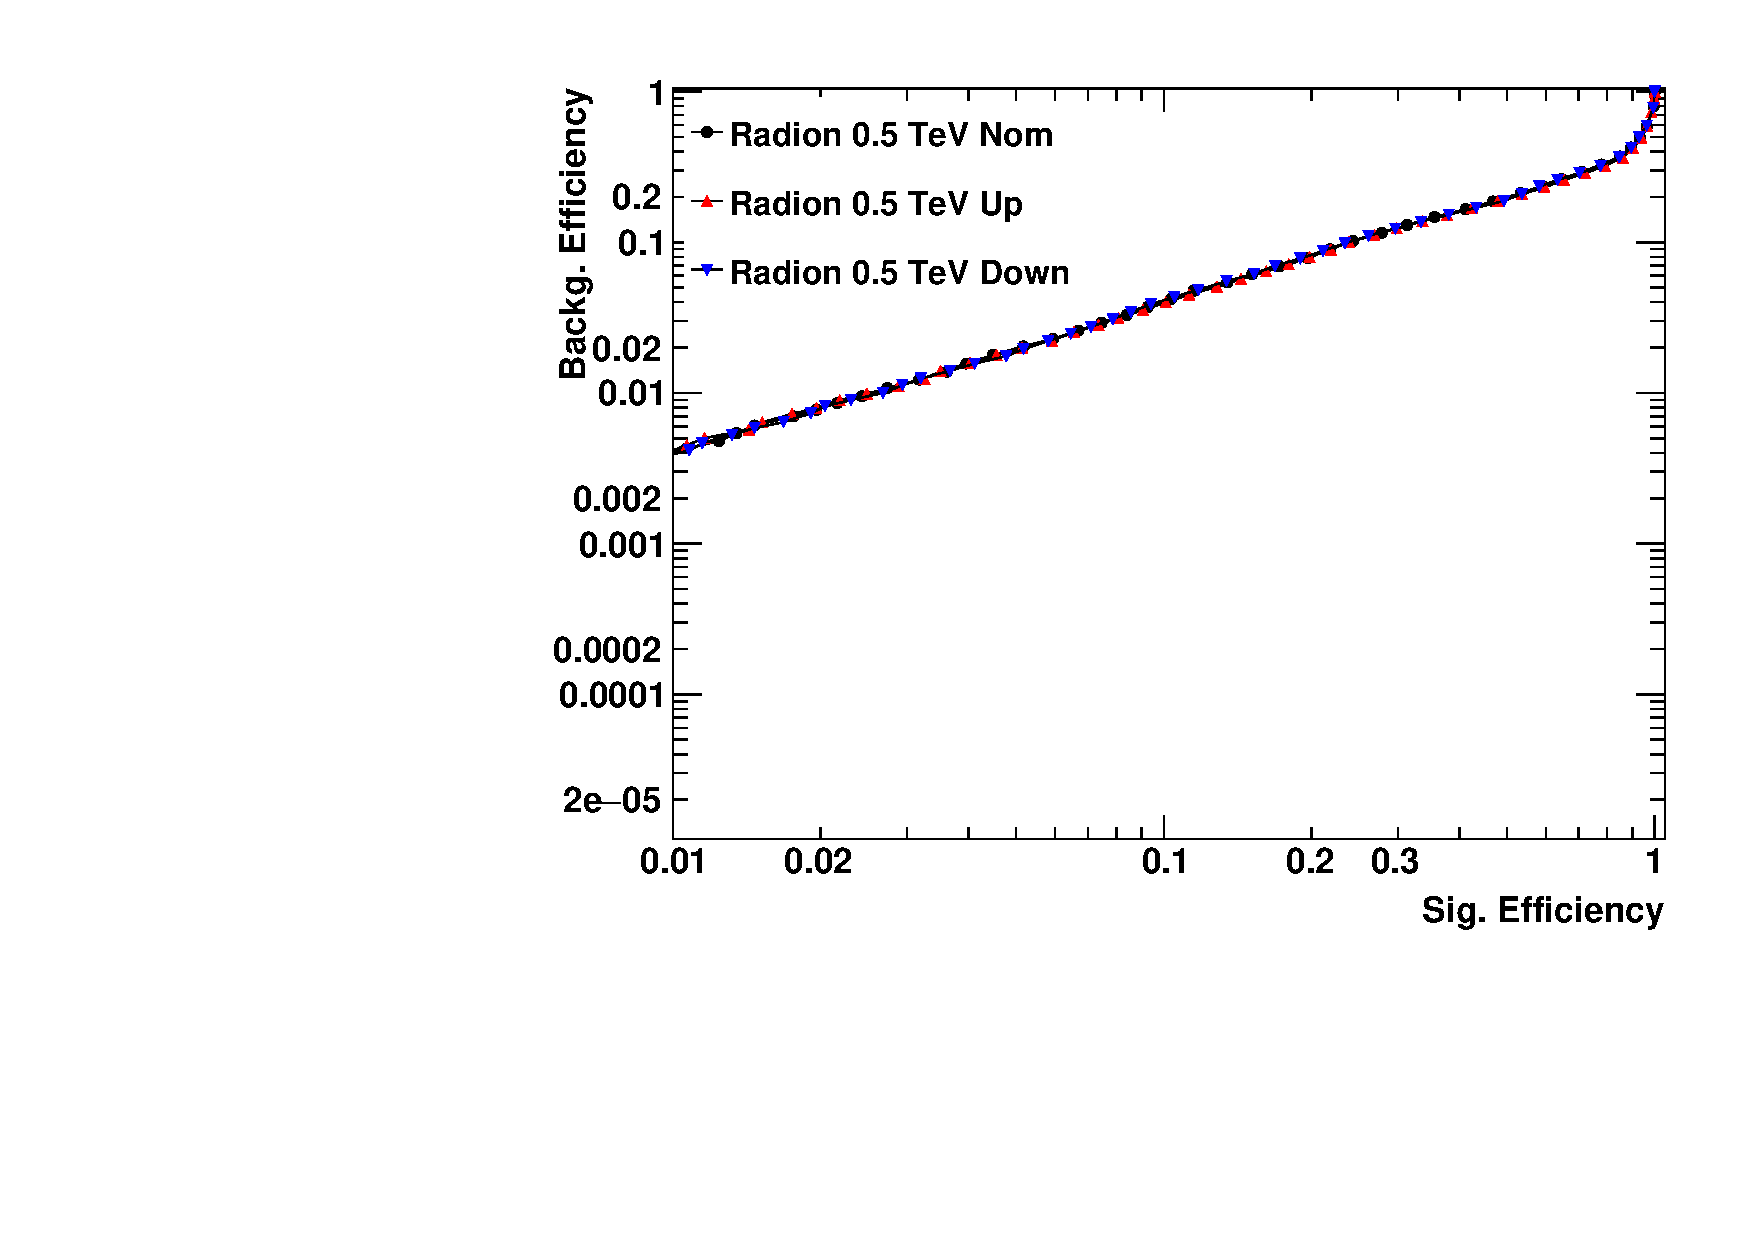
\includegraphics[width=0.45\textwidth]{figs/ch6/roc/ROC_Radion_low.pdf}
    }
    \subfloat[Radion high mass] {
        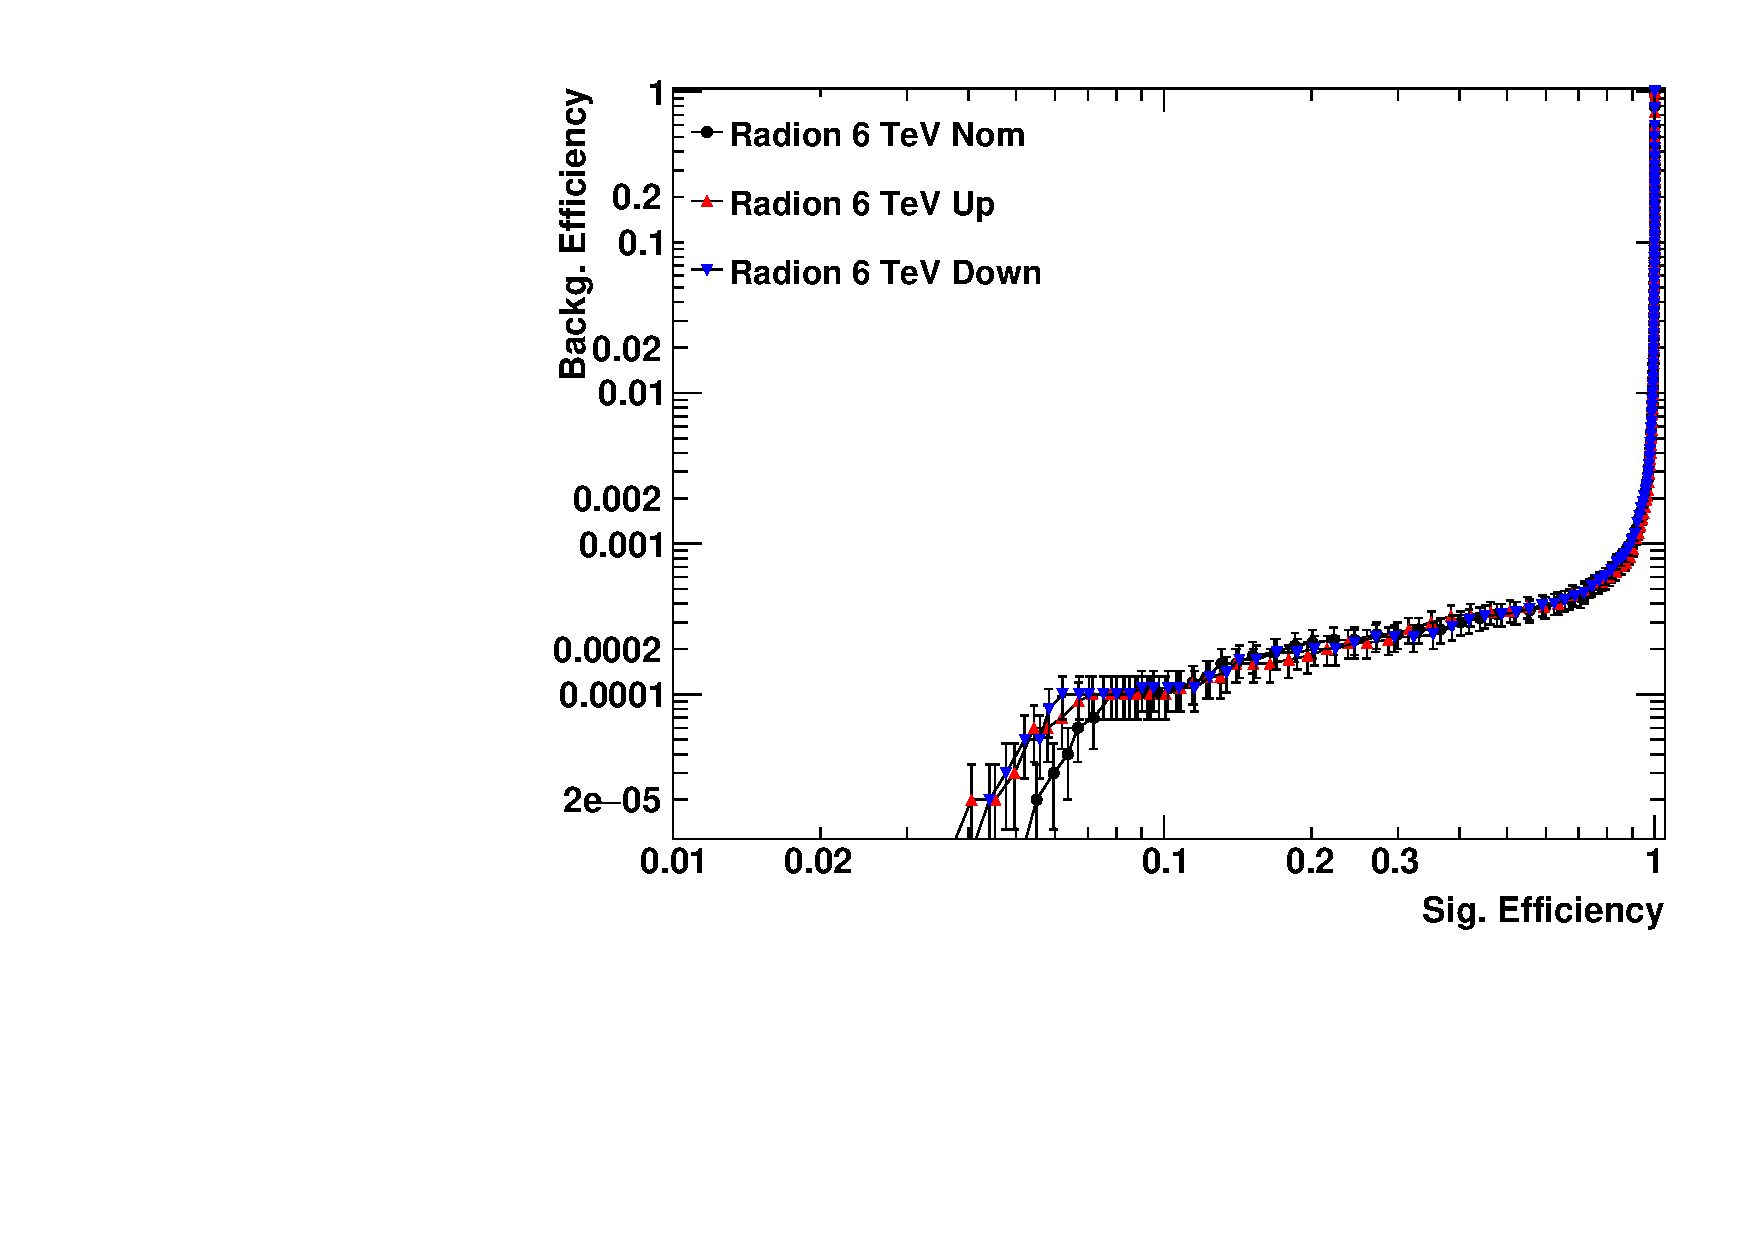
\includegraphics[width=0.45\textwidth]{figs/ch6/roc/ROC_Radion_high.pdf}
    } \\
    \subfloat[W'/Z' low mass] {
        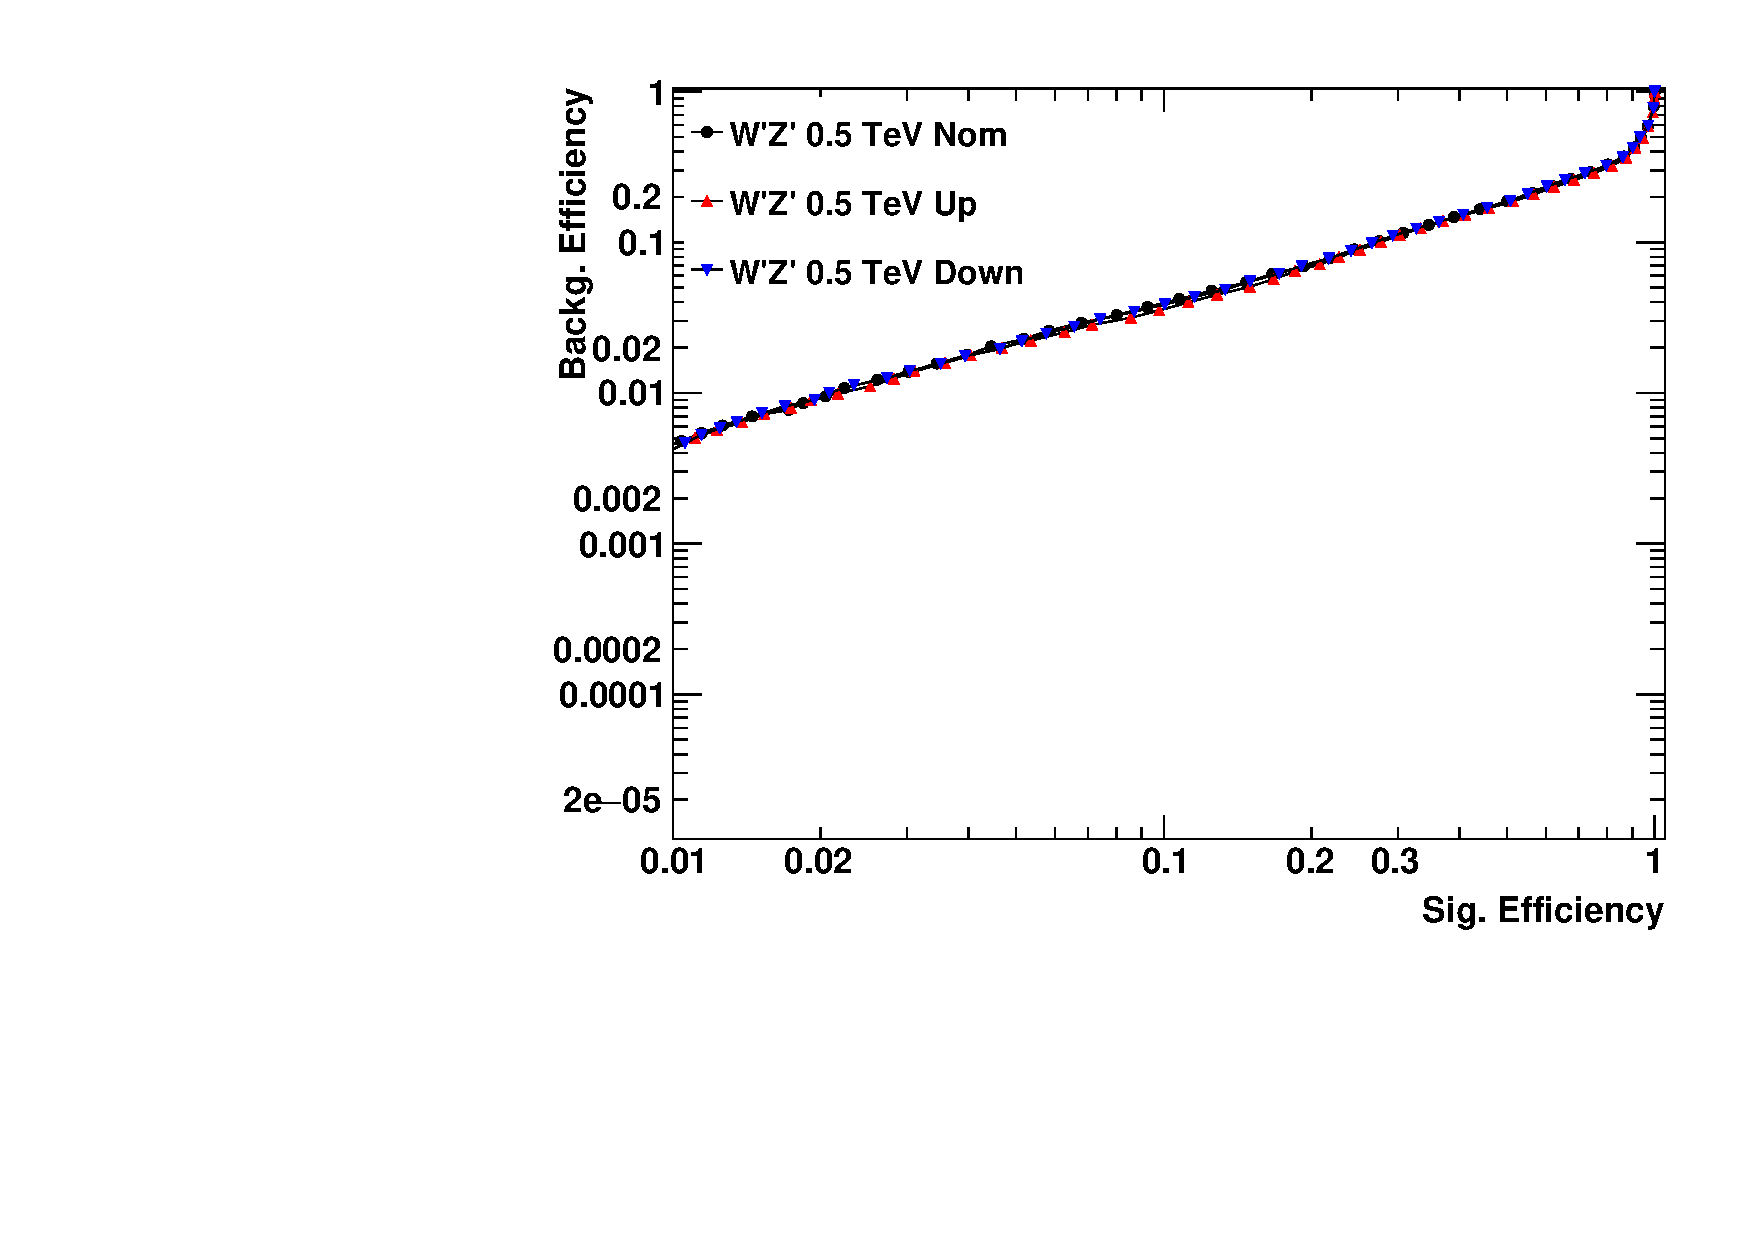
\includegraphics[width=0.45\textwidth]{figs/ch6/roc/ROC_WZprime_low.pdf}
    }
    \subfloat[W'/Z' high mass] {
        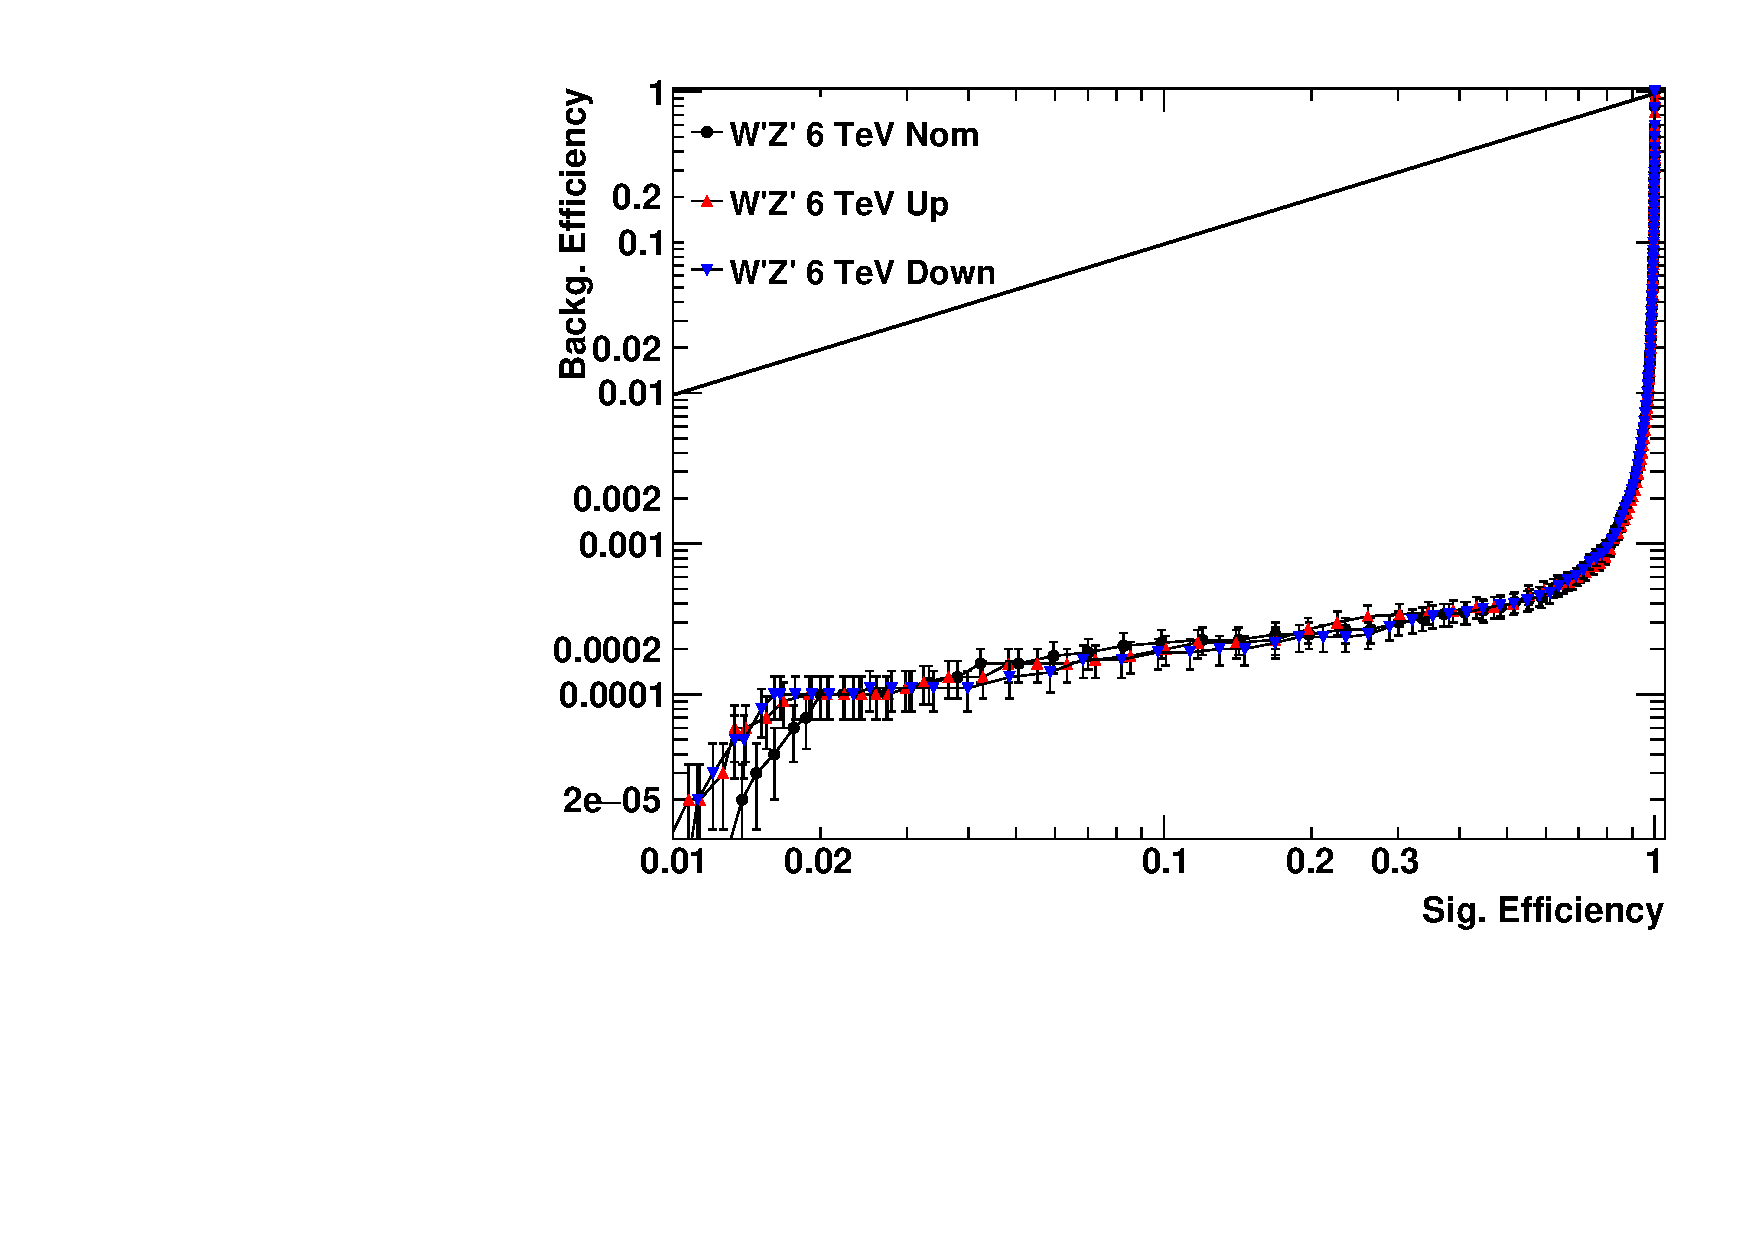
\includegraphics[width=0.45\textwidth]{figs/ch6/roc/ROC_WZprime_high.pdf}
    } \\
    \end{center}
    \caption{
        Background efficiency vs signal efficiency of various BSM models under different mass hypotheses, using the nominal and alternative AE models.
        Note there are some artificial lines due to plotting issues.
    }
\label{fig:roc_rms}
\end{figure}

\newpage

\vspace*{0.5in}

\section{S/B Improvement Example}
\label{appendix:sb-improvements}
%\addcontentsline{toc}{chapter}{Autoencoder S/B Improvement Example}
\numberwithin{equation}{chapter}
\setcounter{equation}{0}

There are many factors that determine the how well the S/B increases after an anomaly score cut, such as topology of the final states, the mass of heavy particles, the type of di-object invariant mass, the chosen \gls{ar}
working point, etc. It is expected that the more ``exotic'' the \gls{bsm} model is, the more it deviates from the \gls{sm} background. Therefore, it's expected that the heavier the \gls{bsm} resonance is, the higher 
the anomaly score will be given, resulting in a large S/B calculation. 
\par
The following is an example using the radion \gls{bsm} model due to its rather complex decay topology in two-body (even three-body) mass. The radion particle decays from a Kaluza-Klein boson Wkk into a 
radion denoted by $\varphi$ as seen in:

$$
Wkk \to W + \varphi \to l\nu + gg
$$

where the events should have \gls{met} as there is a neutrino due to the W decay. The invariant mass that's focused on within this example is the jet+electron ($\textrm{m}_{\textrm{je}}$) since the final state is 
a semi-leptonic decay. The mass resonance used for the Wkk boson is 2 TeV decaying to a $\varphi$ = 500 GeV. Figure X shows the signal event yields before and after the 10 pb \gls{ar} cut while also showing 
the \gls{mc} background yields that include the loose electron control region (\gls{le-cr}) which is a data-driven multi-jet estimation (discussed in Section X). Table~\ref{tab:signal-reduction-radion} shows the numerical values for these yields
after the 10 pb \gls{ar}. The $\textrm{S}/\textrm{B}$ is increased by \~500\%. The discovery sensitivity~\cite{disc-sens} is calculated using the Eq.~\ref{eq:app:1.1}.

\begin{equation}\label{eq:app:1.1}
    Z_A = \sqrt{2 \left(  (s+b)\ln \left( 1+\frac{s}{b} \right) -s \right)}
\end{equation}

is improved by $\textrm{Z}_{\textrm{A}}$= $\sim$80\%. After the 1 pb cut, the $\textrm{S}/\textrm{B}$ is incrased by $\sim$1100\% and $\textrm{Z}_{\textrm{A}}$= $\sim$12\%. 

\begin{figure}[H]
    \centering
    \begin{subfigure}[h]{0.32\linewidth}
    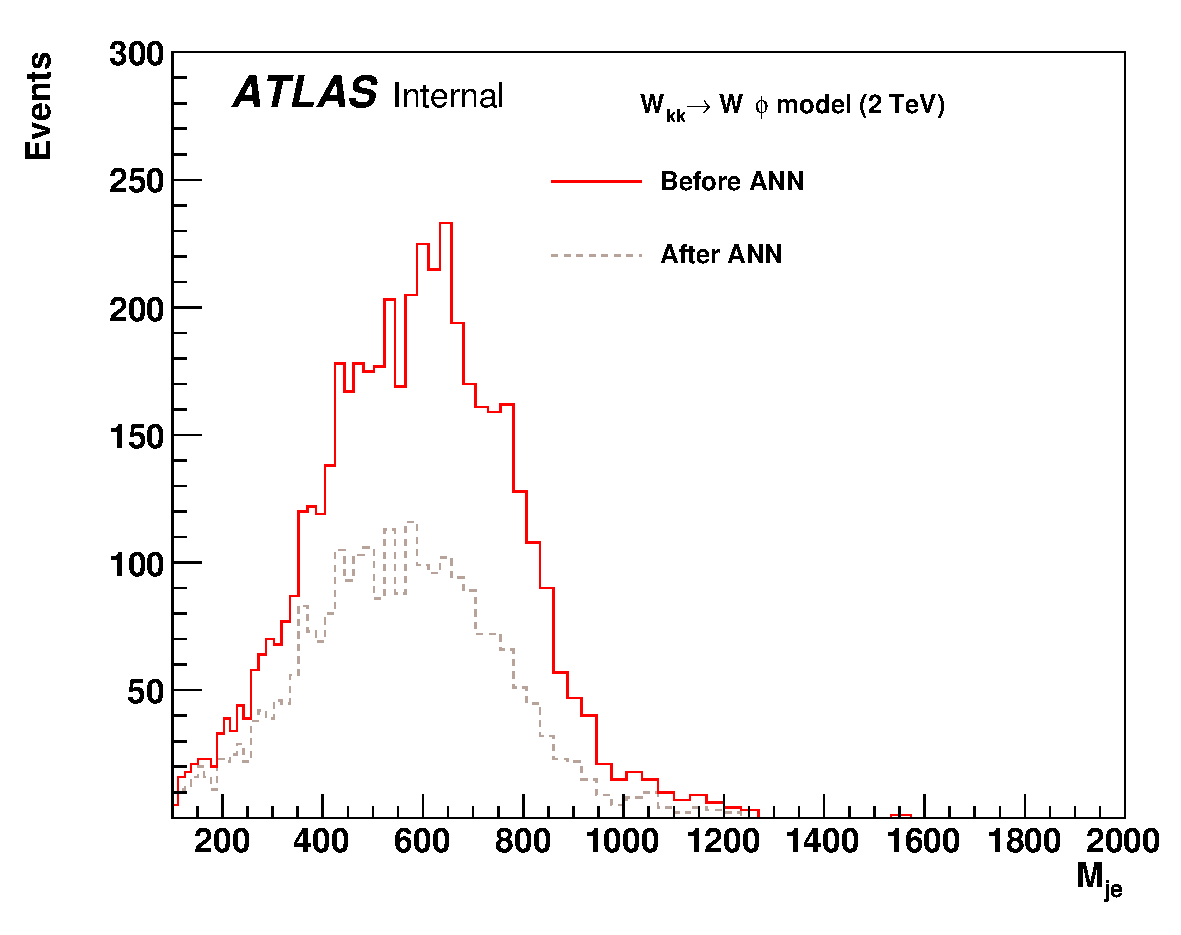
\includegraphics[scale=0.3]{figs/ch6/ar/mass_radion.pdf}%
    \caption{Radion before and after AR cut}
    \end{subfigure}
    \hfill
    \begin{subfigure}[h]{0.28\linewidth}
    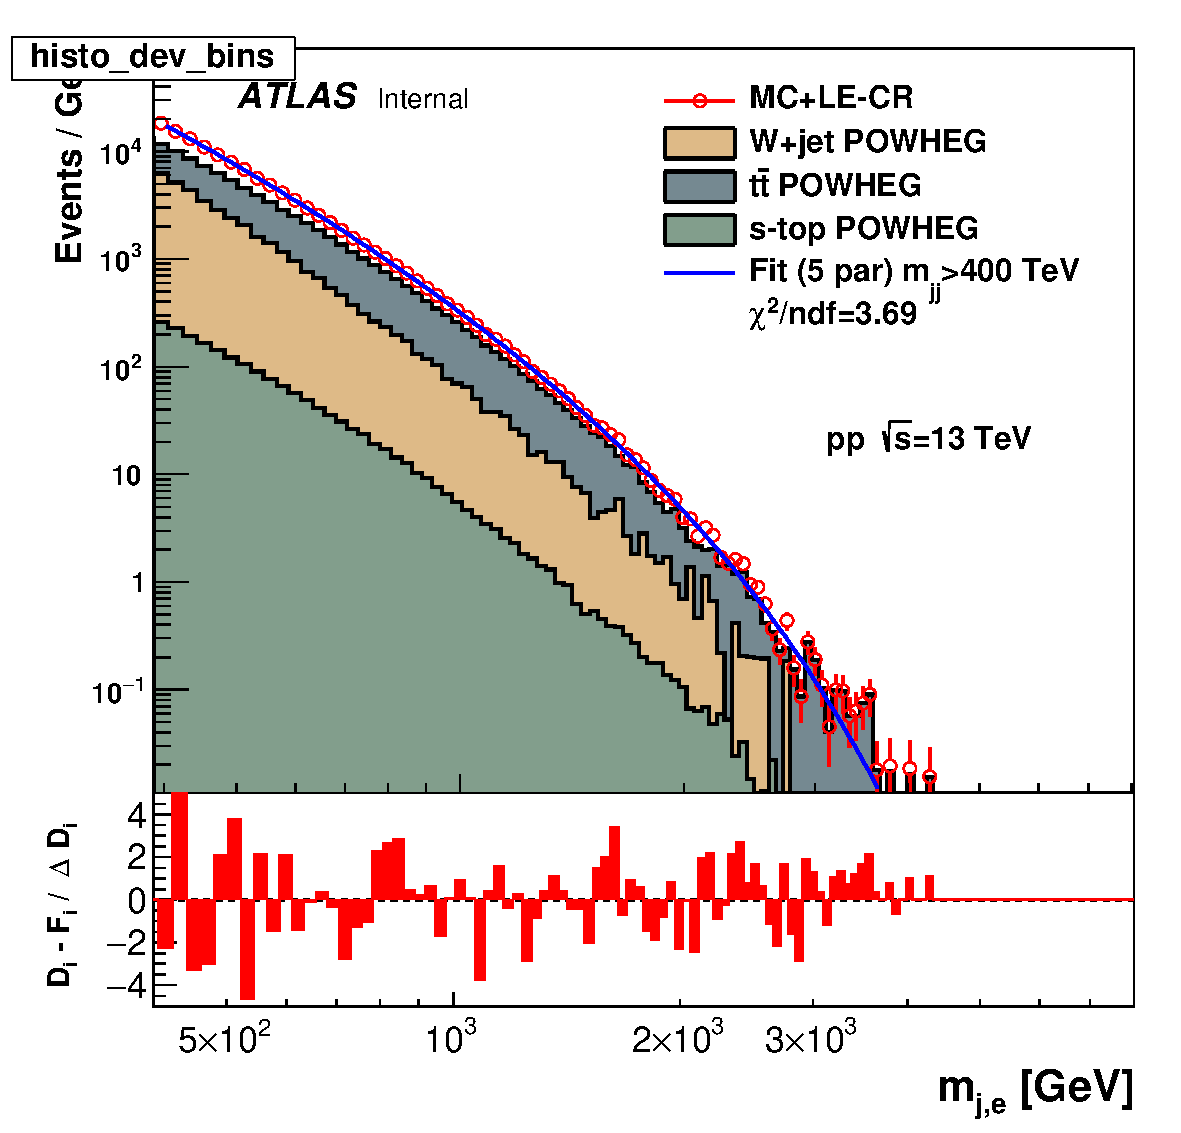
\includegraphics[scale=0.25]{figs/ch6/ar/mass_je_mcCR_before_scale.pdf}%
    \caption{Before AR cut}
    \end{subfigure}
    \hfill
    \begin{subfigure}[h]{0.28\linewidth}
    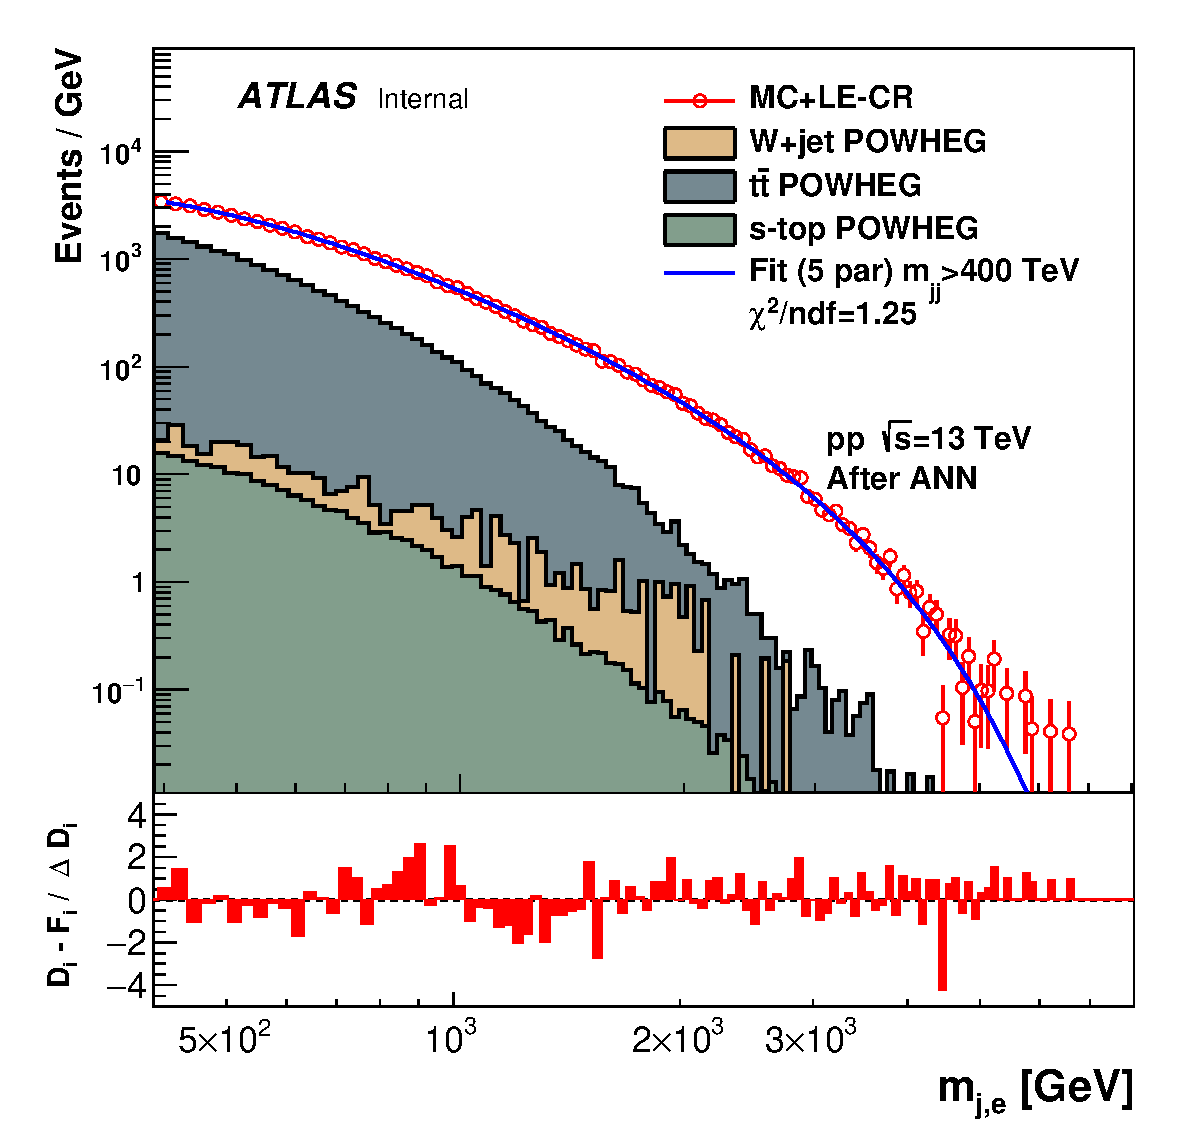
\includegraphics[scale=0.25]{figs/ch6/ar/mass_je_mcCR_after_scale.pdf}%
    \caption{After AR cut}
    \end{subfigure}
    \hfill
    \caption{(a) 500 GeV radion model signal yields before and after the 10 pb AR cut is applied. (b)(c) Comparison background events for the jet+electron invarint mass before and after the 10 pb AR cut. }
\label{fig:sb-yields}
\end{figure}

\begin{table}[!htbp]
    \begin{footnotesize}
    \begin{center}
         \begin{tabular}{lr|rr|rr|rr}
             \hline
                  & {Before cut} &  {10 pb} & {10 pb / Before} &  {1 pb} & {1 pb / Before} &  {0.1 pb} & {0.1 pb / Before}\\
             \hline
             Radion 2 TeV     & 3356     & 1799    & 0.53           & 338        & 0.101       & 65        & 0.0193 \\
             Bkg              & 8999316  & 790230  & 0.087          & 72206      & 0.0080      & 7280      & 0.00081 \\
             $S/B$            & 0.00037  & 0.0022  & 6.10           & 0.0047     & 12.5         & 0.0089    & 24.1 \\
             $Z_A$            & 1.11     & 2.02    & {\bf 1.80}     & 1.25       & {\bf 1.12}       & 0.76      & {\bf 0.68} \\
             \hline
         \end{tabular}
    \end{center}
    \end{footnotesize}
    \caption{Sensitivity gain of the radion model with Wkk set to 2 TeV before and after applying the 10 pb and 1 pb AR cut. Event yields counted in the 400-800 GeV range for the invariant mass $\textrm{m}_{\textrm{je}}$.}
\label{tab:signal-reduction-radion}
 \end{table}

 \newpage

 \vspace*{0.5in}

\section{Statistical Fit Function Studies for 1pb AR}
\label{appendix:1pb-fit-studies}
%\addcontentsline{toc}{chapter}{Statistical Fit Function Studies for 1pb AR}
\numberwithin{equation}{chapter}
\setcounter{equation}{0}

Similar to Section~\ref{sec:bkg-fit-studies}, this appendix shows the studies conducted for the 1 pb \gls{ar}. Since the 5p function showed to be the reasonable out of the three 
tested functions int the 10 pb \gls{ar} region, only the 4p and 5p fit functions are studied for the 1 pb and 0.1 pb \gls{ar}. These plots show the functions in the 
\gls{mc}+\gls{le-cr}. This region has noticable less statistics than the 10 pb region, therefore it's prone to larger statistical fluctuations within the fit functions, 
especially when requiring a b-jet or photon. Due to the minimal amount of statistics, a reasonable fit function that could be used for all nine invariant masses was unable 
to be found. A summary for the 1 pb statistical tests can be found in Table X. The following figures show the fits of the p4 and p5 functions along with their pulls for 
all nine invariant masses. The fit studies for the 0.1 pb region can be found in Appendix X. 

\begin{multicols}{3}
    \begin{itemize}
    \item Figure~\ref{fig:mjj-fit-pulls-1pb} 1pb \mjj
    \item Figure~\ref{fig:mjb-fit-pulls-1pb} 1pb \mjb
    \item Figure~\ref{fig:mbb-fit-pulls-1pb} 1pb \mbb
    \item Figure~\ref{fig:mje-fit-pulls-1pb} 1pb \mje
    \item Figure~\ref{fig:mjm-fit-pulls-1pb} 1pb \mjmu
    \item Figure~\ref{fig:mjg-fit-pulls-1pb} 1pb \mjph
    \item Figure~\ref{fig:mbe-fit-pulls-1pb} 1pb \mbe
    \item Figure~\ref{fig:mjm-fit-pulls-1pb} 1pb \mbmu
    \item Figure~\ref{fig:mbg-fit-pulls-1pb} 1pb \mbph
    \end{itemize}
 \end{multicols}

 \newpage

 \def\tableCaption{Statistical quantities for SM MC + CR fit}

\begin{table}[!htbp]
   \begin{center}
      \begin{scriptsize}
      \begin{tabular}{|c|c|c|c|c|c|c|c|c|c|c|c|}
         \hline
         {Mass} & {region} & {p} & {Fit $\chi^2$} & {Pull $\mu$} & {$\Delta\mu$} & {$\sigma$} & {$\Delta\sigma$} & {Gaus $\chi^2$} & {KS} & {Shapiro}  \\
         \hline
         \mjj & 1 pb & 4 & 1.022132 & 0.105702 & 0.167736 & 1.053082 & 0.153271 & 0.839537 & 0.308644 & 0.978067 \\
         \mjb & 1 pb & 4 & 0.922279 & -0.074200 & 0.134272 & 0.997789 & 0.127777 & 1.371910 & 0.686471 & 0.985667 \\
         \mbb & 1 pb & 4 & 0.709970 & 0.156393 & 0.119468 & 0.883445 & 0.107321 & 0.206520 & 0.162686 & 0.981281 \\
         \mje & 1 pb & 4 & 1.111753 & 0.322995 & 0.114167 & 0.931633 & 0.147120 & 0.806860 & 0.304359 & 0.951957 \\
         \mjmu & 1 pb & 4 & 1.555536 & 0.876259 & 0.138686 & 0.854421 & 0.265782 & 1.496423 & 0.000015 & 0.910287 \\
         \mjph & 1 pb & 4 & 1.068962 & 0.312716 & 0.180434 & 1.165488 & 0.362410 & 1.419774 & 0.493023 & 0.973990 \\
         \mbe & 1 pb & 4 & 2.007666 & 0.964171 & 0.168553 & 0.979930 & 0.189254 & 1.267569 & 0.000000 & 0.898834 \\
         \mbmu & 1 pb & 4 & 1.281002 & 0.665929 & 0.129382 & 0.751723 & 0.227398 & 1.066046 & 0.004606 & 0.966401 \\
         \mbph & 1 pb & 4 & 1.282447 & 0.404946 & 0.129898 & 0.878308 & 0.168753 & 0.566677 & 0.050555 & 0.957157 \\
         \hline
         \mjj & 1 pb & 5 & 0.996736 & 0.206397 & 0.123558 & 1.000077 & 0.117074 & 0.624787 & 0.407666 & 0.978652 \\
         \mjb & 1 pb & 5 & 0.931768 & 0.026414 & 0.129550 & 1.018507 & 0.111694 & 0.889204 & 0.852813 & 0.988362 \\
         \mbb & 1 pb & 5 & 0.740004 & 0.254771 & 0.107926 & 0.790410 & 0.099640 & 0.741691 & 0.128867 & 0.979232 \\
         \mje & 1 pb & 5 & 1.079768 & 0.378016 & 0.095334 & 0.790995 & 0.095697 & 0.954058 & 0.223397 & 0.939962 \\
         \mjmu & 1 pb & 5 & 1.287571 & 0.365692 & 0.193126 & 1.091768 & 0.237806 & 1.412079 & 0.001635 & 0.928943 \\
         \mjph & 1 pb & 5 & 1.081601 & 0.520053 & 0.206680 & 1.157502 & 0.409198 & 1.705933 & 0.297592 & 0.972306 \\
         \mbe & 1 pb & 5 & 1.777508 & 0.801023 & 0.280586 & 1.518162 & 0.305243 & 1.128937 & 0.000001 & 0.925694 \\
         \mbmu & 1 pb & 5 & 1.305168 & 0.650556 & 0.144944 & 0.740383 & 0.263902 & 1.202923 & 0.001945 & 0.965139 \\
         \mbph & 1 pb & 5 & 1.252325 & 0.463297 & 0.137670 & 0.828874 & 0.276603 & 1.000151 & 0.070159 & 0.968573 \\
         \hline
      \end{tabular}
   \end{scriptsize}
   \end{center}
   \caption{Statistical quantities for SM MC+LE-CR fit for the 1 pb AR.}
   \label{tab:stat-quantities-1PB-SMMCplusCR}
\end{table}


 \newpage

 \begin{figure}[ht]
    \centering
    \begin{subfigure}[h]{0.38\linewidth}
    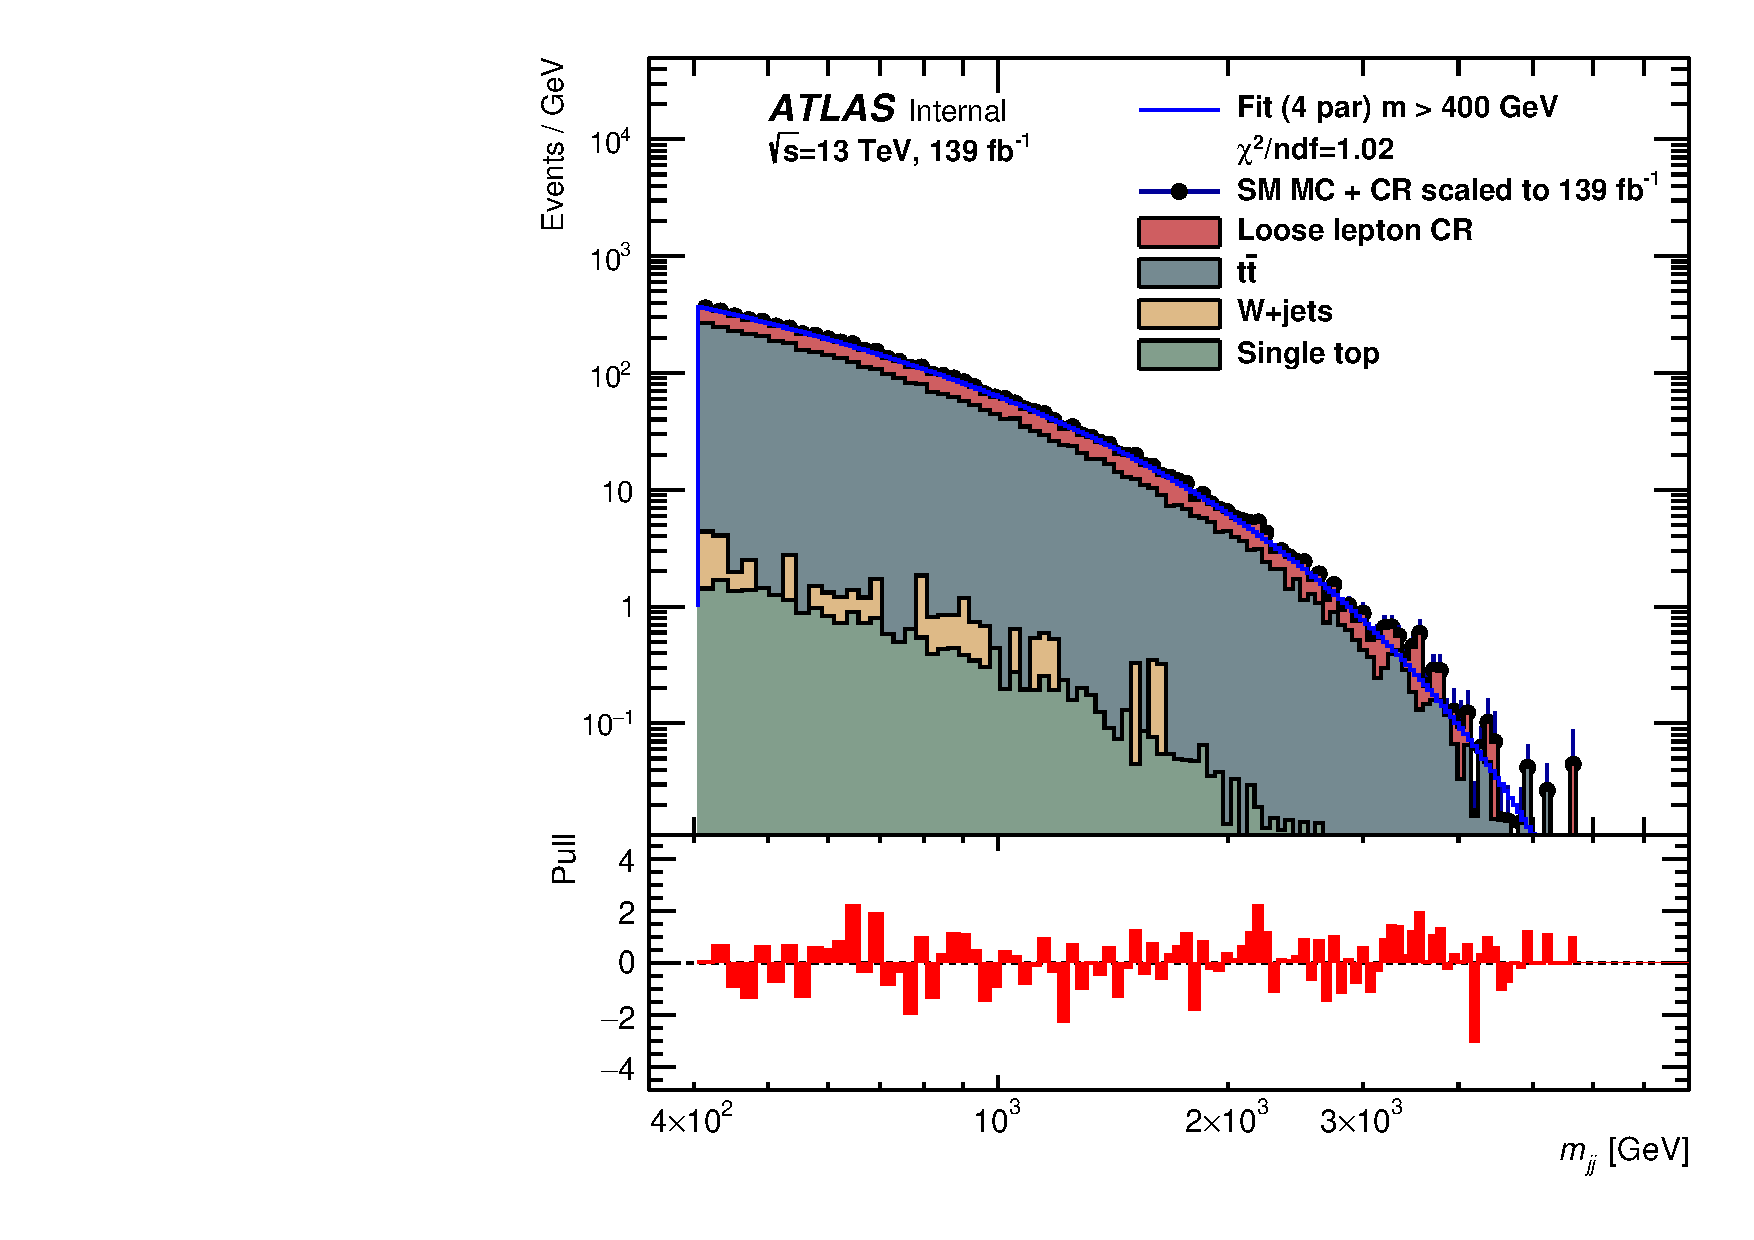
\includegraphics[scale=0.3]{figs/ch6/fit/variable_nosmooth/p4/1PB/output_SMMCplusCR_Mjj_p4.pdf}%
    \caption{\mjj \ using MC+LE-CR, p4}
    \end{subfigure}
    \hfill
    \begin{subfigure}[h]{0.4\linewidth}
    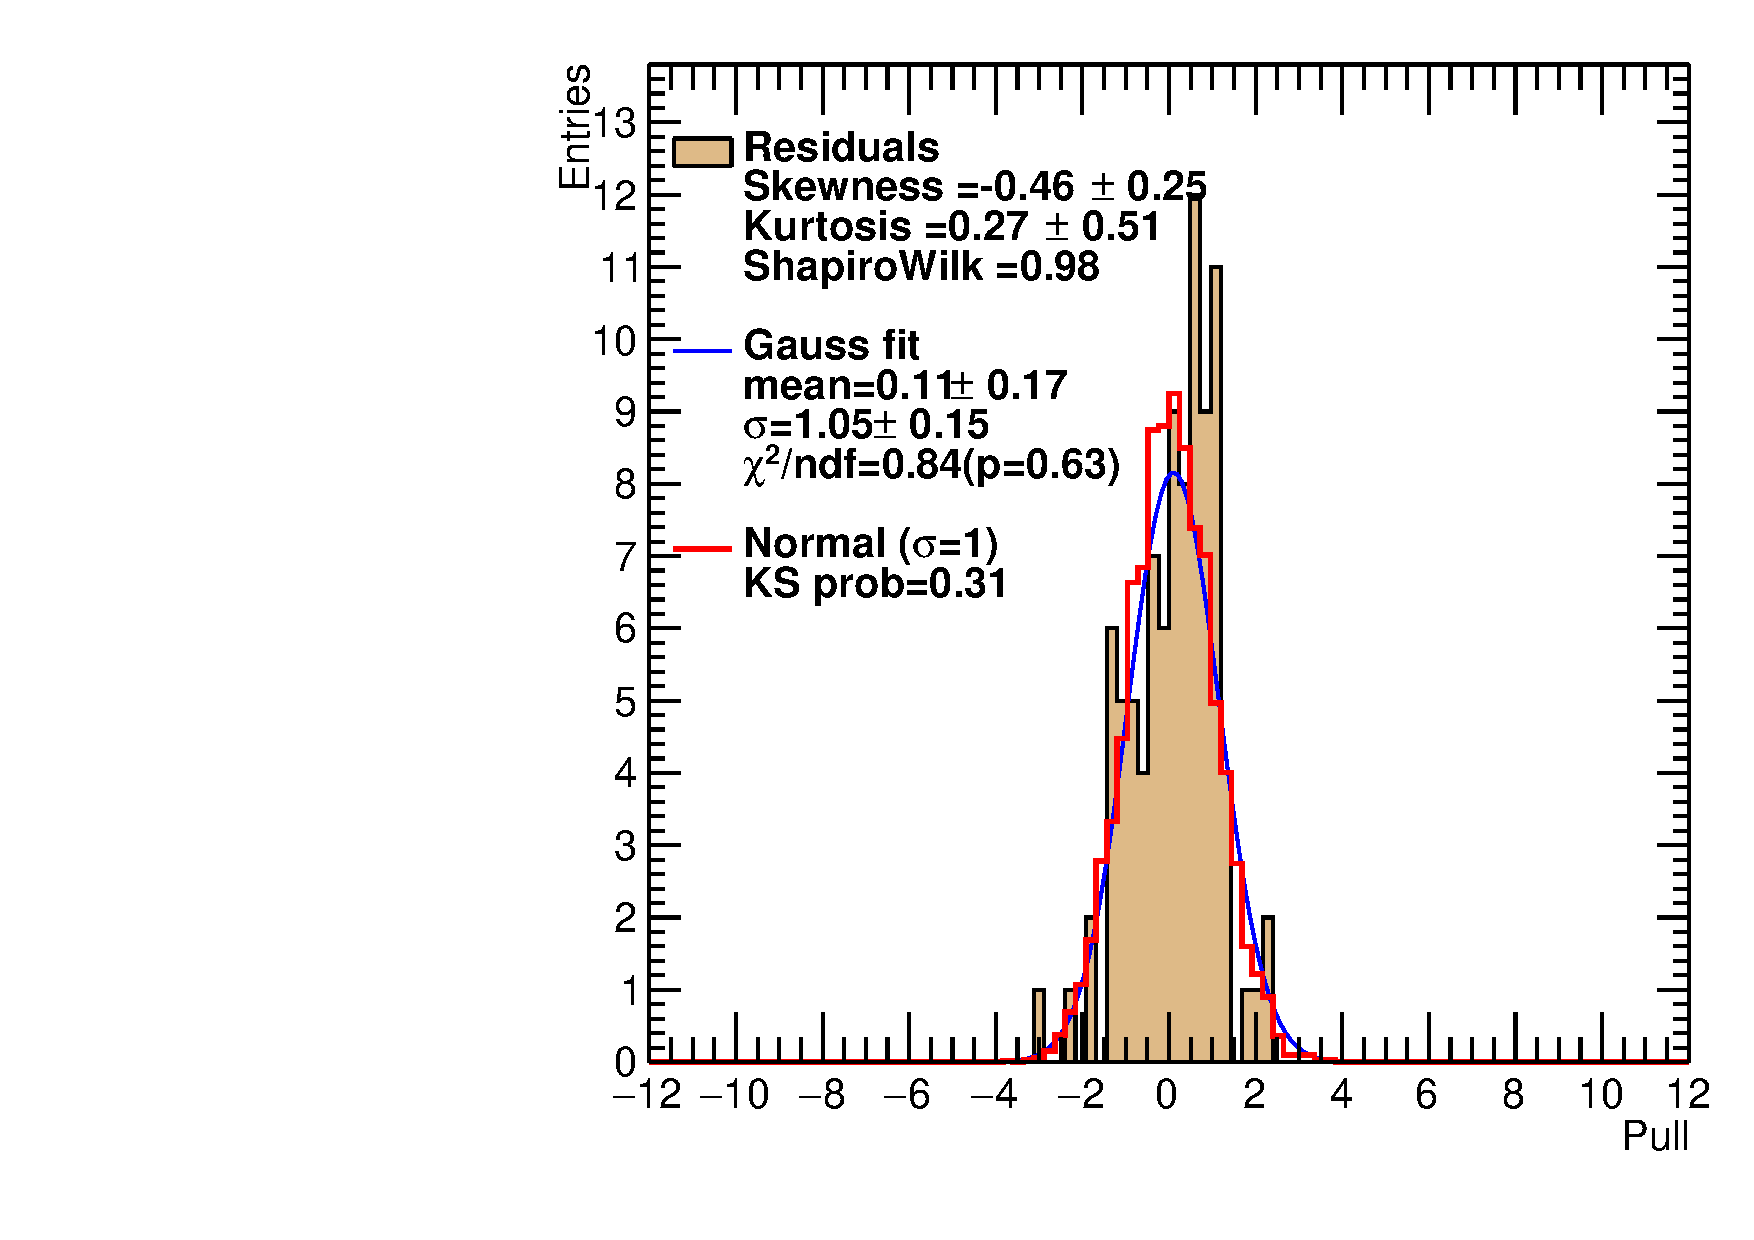
\includegraphics[scale=0.32]{figs/ch6/fit/variable_nosmooth/p4/1PB/pull_SMMCplusCR_Mjj_p4.pdf}%
    \caption{pulls of \mjj \ in p4}
    \end{subfigure}
    \hfill
    \begin{subfigure}[h]{0.38\linewidth}
    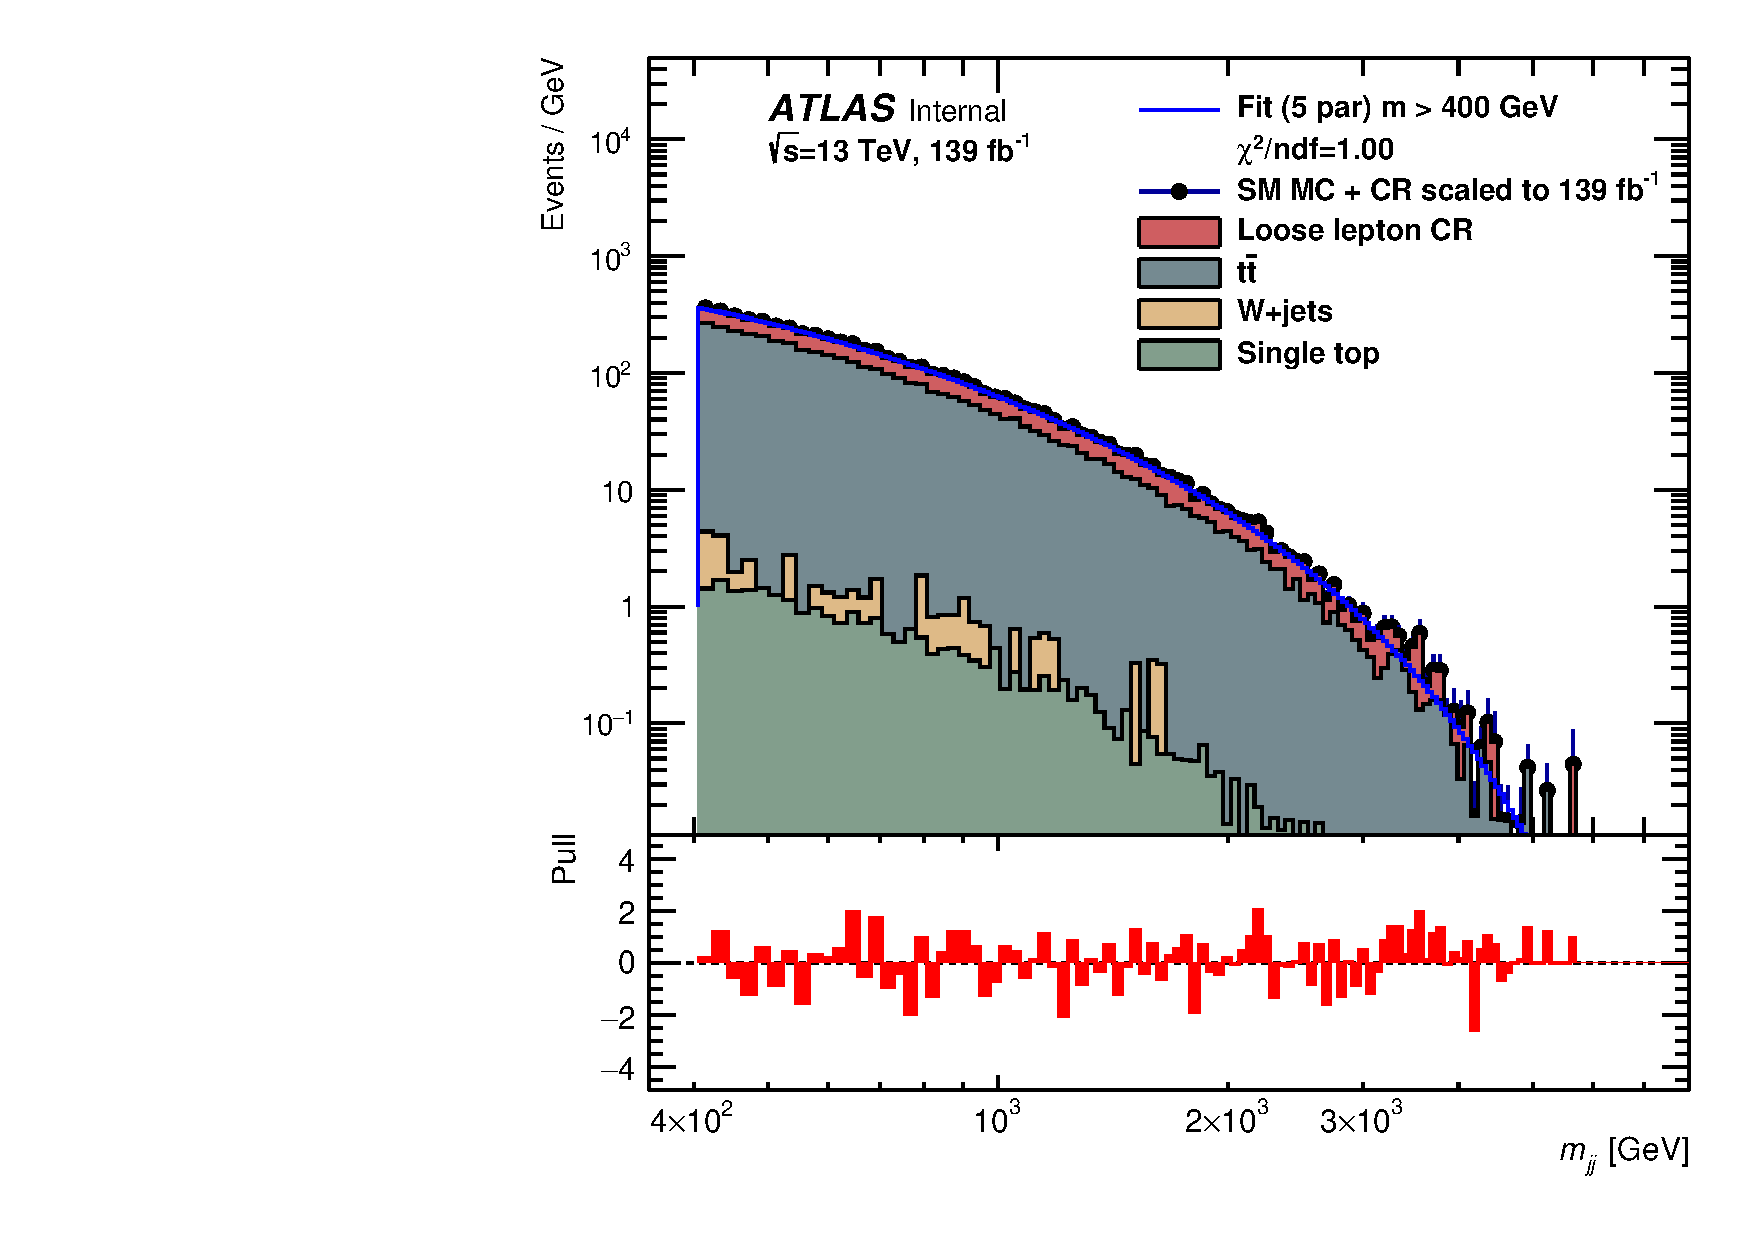
\includegraphics[scale=0.3]{figs/ch6/fit/variable_nosmooth/p5/1PB/output_SMMCplusCR_Mjj_p5.pdf}%
     \caption{\mjj \ using MC+LE-CR, p5}
     \end{subfigure}
     \hfill
    \begin{subfigure}[h]{0.4\linewidth}
    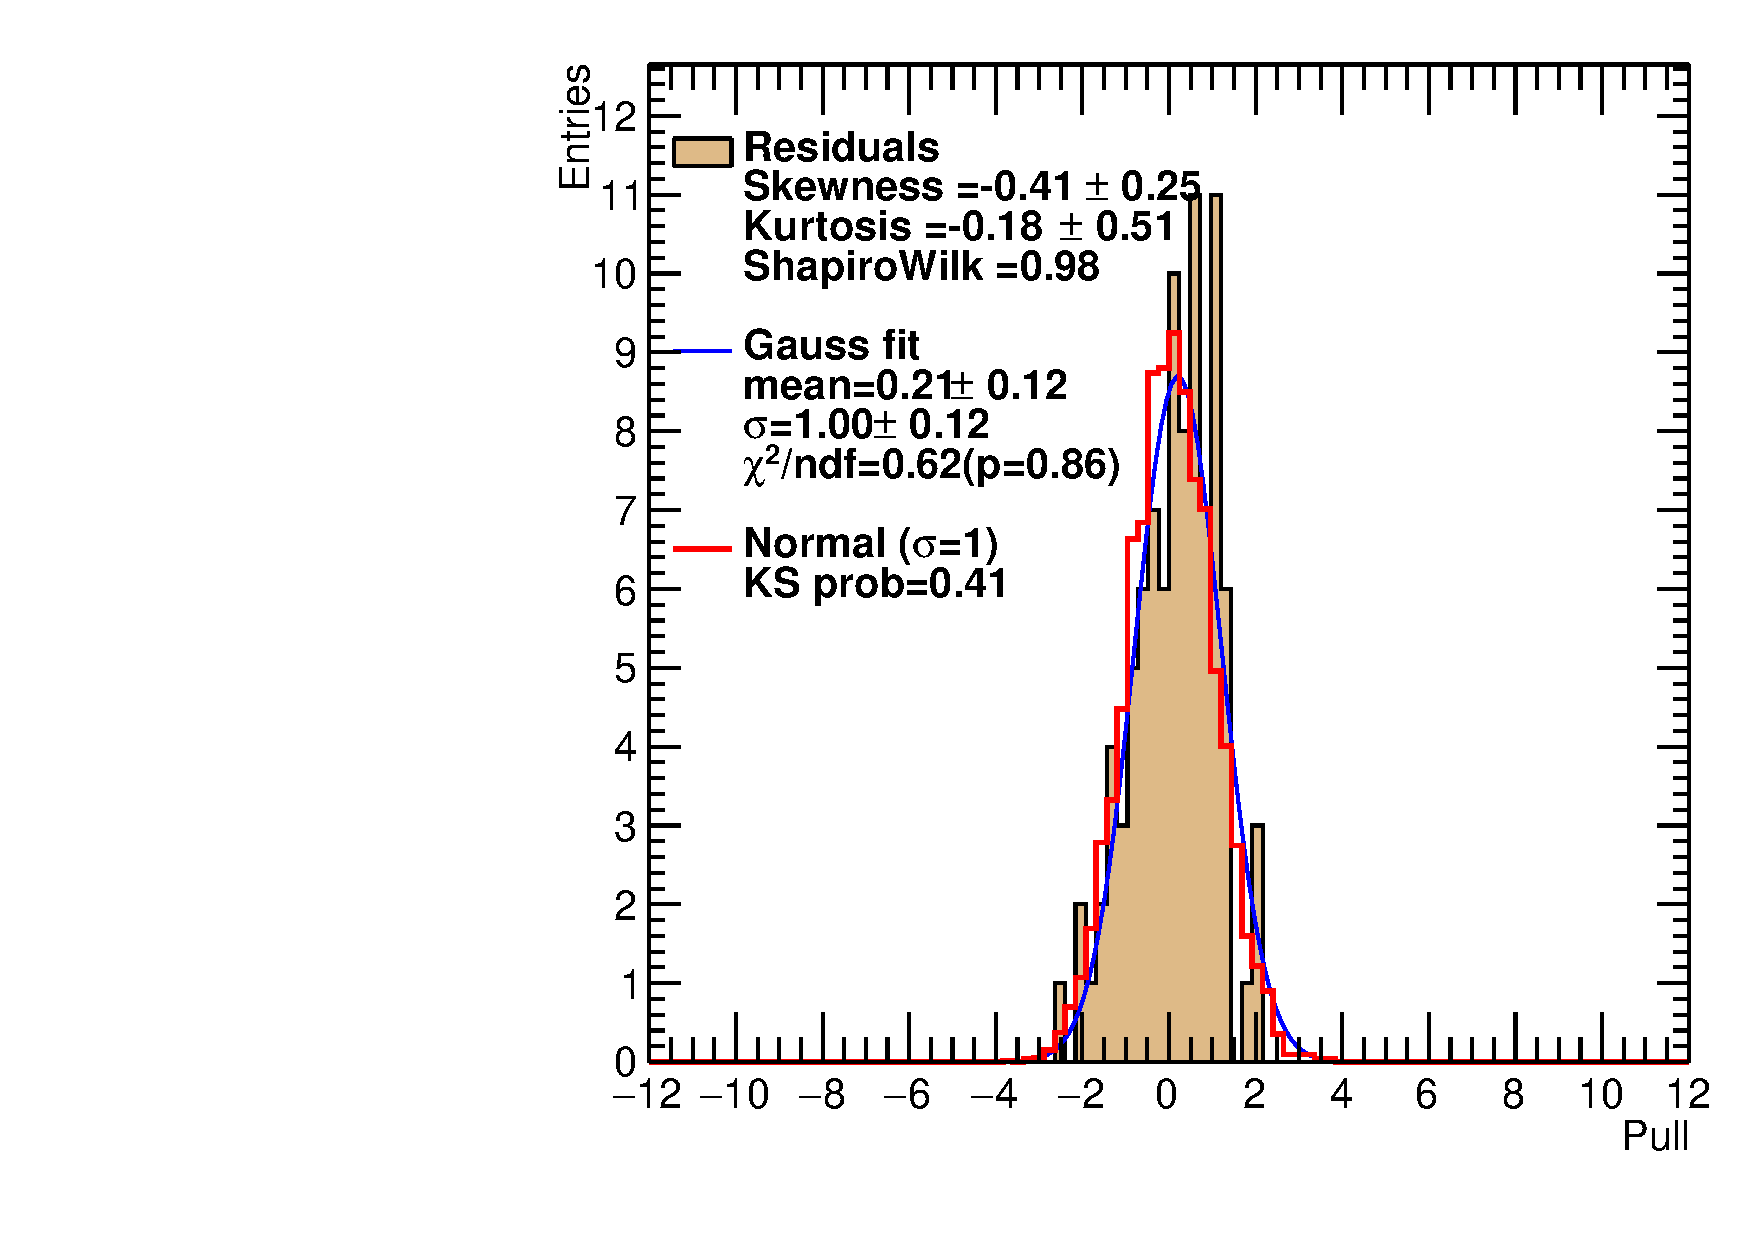
\includegraphics[scale=0.32]{figs/ch6/fit/variable_nosmooth/p5/1PB/pull_SMMCplusCR_Mjj_p5.pdf}%
    \caption{pulls of \mjj \ in p5}
    \end{subfigure}
    \caption{The \mjj \ invariant masses with the p4 and p5 fit functions in the BSM region after the 1 pb AR cut is applied. The MC processes are scaled to their cross sections, while the LE-CR is used to fill the missing event rate. Pulls shown on the right.}
\label{fig:mjj-fit-pulls-1pb}
\end{figure}

\newpage

\begin{figure}[ht]
    \centering
    \begin{subfigure}[h]{0.38\linewidth}
    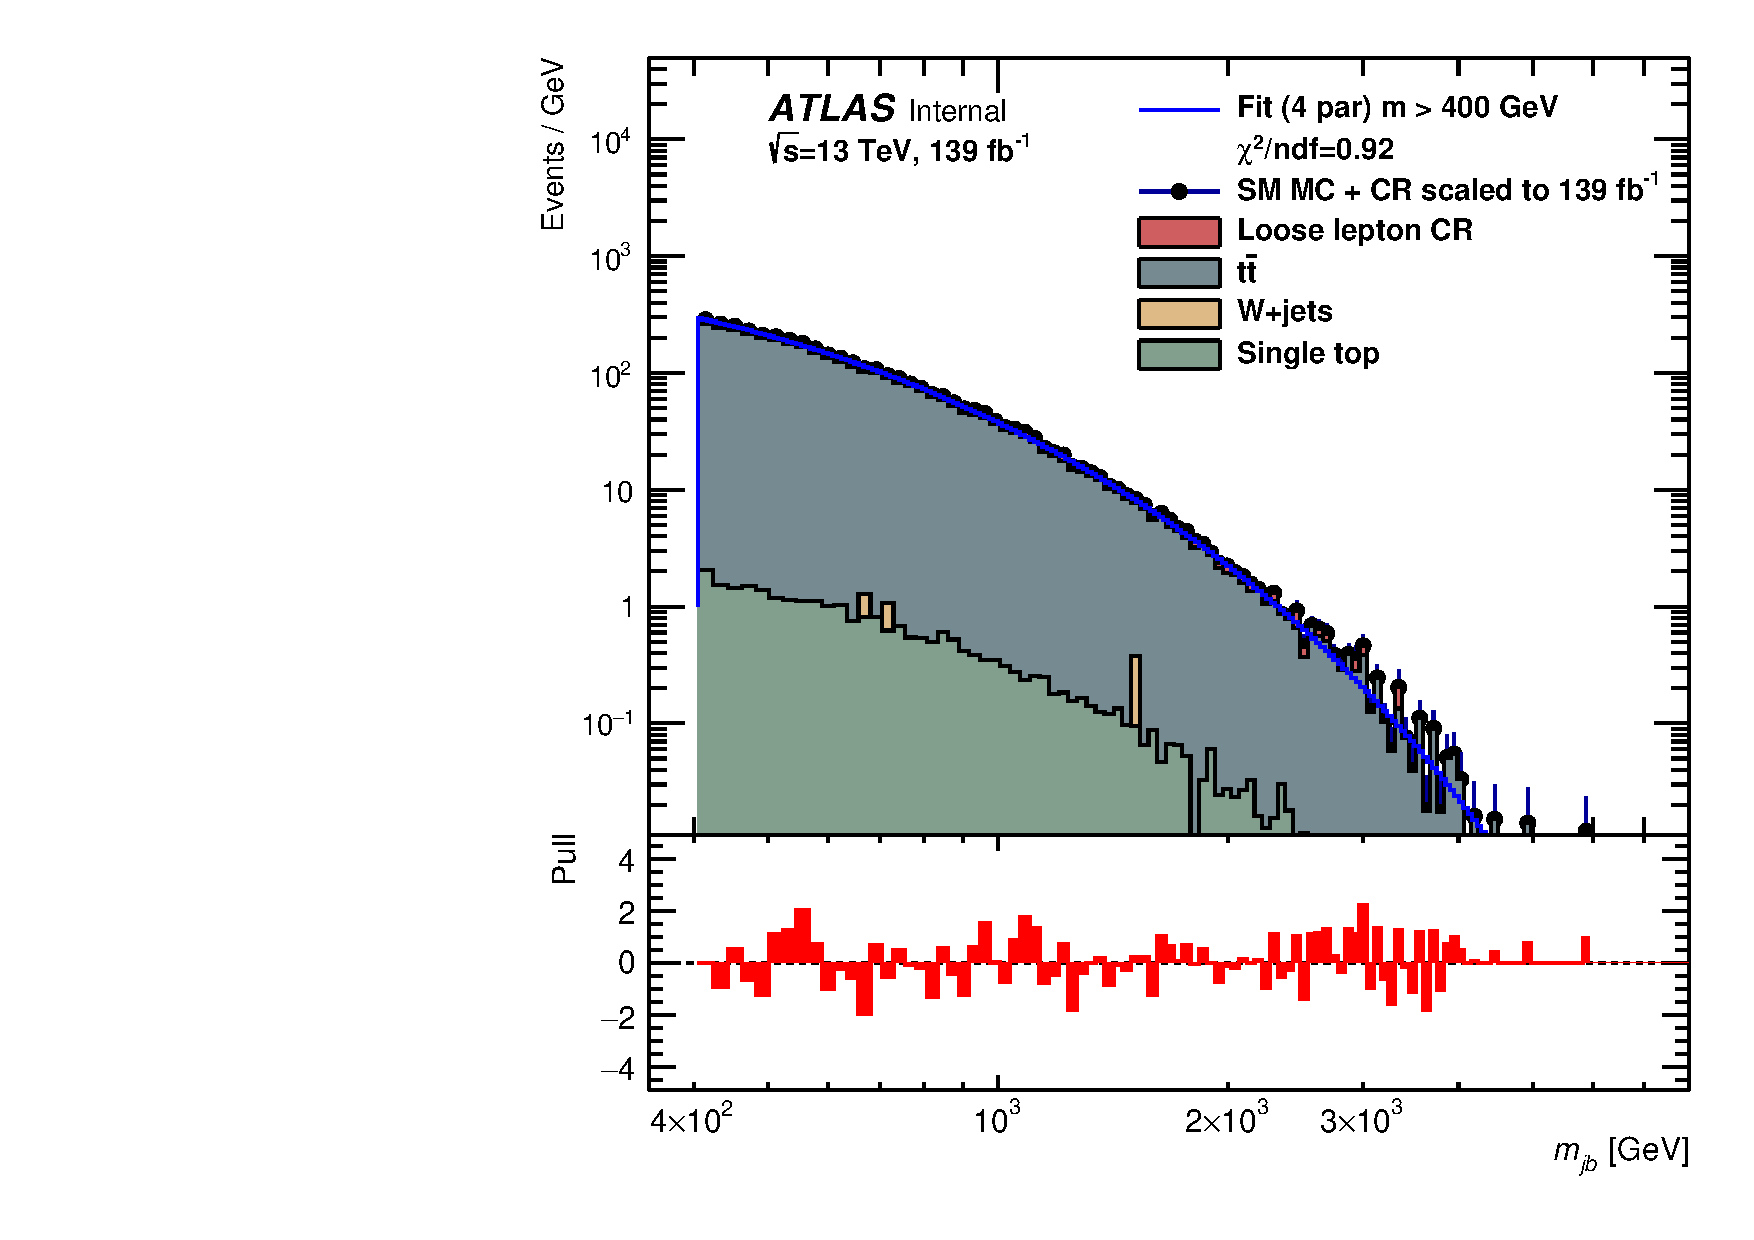
\includegraphics[scale=0.3]{figs/ch6/fit/variable_nosmooth/p4/1PB/output_SMMCplusCR_Mjb_p4.pdf}%
    \caption{\mjb \ using MC+LE-CR, p4}
    \end{subfigure}
    \hfill
    \begin{subfigure}[h]{0.4\linewidth}
    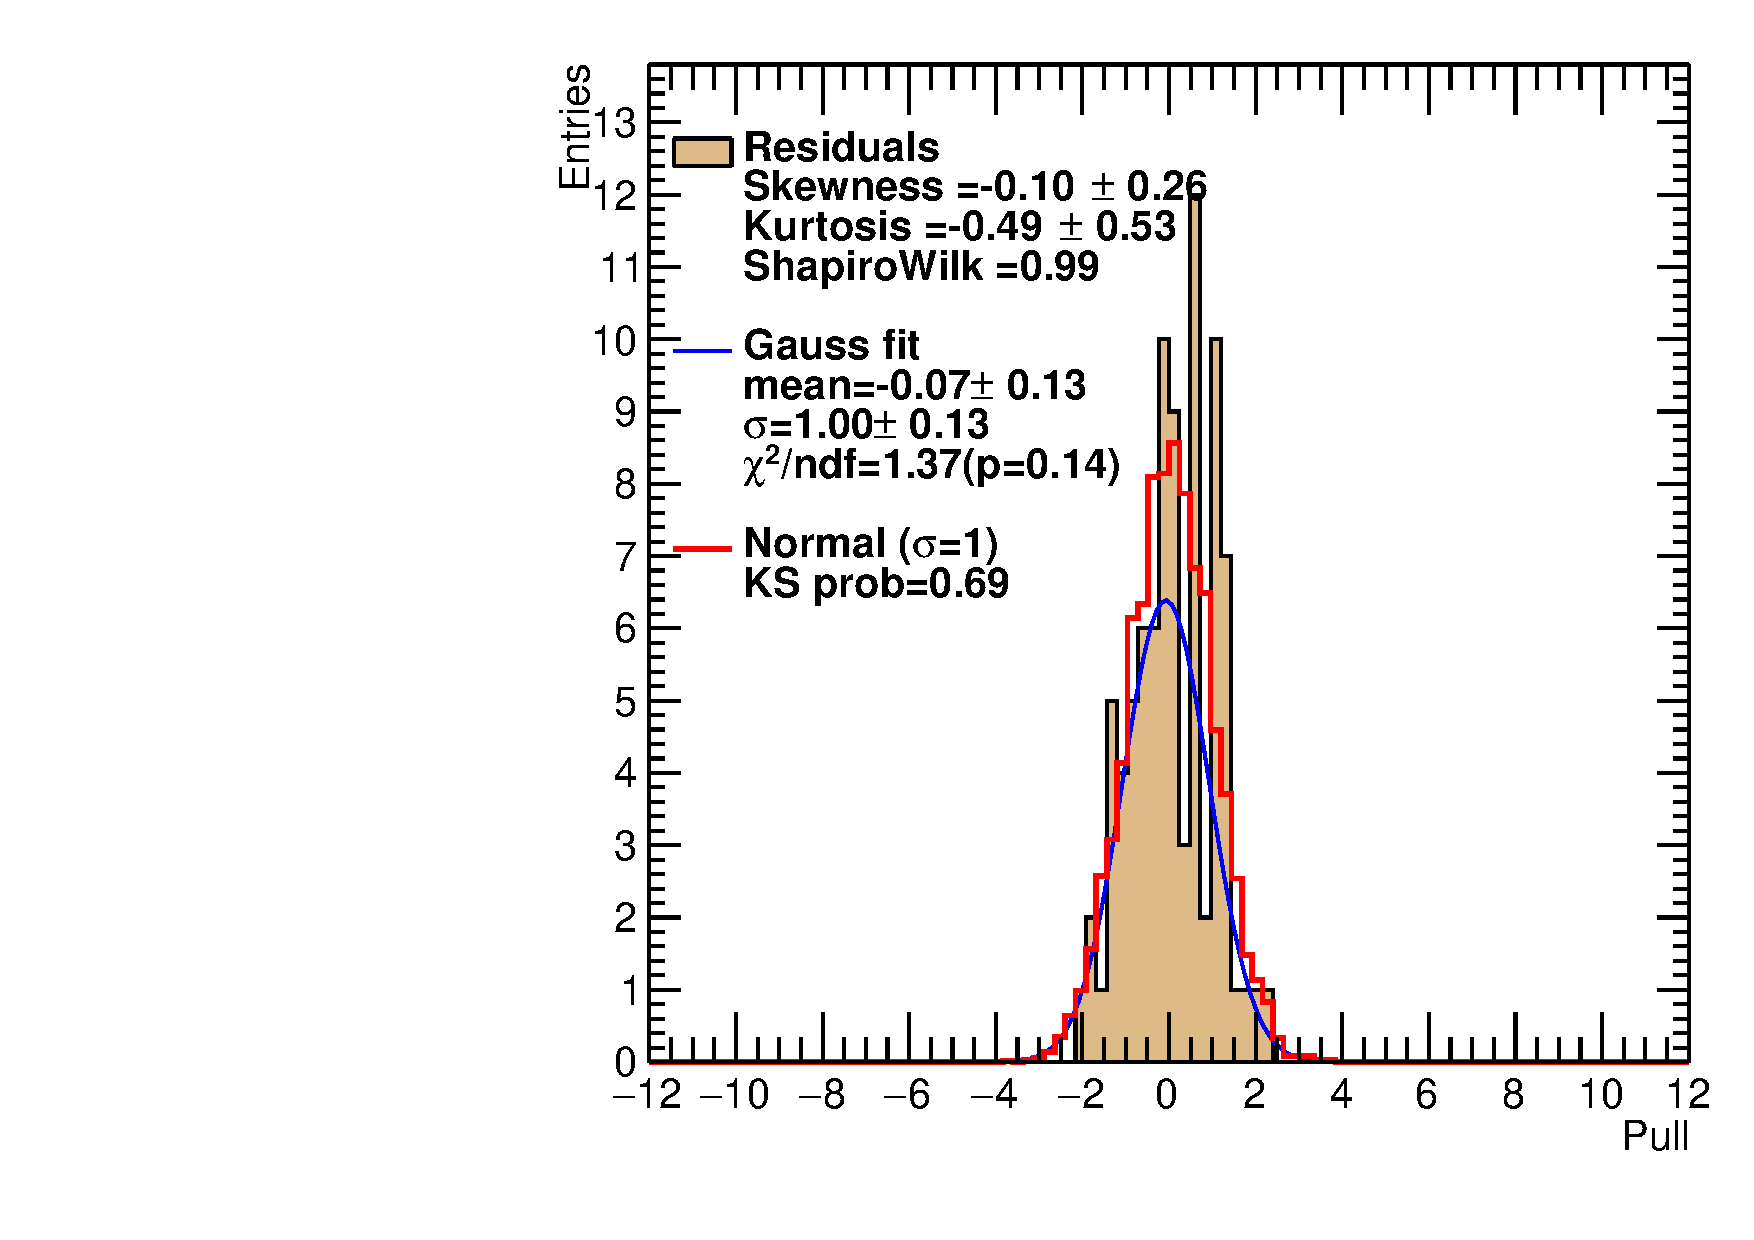
\includegraphics[scale=0.32]{figs/ch6/fit/variable_nosmooth/p4/1PB/pull_SMMCplusCR_Mjb_p4.pdf}%
    \caption{pulls of \mjb \ in p4}
    \end{subfigure}
    \hfill
    \begin{subfigure}[h]{0.38\linewidth}
    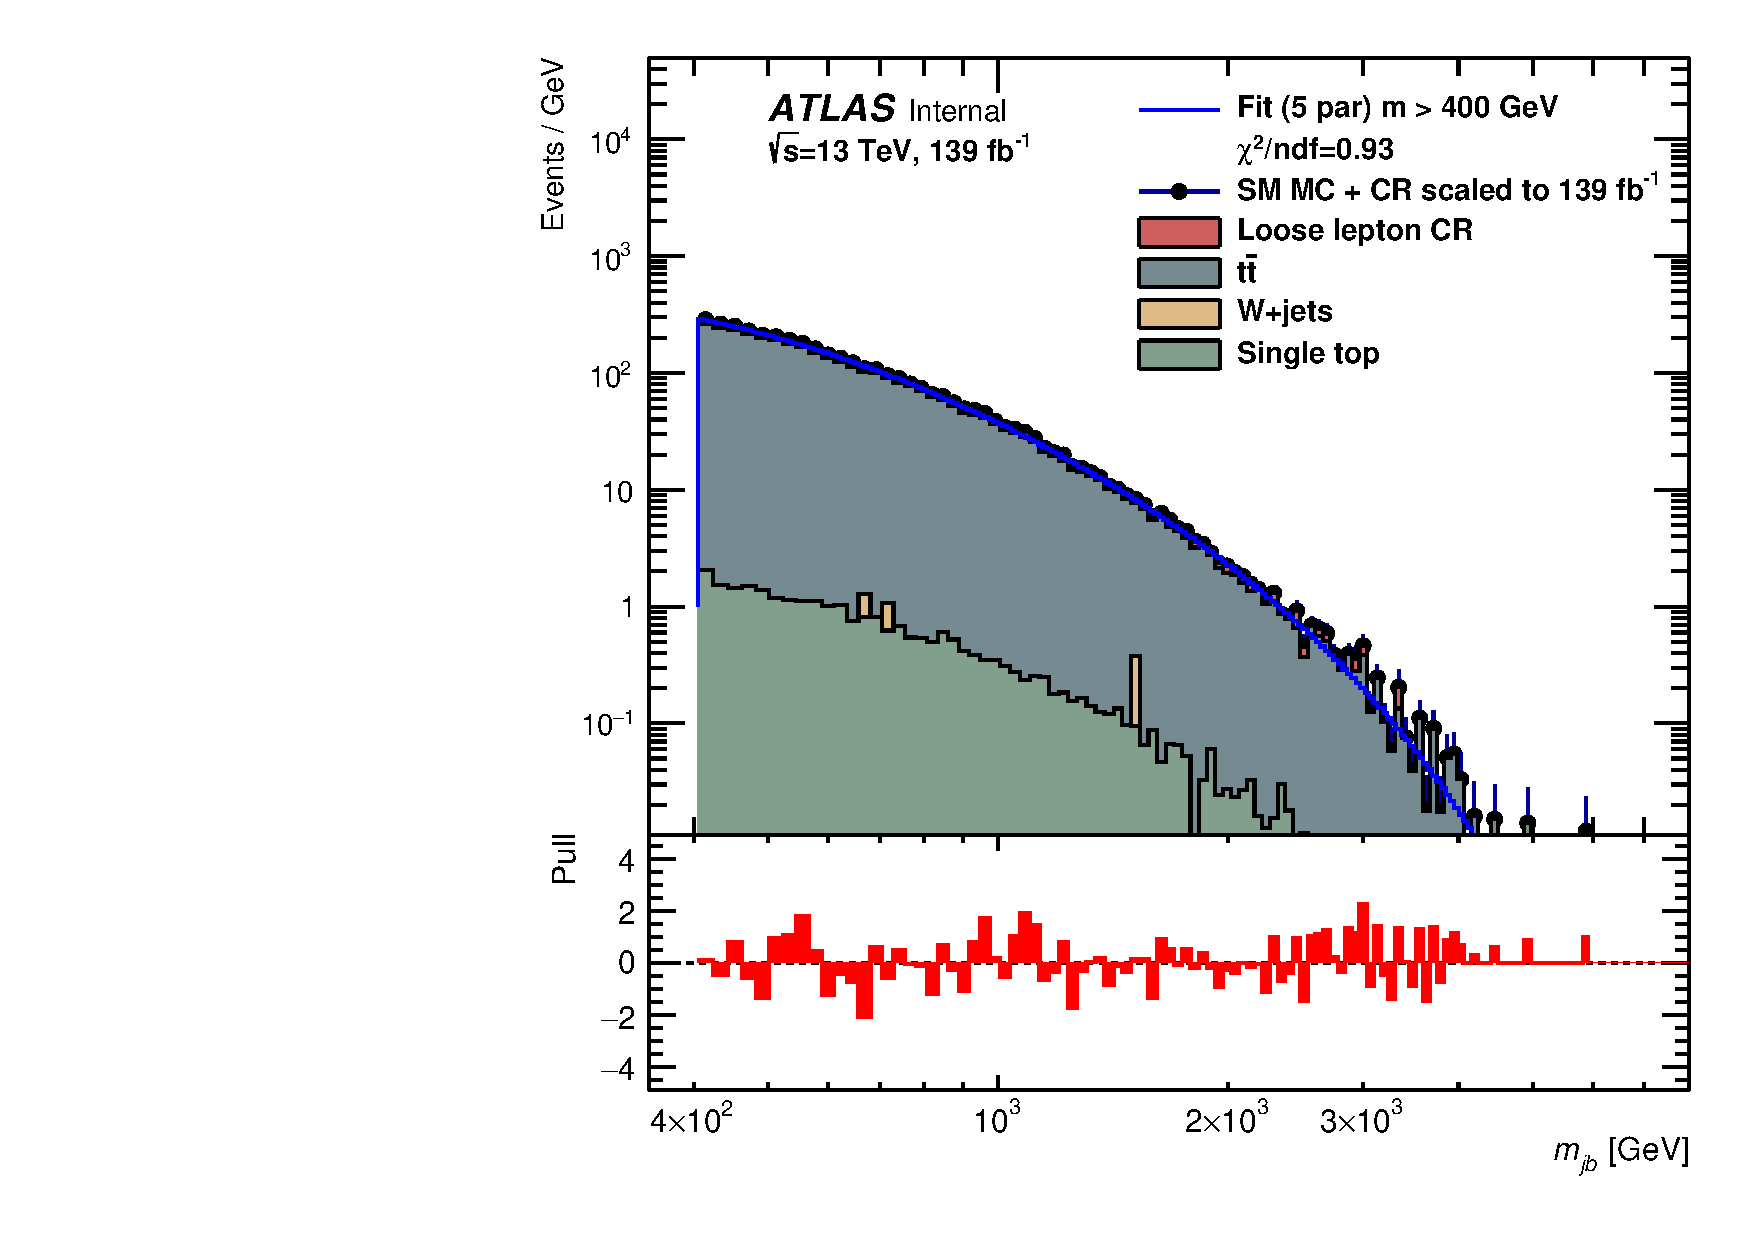
\includegraphics[scale=0.3]{figs/ch6/fit/variable_nosmooth/p5/1PB/output_SMMCplusCR_Mjb_p5.pdf}%
     \caption{\mjb \ using MC+LE-CR, p5}
     \end{subfigure}
     \hfill
    \begin{subfigure}[h]{0.4\linewidth}
    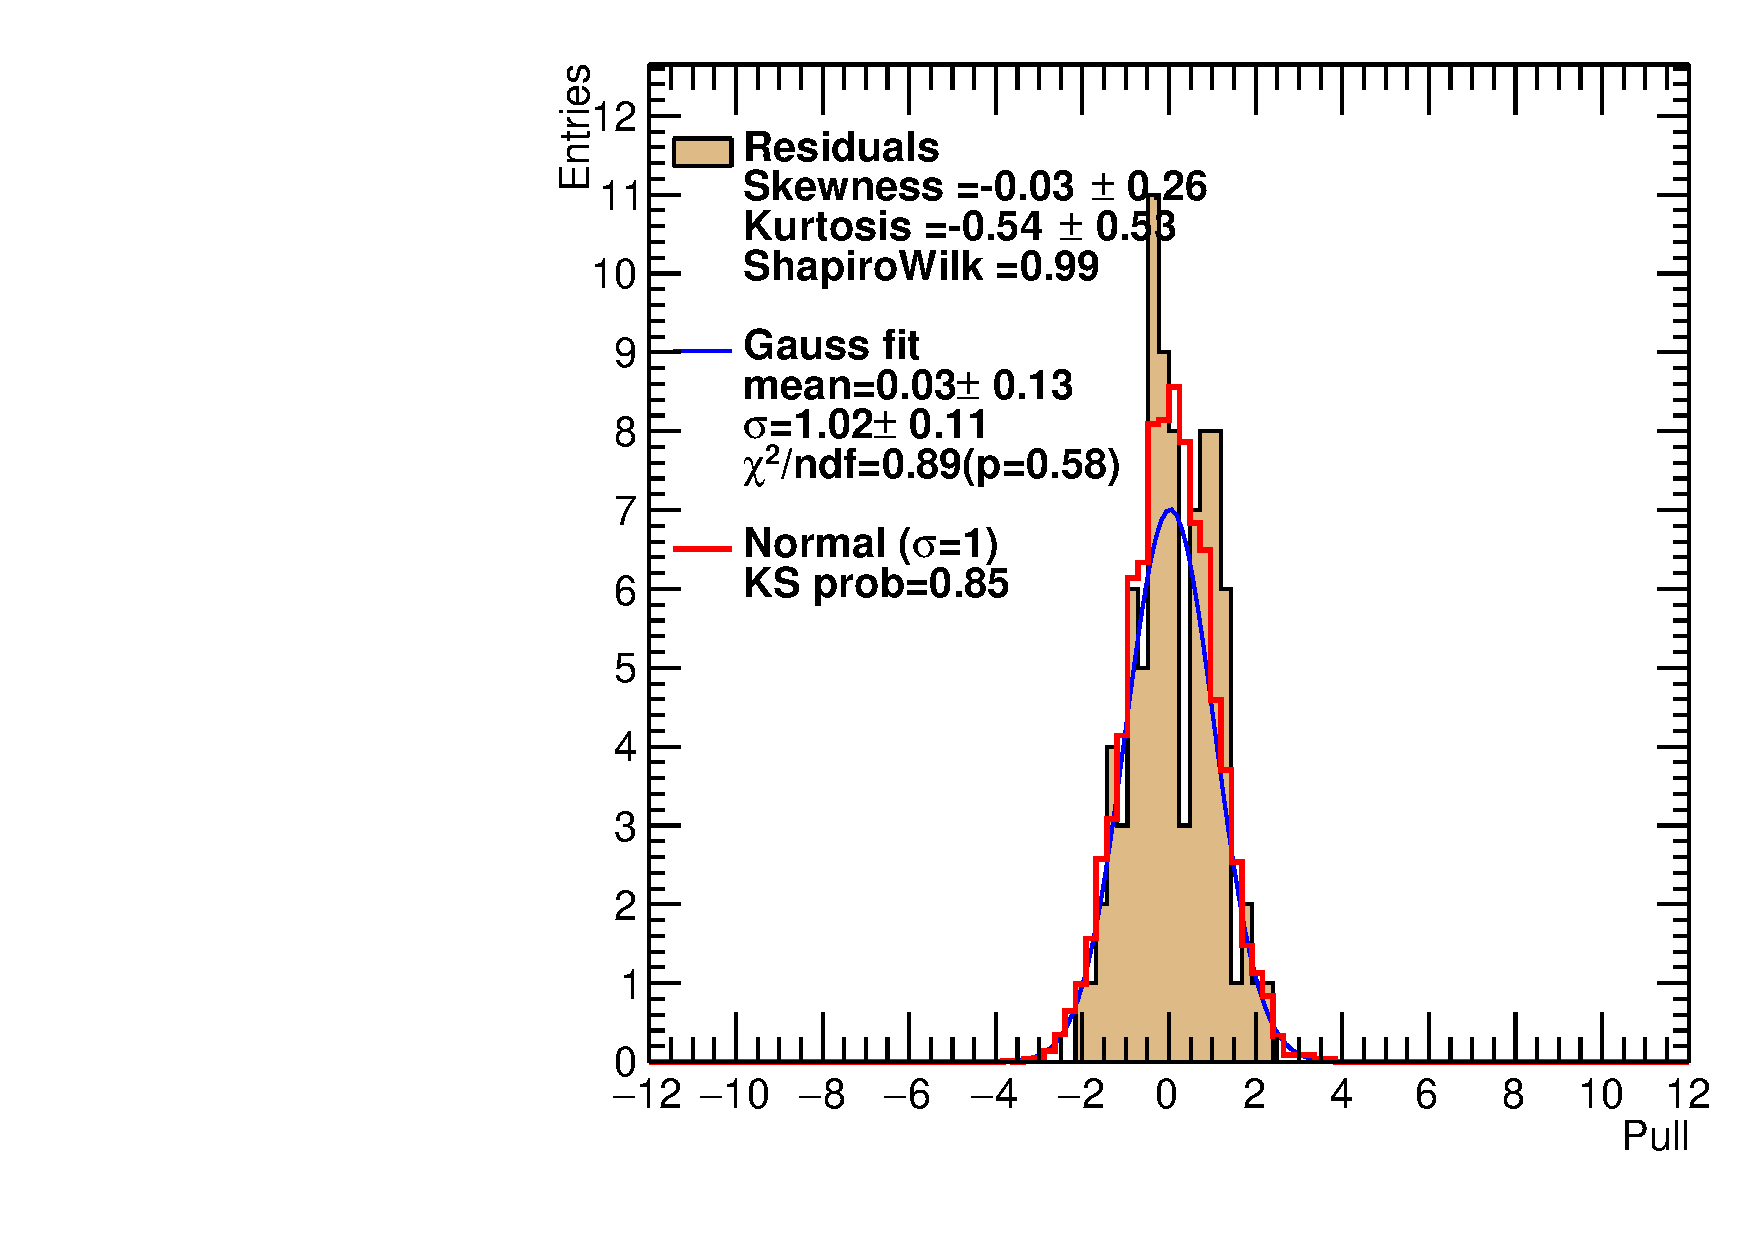
\includegraphics[scale=0.32]{figs/ch6/fit/variable_nosmooth/p5/1PB/pull_SMMCplusCR_Mjb_p5.pdf}%
    \caption{pulls of \mjb \ in p5}
    \end{subfigure}
    \caption{The \mjb \ invariant masses with the p4 and p5 fit functions in the BSM region after the 1 pb AR cut is applied. The MC processes are scaled to their cross sections, while the LE-CR is used to fill the missing event rate. Pulls shown on the right.}
\label{fig:mjb-fit-pulls-1pb}
\end{figure}

\newpage

\begin{figure}[ht]
    \centering
    \begin{subfigure}[h]{0.38\linewidth}
    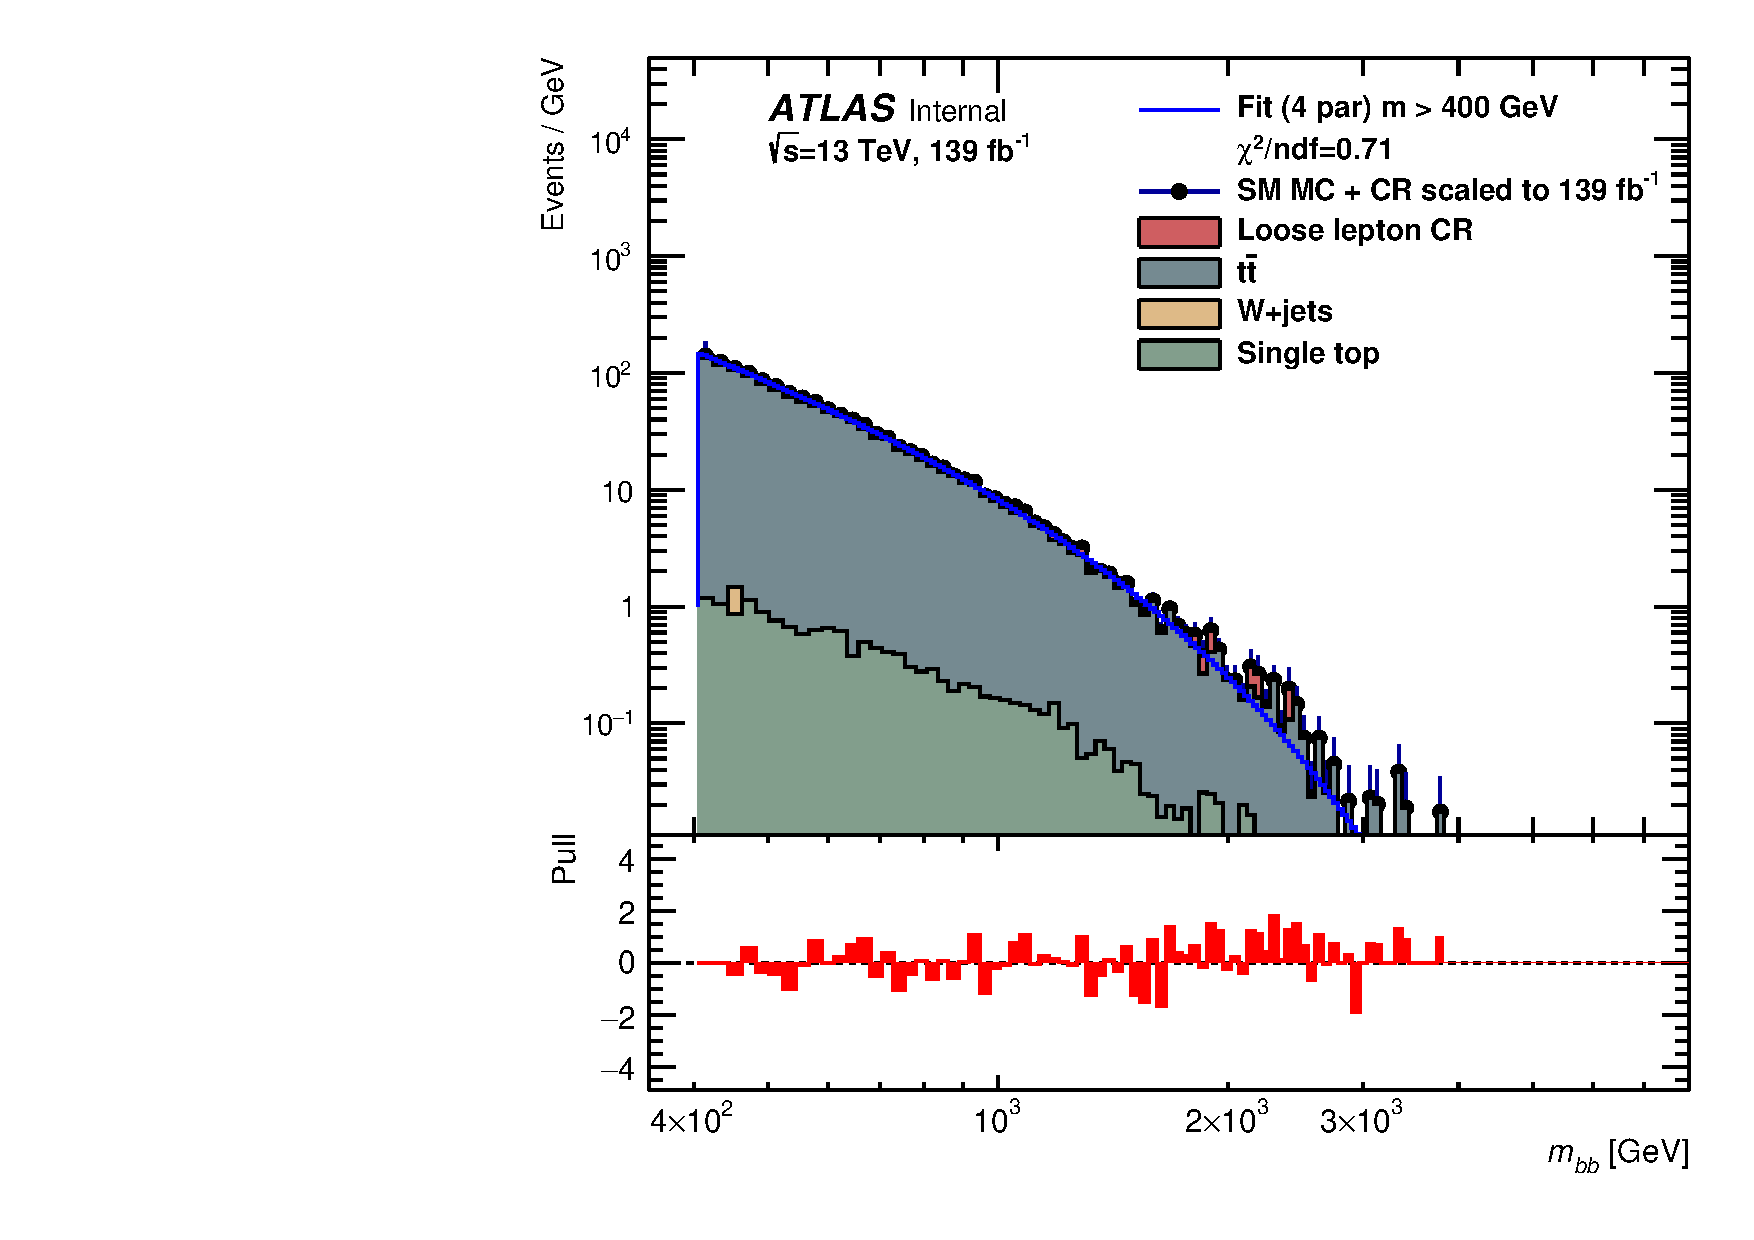
\includegraphics[scale=0.3]{figs/ch6/fit/variable_nosmooth/p4/1PB/output_SMMCplusCR_Mbb_p4.pdf}%
    \caption{\mbb \ using MC+LE-CR, p4}
    \end{subfigure}
    \hfill
    \begin{subfigure}[h]{0.4\linewidth}
    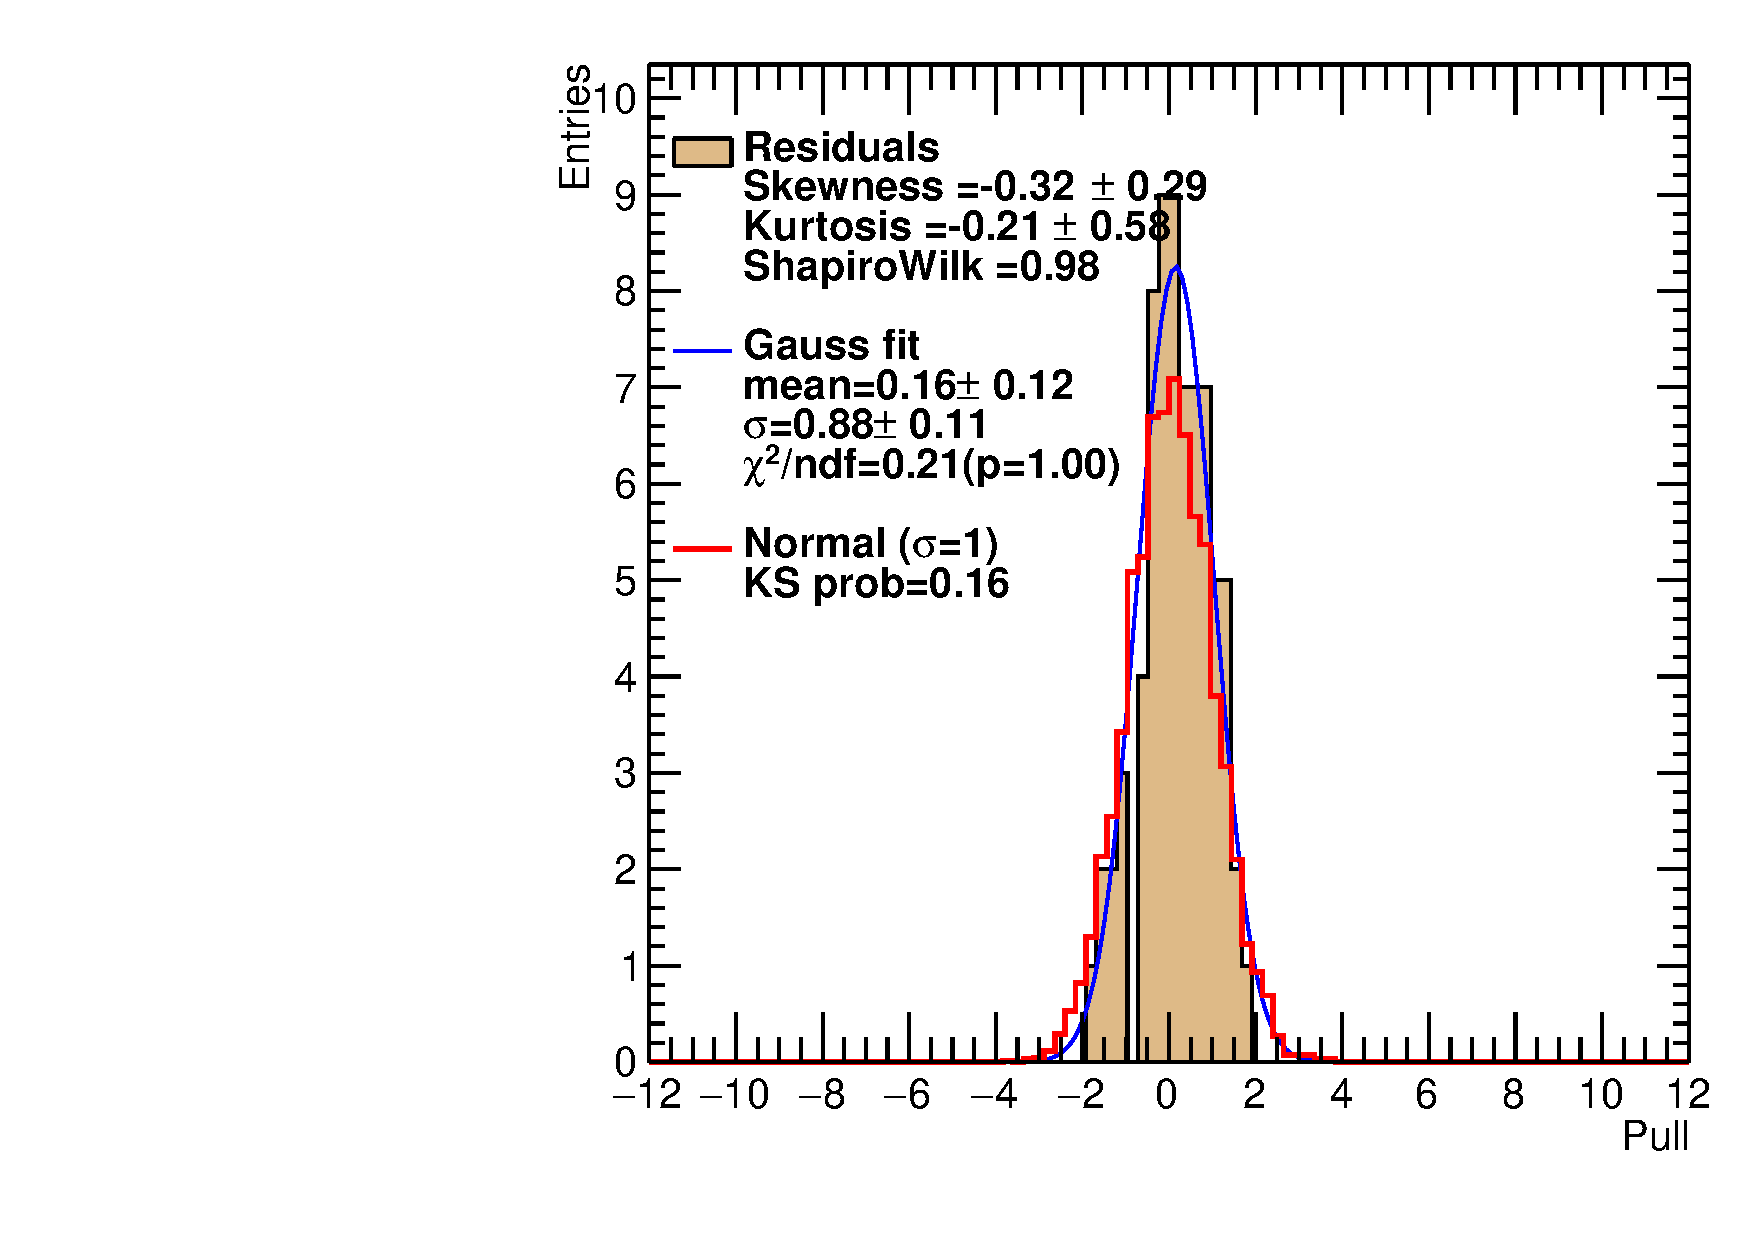
\includegraphics[scale=0.32]{figs/ch6/fit/variable_nosmooth/p4/1PB/pull_SMMCplusCR_Mbb_p4.pdf}%
    \caption{pulls of \mbb \ in p4}
    \end{subfigure}
    \hfill
    \begin{subfigure}[h]{0.38\linewidth}
    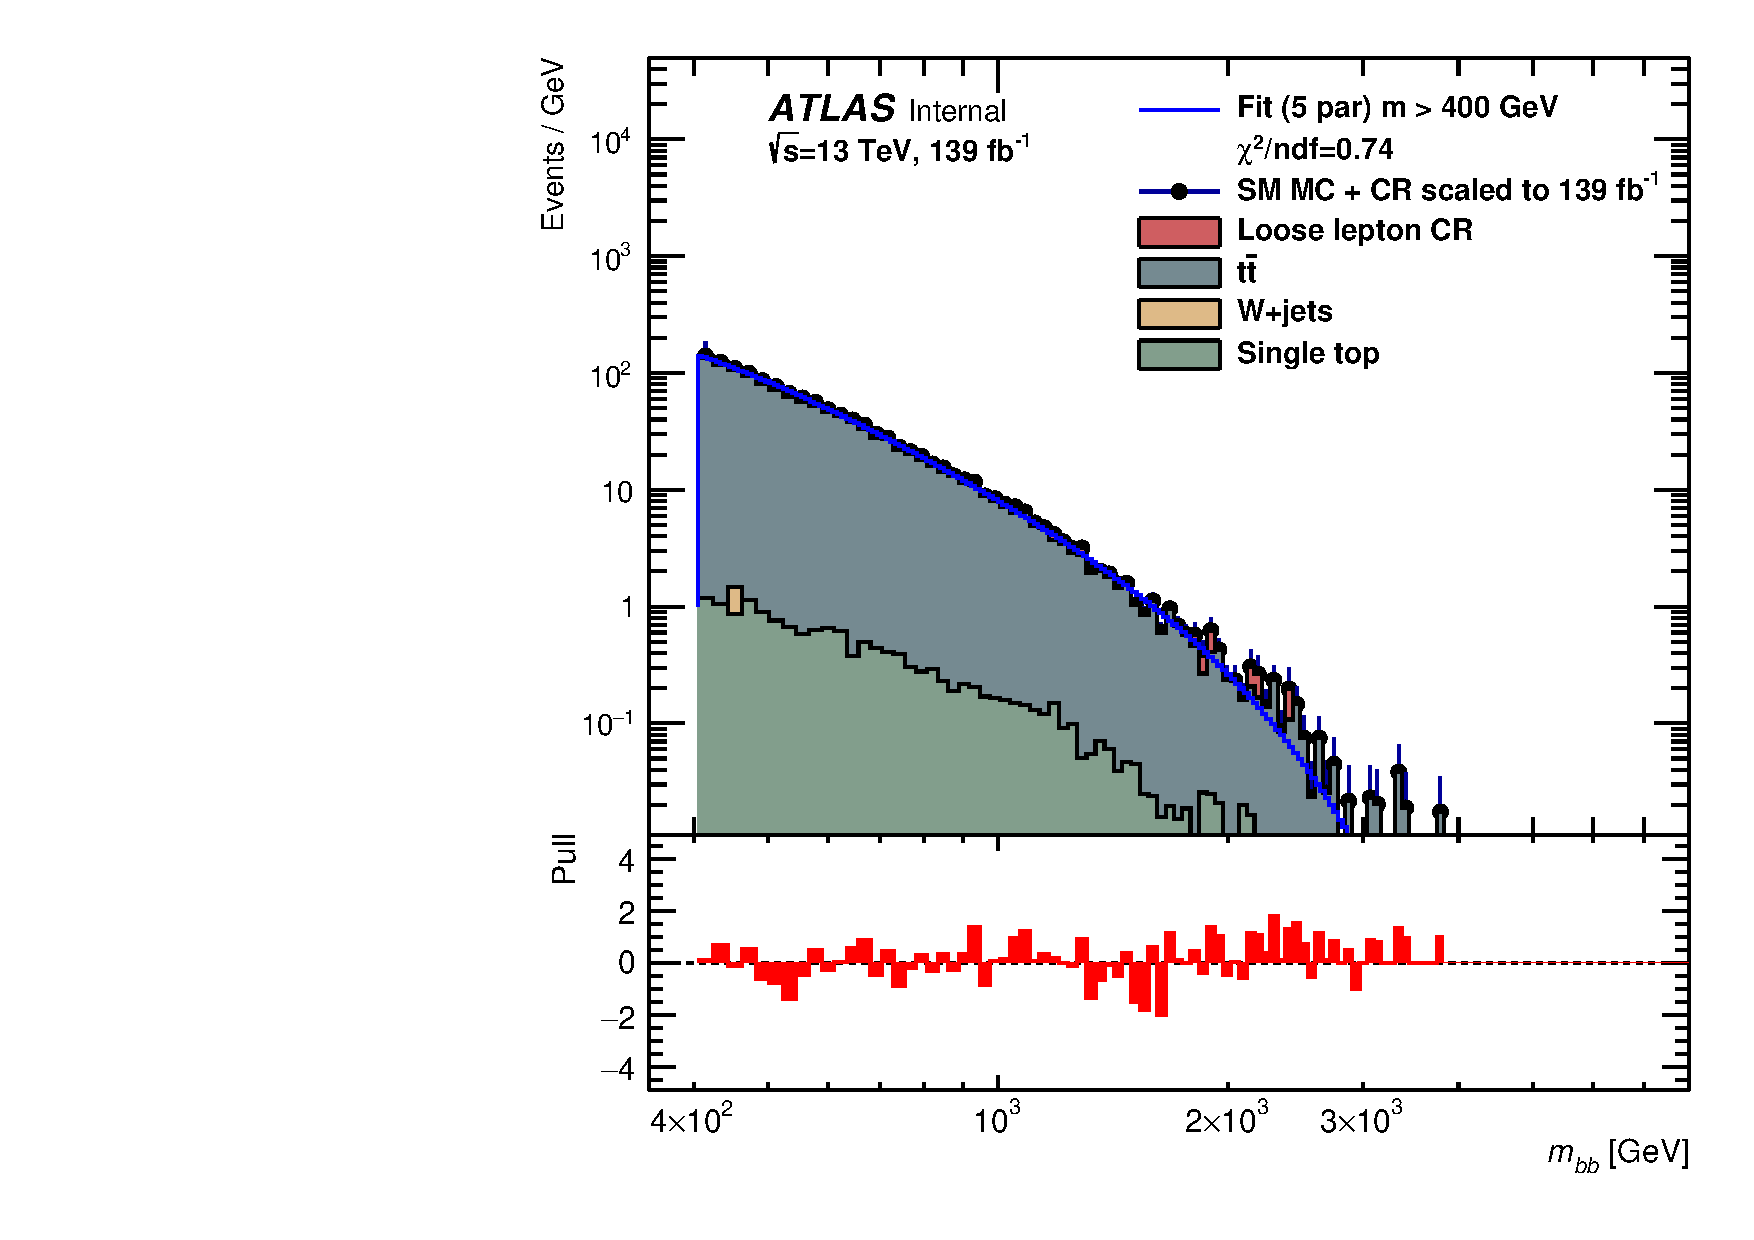
\includegraphics[scale=0.3]{figs/ch6/fit/variable_nosmooth/p5/1PB/output_SMMCplusCR_Mbb_p5.pdf}%
     \caption{\mbb \ using MC+LE-CR, p5}
     \end{subfigure}
     \hfill
    \begin{subfigure}[h]{0.4\linewidth}
    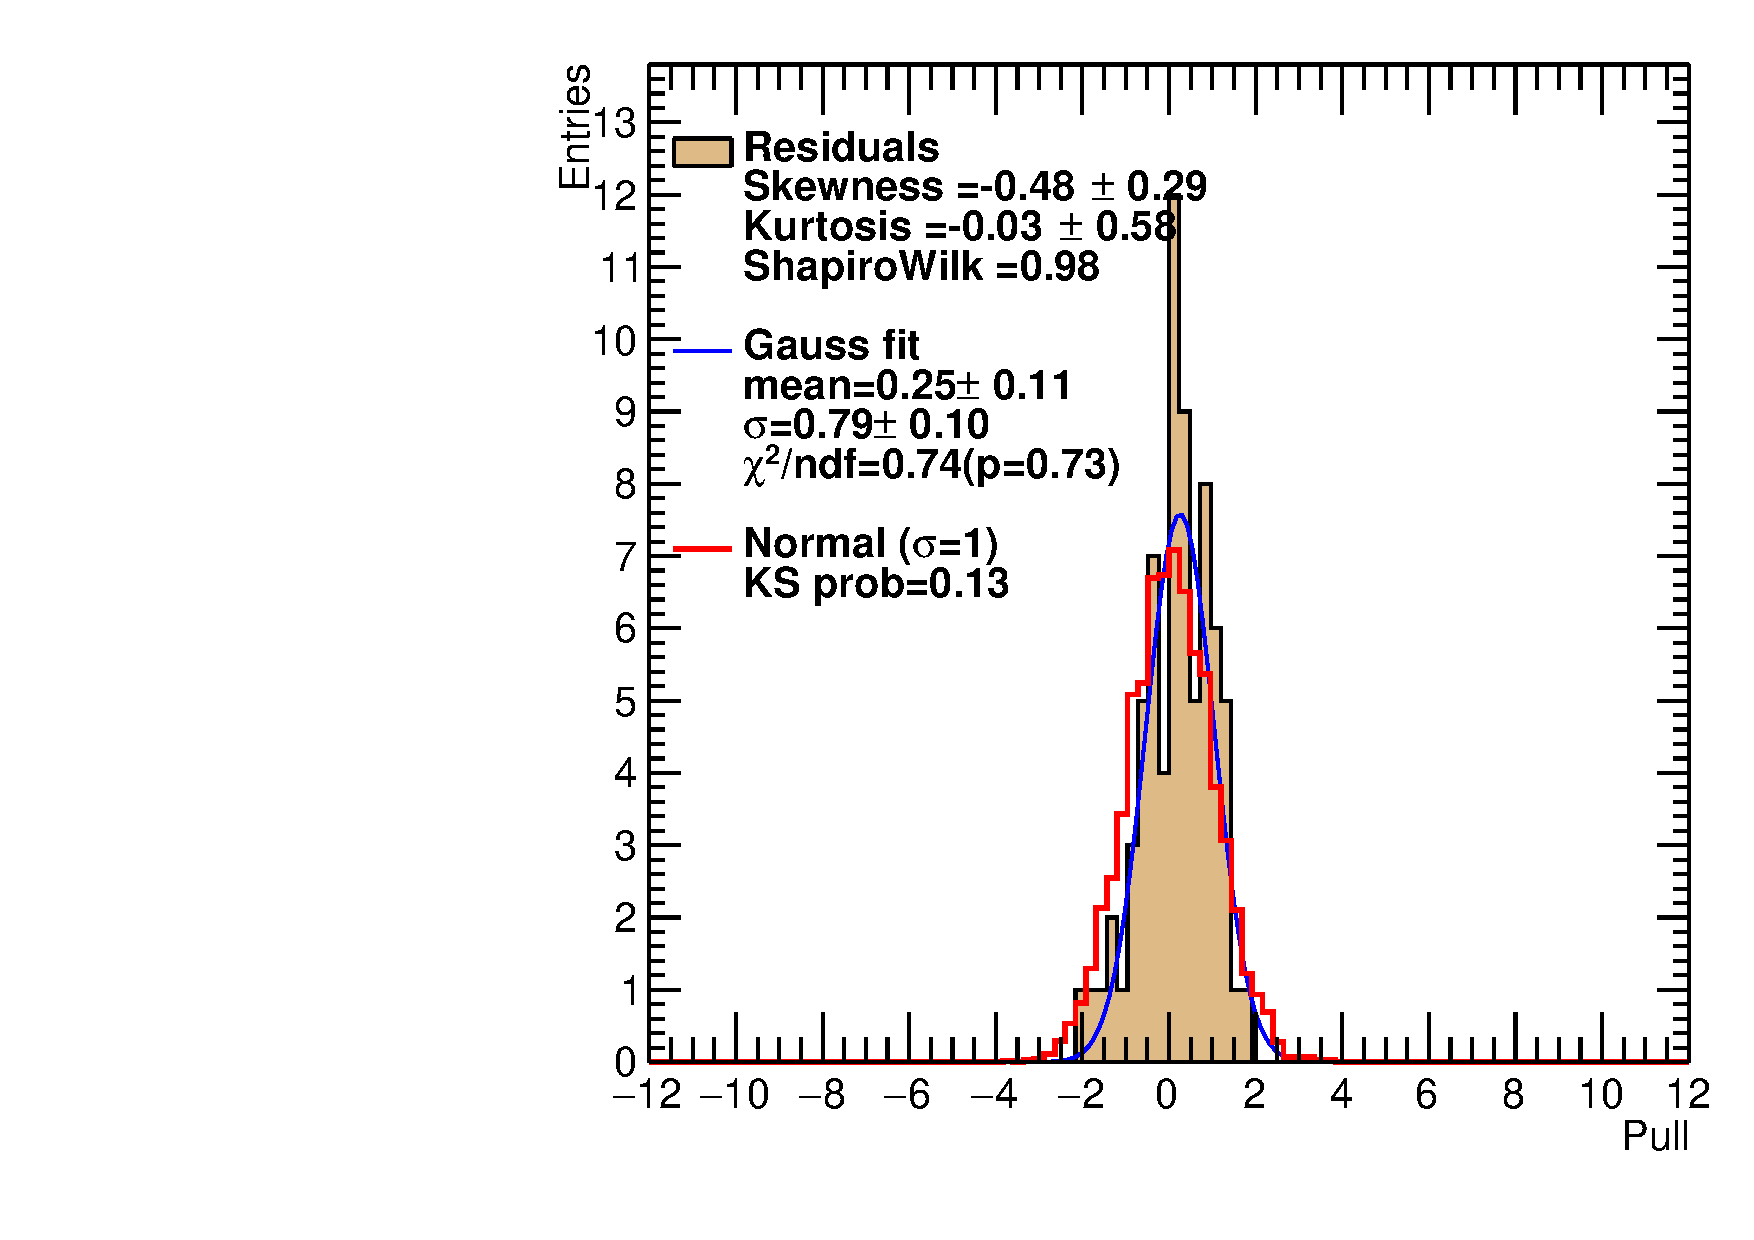
\includegraphics[scale=0.32]{figs/ch6/fit/variable_nosmooth/p5/1PB/pull_SMMCplusCR_Mbb_p5.pdf}%
    \caption{pulls of \mbb \ in p5}
    \end{subfigure}
    \caption{The \mbb \ invariant masses with the p4 and p5 fit functions in the BSM region after the 1 pb AR cut is applied. The MC processes are scaled to their cross sections, while the LE-CR is used to fill the missing event rate. Pulls shown on the right.}
\label{fig:mbb-fit-pulls-1pb}
\end{figure}

\newpage

\begin{figure}[ht]
    \centering
    \begin{subfigure}[h]{0.38\linewidth}
    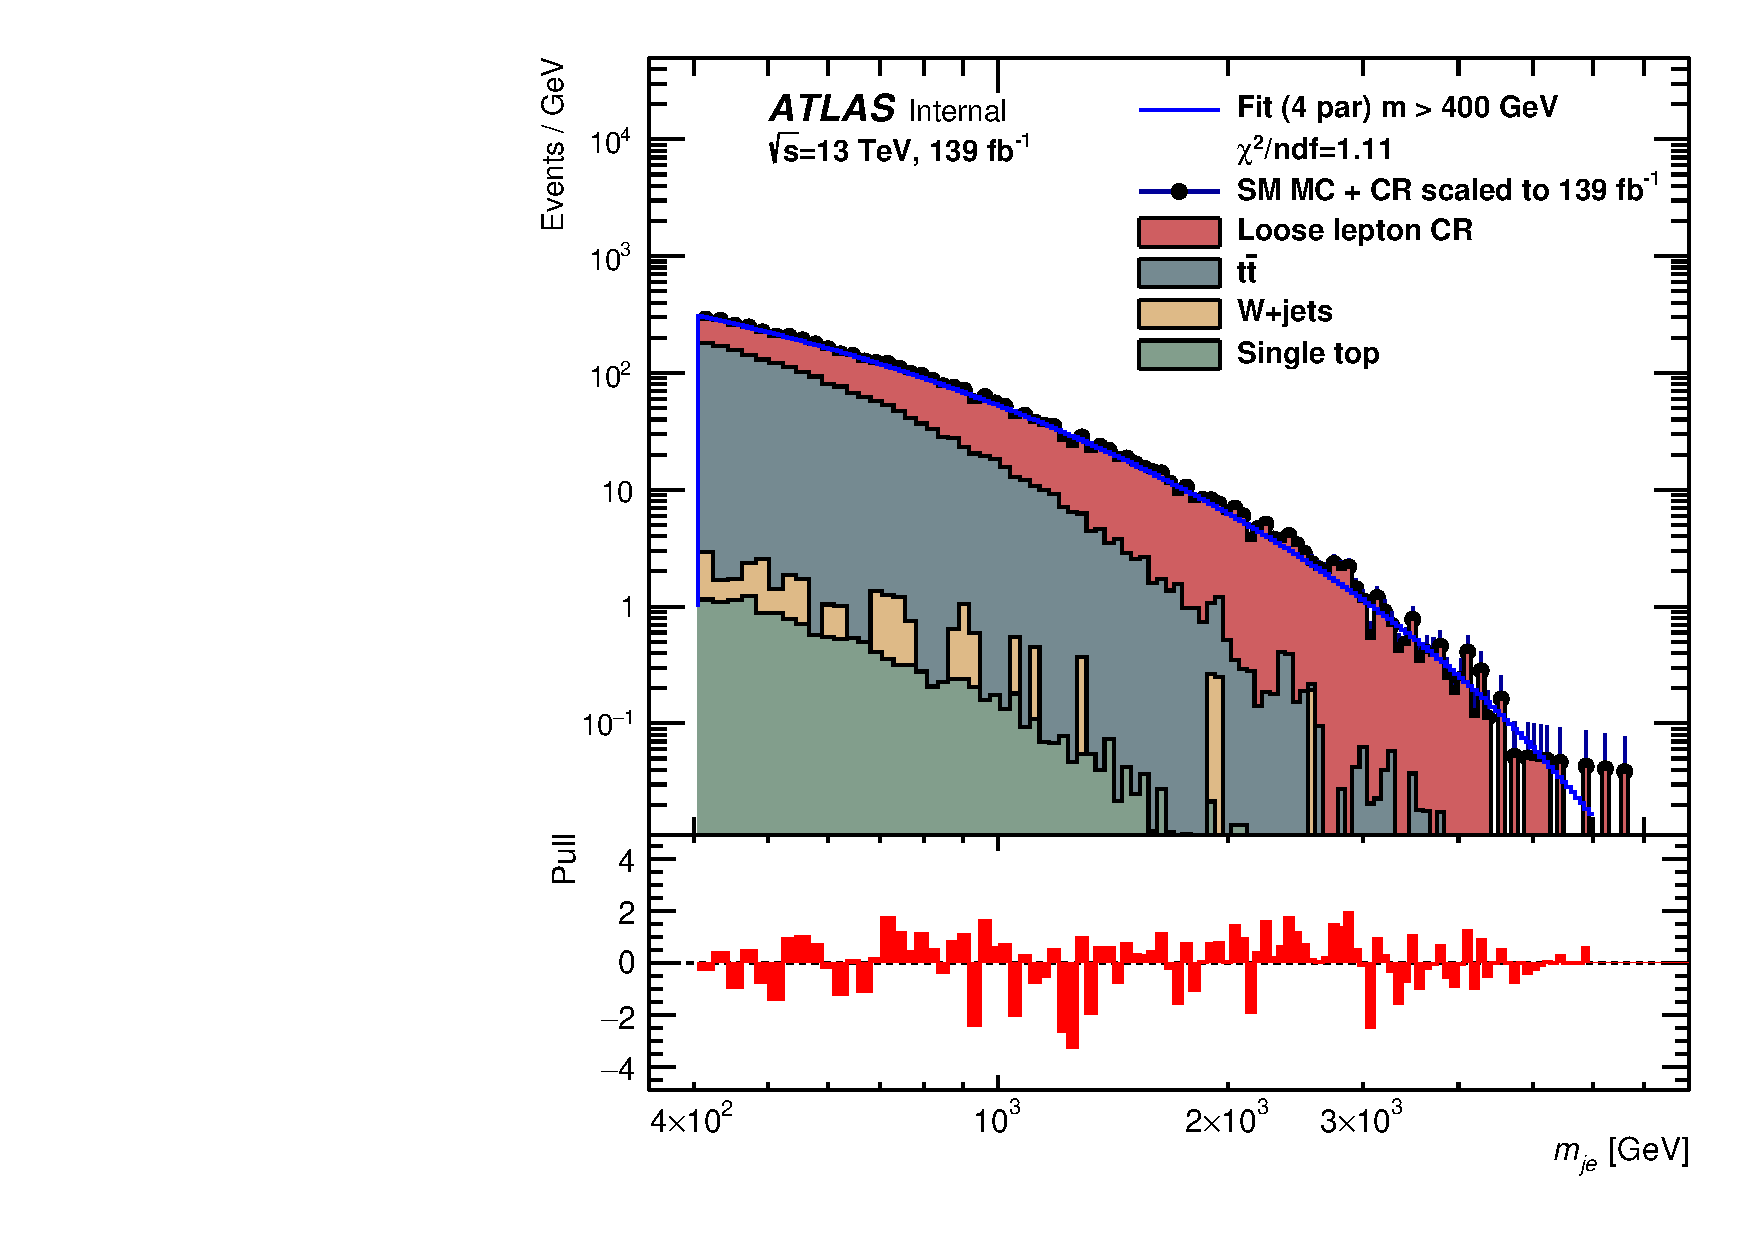
\includegraphics[scale=0.3]{figs/ch6/fit/variable_nosmooth/p4/1PB/output_SMMCplusCR_Mje_p4.pdf}%
    \caption{\mje \ using MC+LE-CR, p4}
    \end{subfigure}
    \hfill
    \begin{subfigure}[h]{0.4\linewidth}
    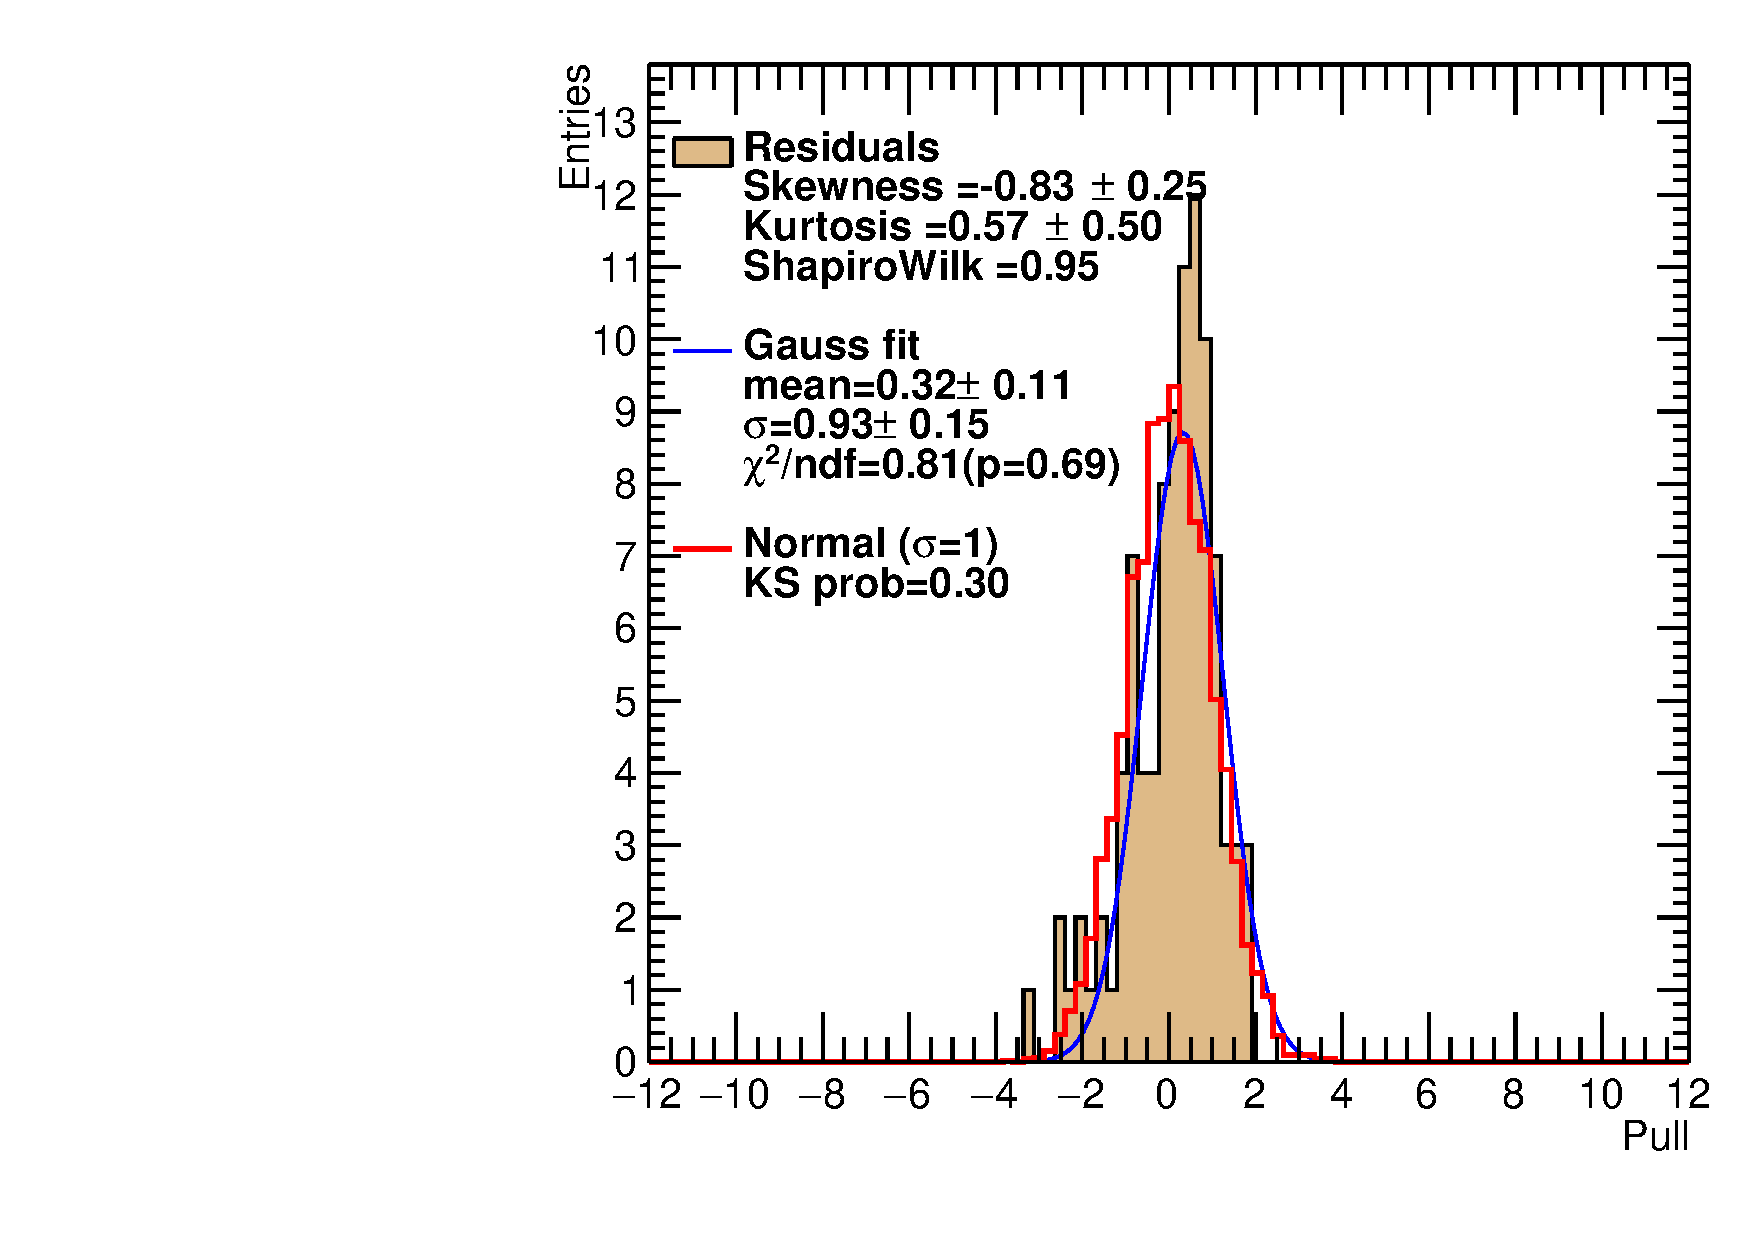
\includegraphics[scale=0.32]{figs/ch6/fit/variable_nosmooth/p4/1PB/pull_SMMCplusCR_Mje_p4.pdf}%
    \caption{pulls of \mje \ in p4}
    \end{subfigure}
    \hfill
    \begin{subfigure}[h]{0.38\linewidth}
    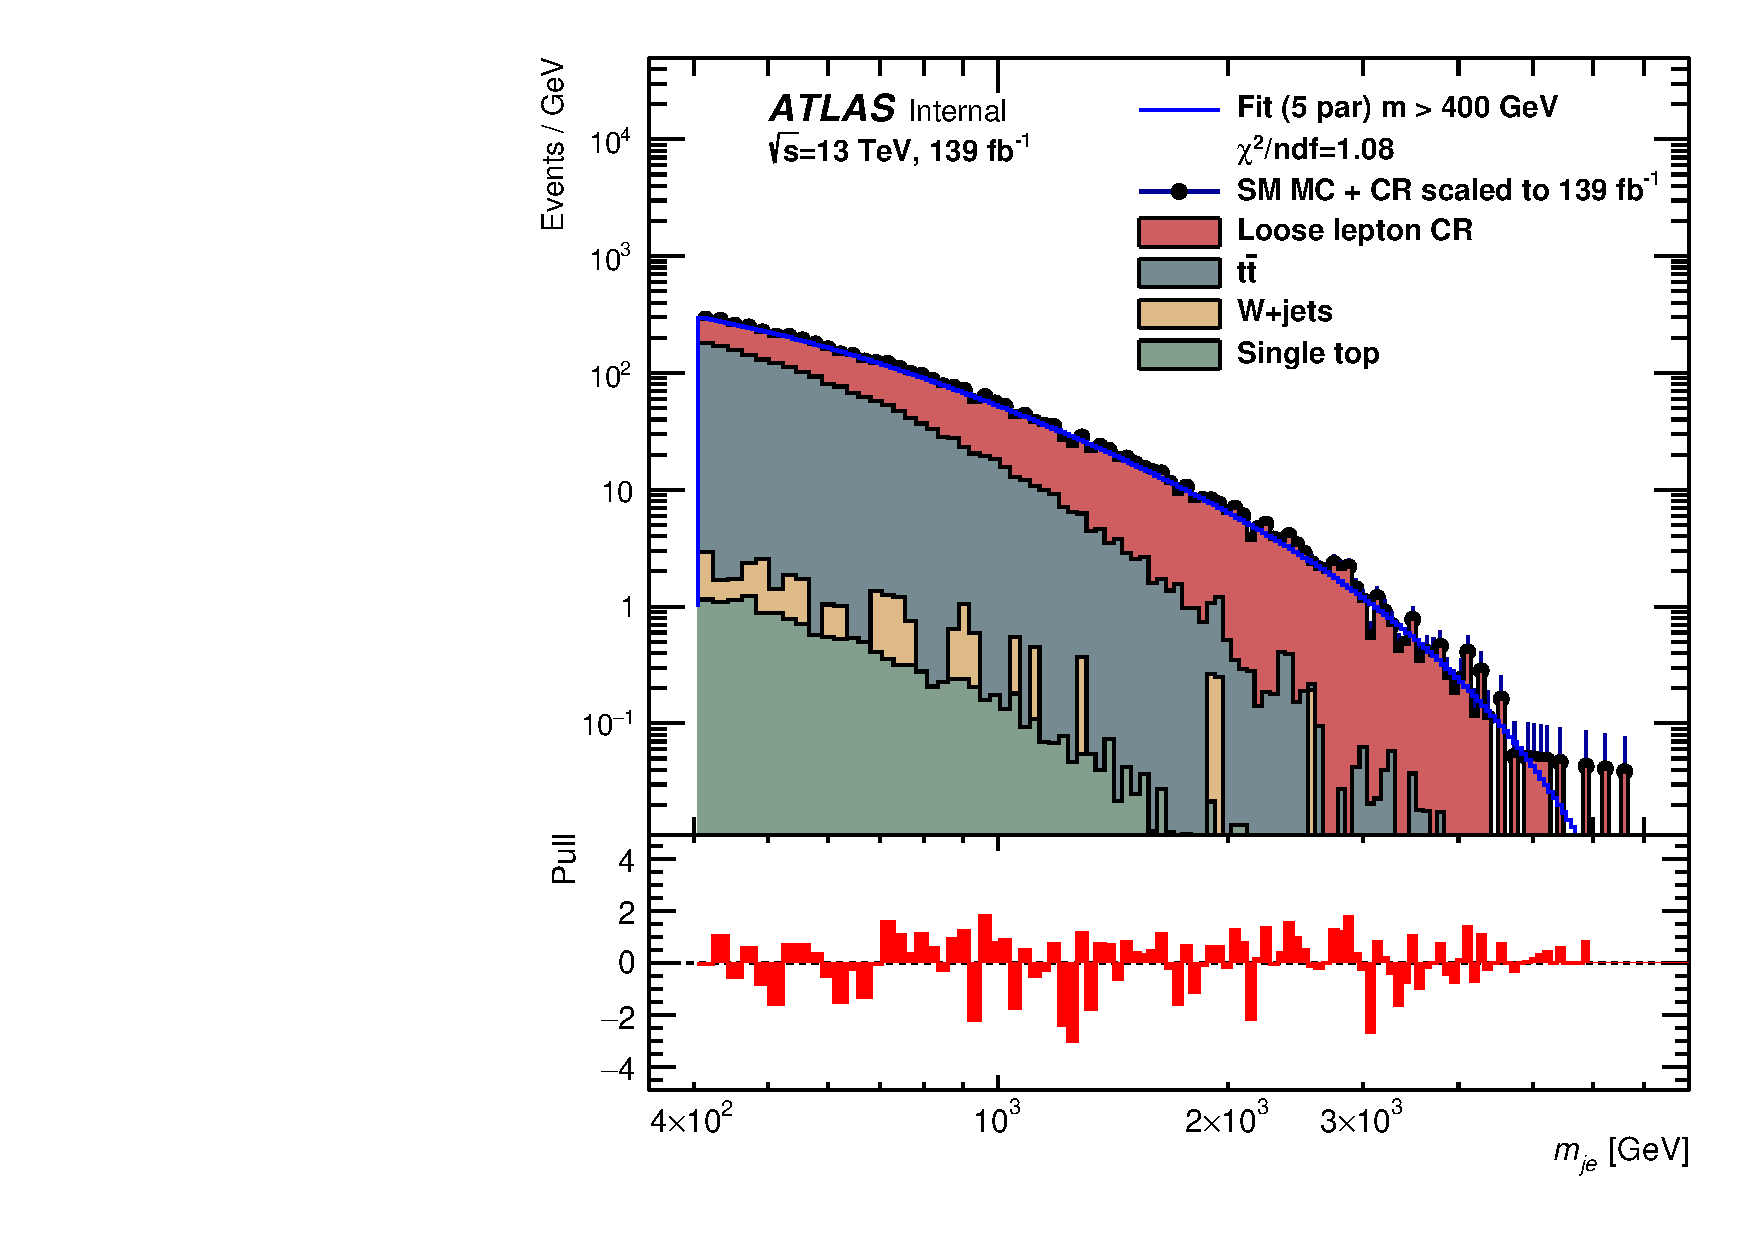
\includegraphics[scale=0.3]{figs/ch6/fit/variable_nosmooth/p5/1PB/output_SMMCplusCR_Mje_p5.pdf}%
     \caption{\mje \ using MC+LE-CR, p5}
     \end{subfigure}
     \hfill
    \begin{subfigure}[h]{0.4\linewidth}
    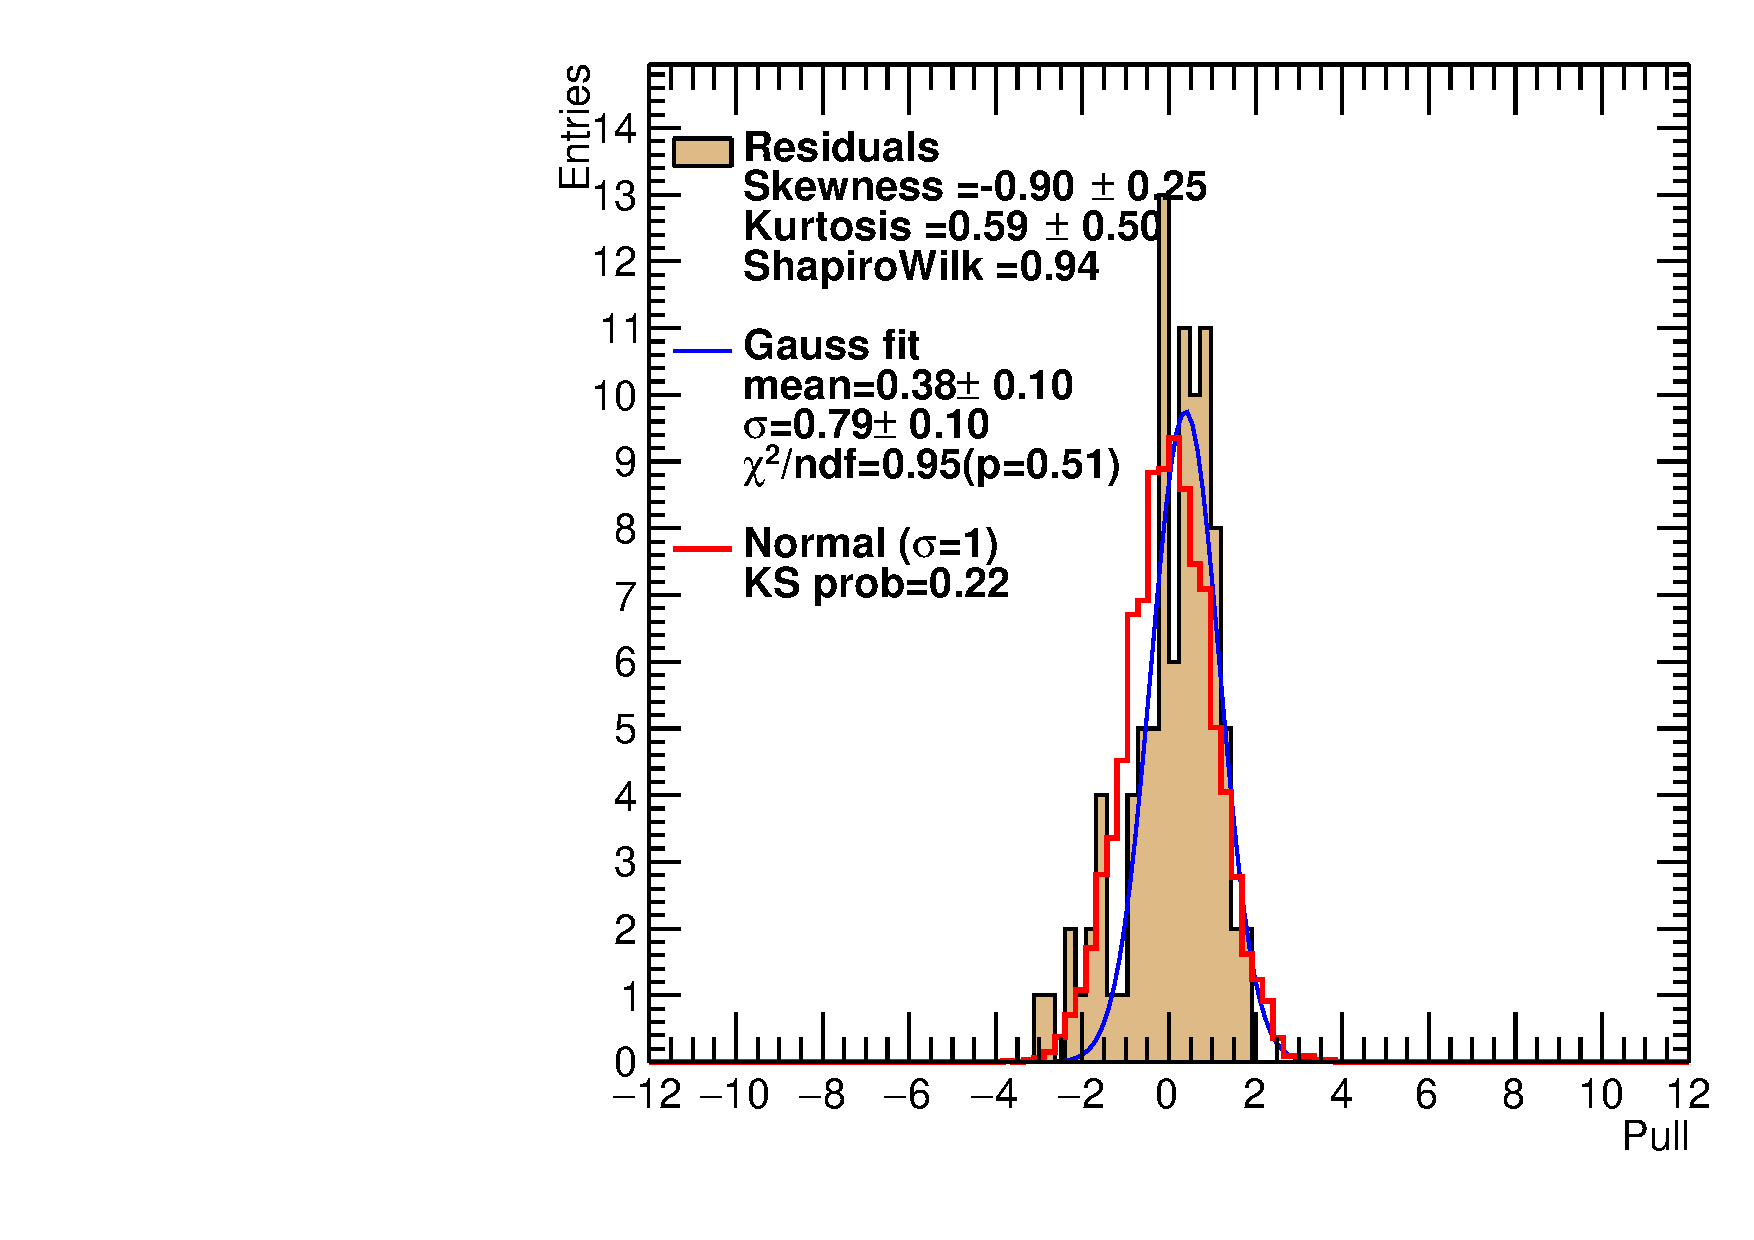
\includegraphics[scale=0.32]{figs/ch6/fit/variable_nosmooth/p5/1PB/pull_SMMCplusCR_Mje_p5.pdf}%
    \caption{pulls of \mje \ in p5}
    \end{subfigure}
    \caption{The \mje \ invariant masses with the p4 and p5 fit functions in the BSM region after the 1 pb AR cut is applied. The MC processes are scaled to their cross sections, while the LE-CR is used to fill the missing event rate. Pulls shown on the right.}
\label{fig:mje-fit-pulls-1pb}
\end{figure}

\newpage

\begin{figure}[ht]
    \centering
    \begin{subfigure}[h]{0.38\linewidth}
    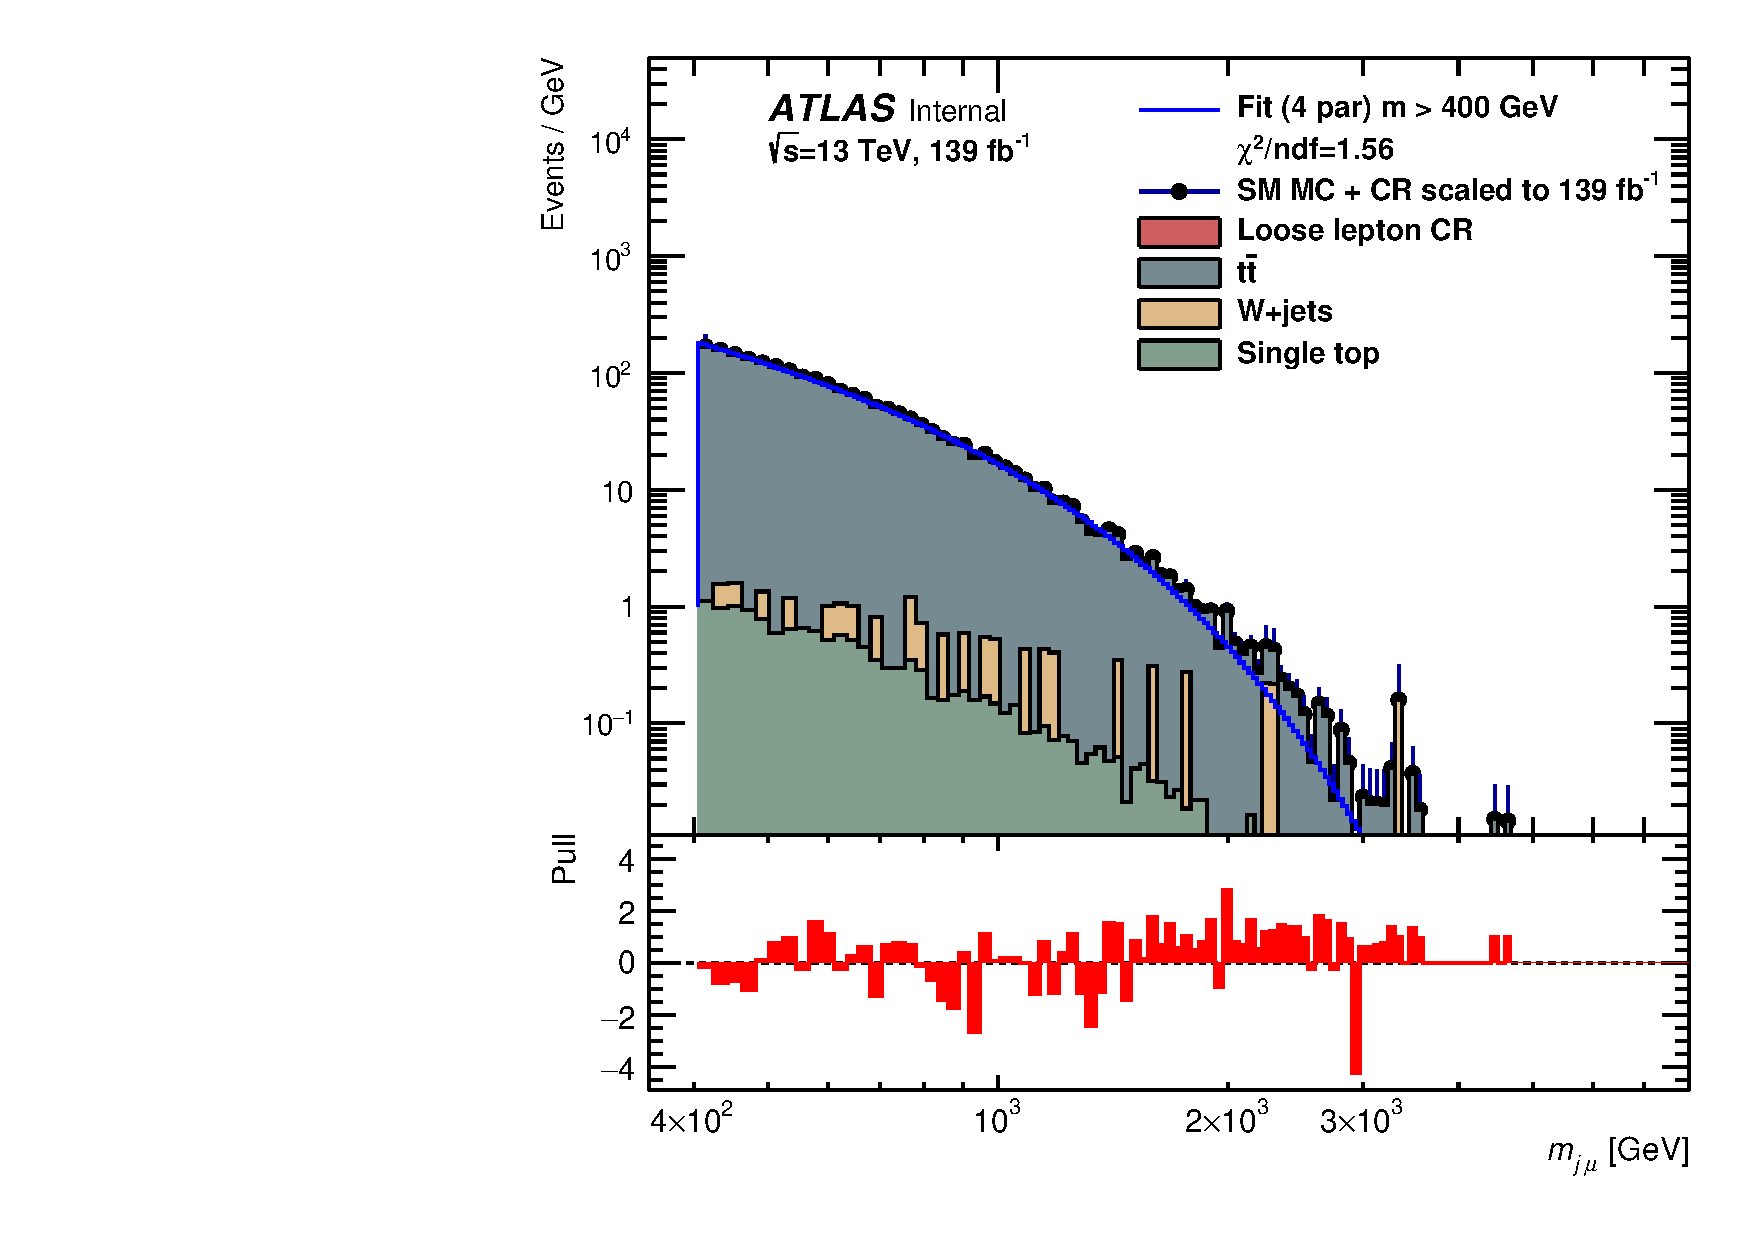
\includegraphics[scale=0.3]{figs/ch6/fit/variable_nosmooth/p4/1PB/output_SMMCplusCR_Mjm_p4.pdf}%
    \caption{\mjmu \ using MC+LE-CR, p4}
    \end{subfigure}
    \hfill
    \begin{subfigure}[h]{0.4\linewidth}
    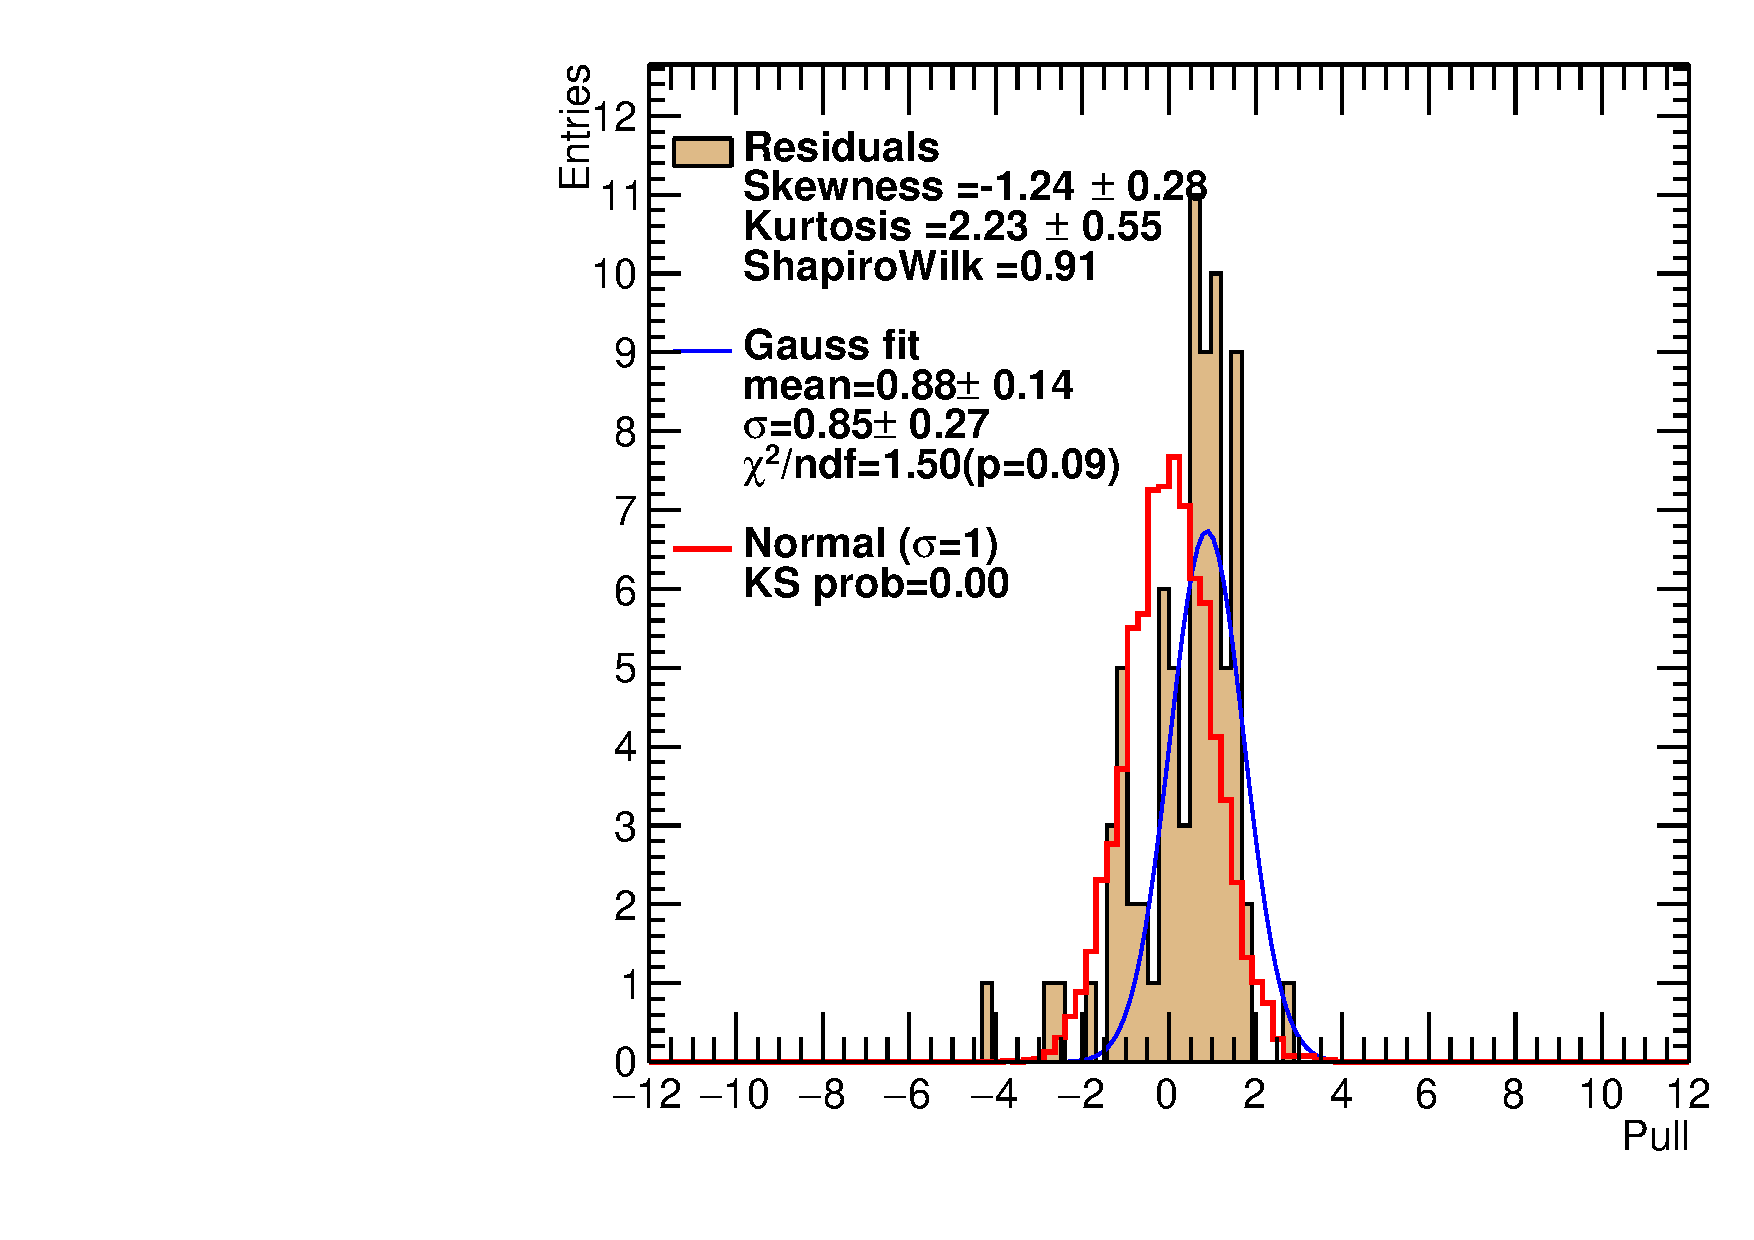
\includegraphics[scale=0.32]{figs/ch6/fit/variable_nosmooth/p4/1PB/pull_SMMCplusCR_Mjm_p4.pdf}%
    \caption{pulls of \mjmu \ in p4}
    \end{subfigure}
    \hfill
    \begin{subfigure}[h]{0.38\linewidth}
    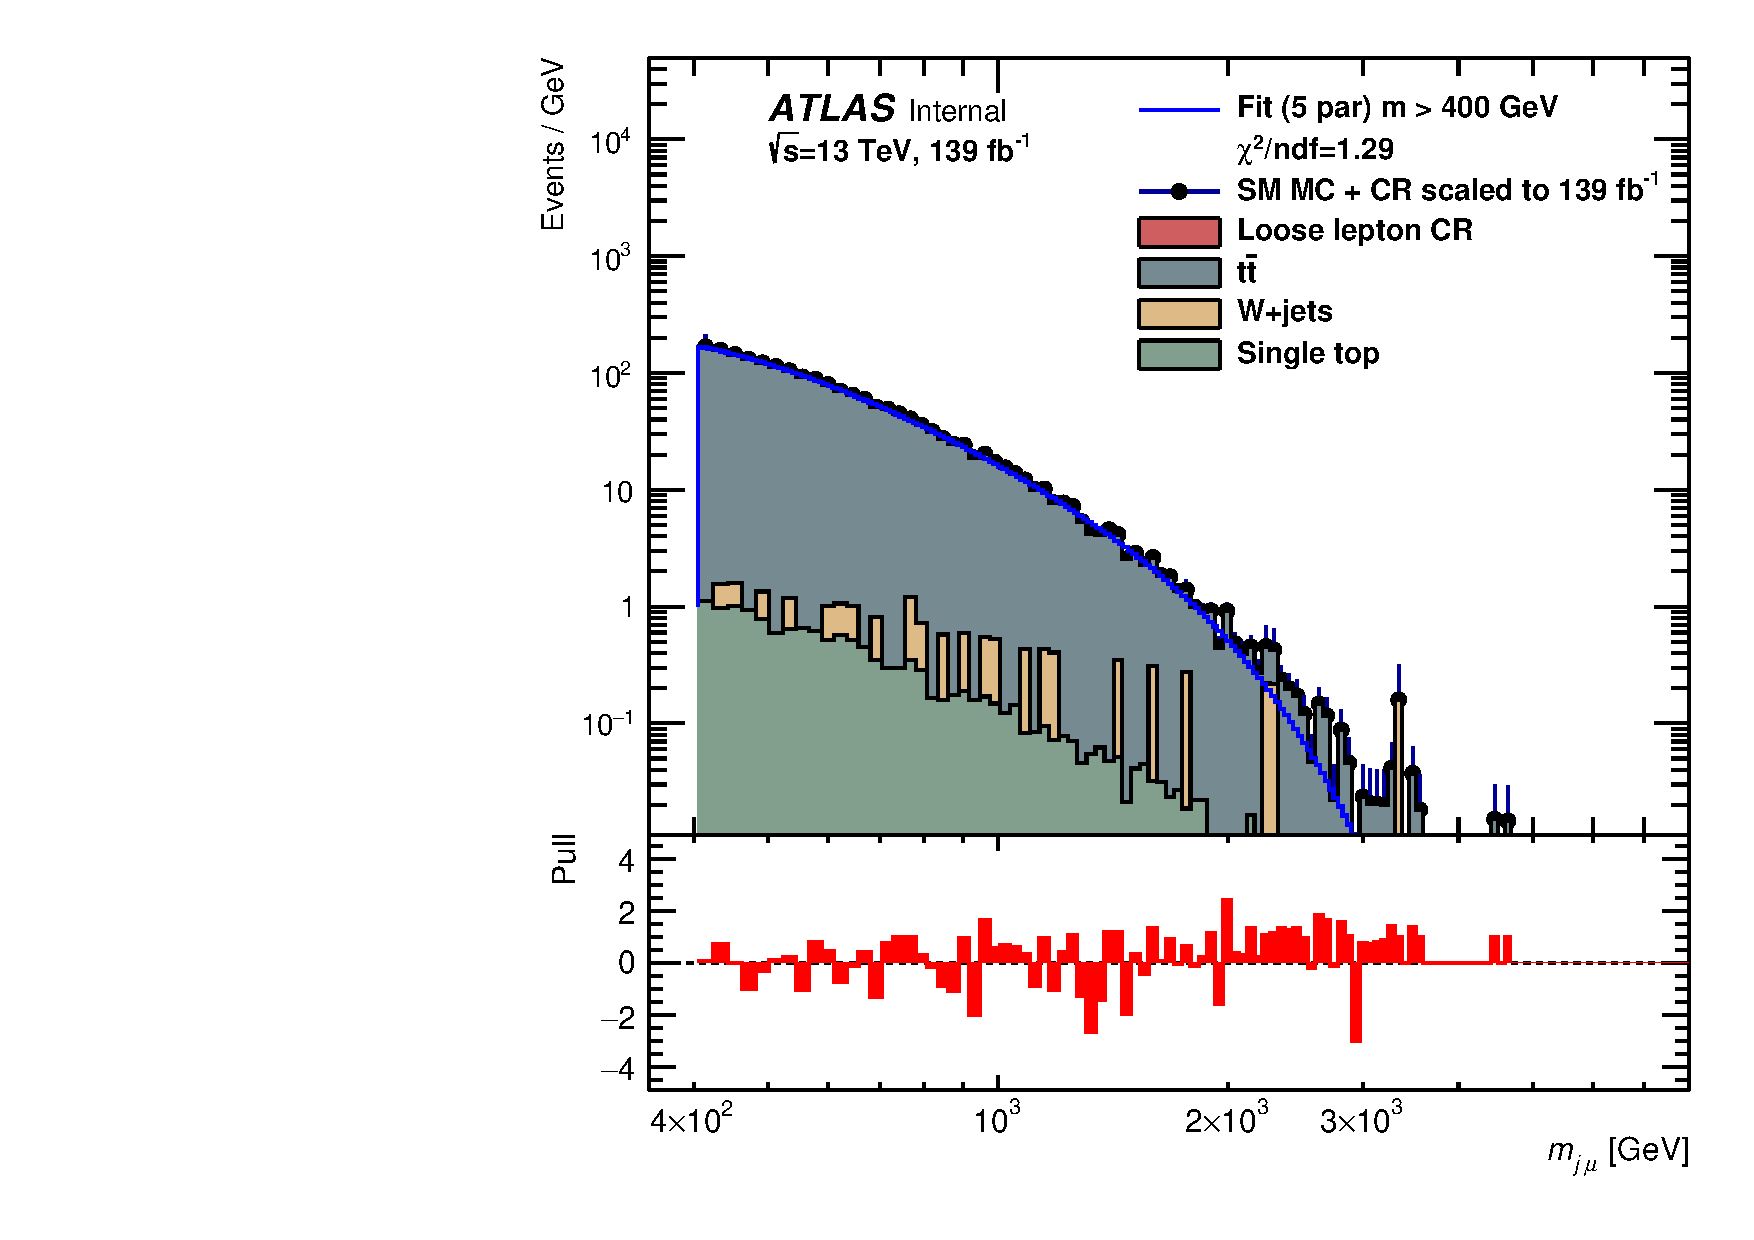
\includegraphics[scale=0.3]{figs/ch6/fit/variable_nosmooth/p5/1PB/output_SMMCplusCR_Mjm_p5.pdf}%
     \caption{\mjmu \ using MC+LE-CR, p5}
     \end{subfigure}
     \hfill
    \begin{subfigure}[h]{0.4\linewidth}
    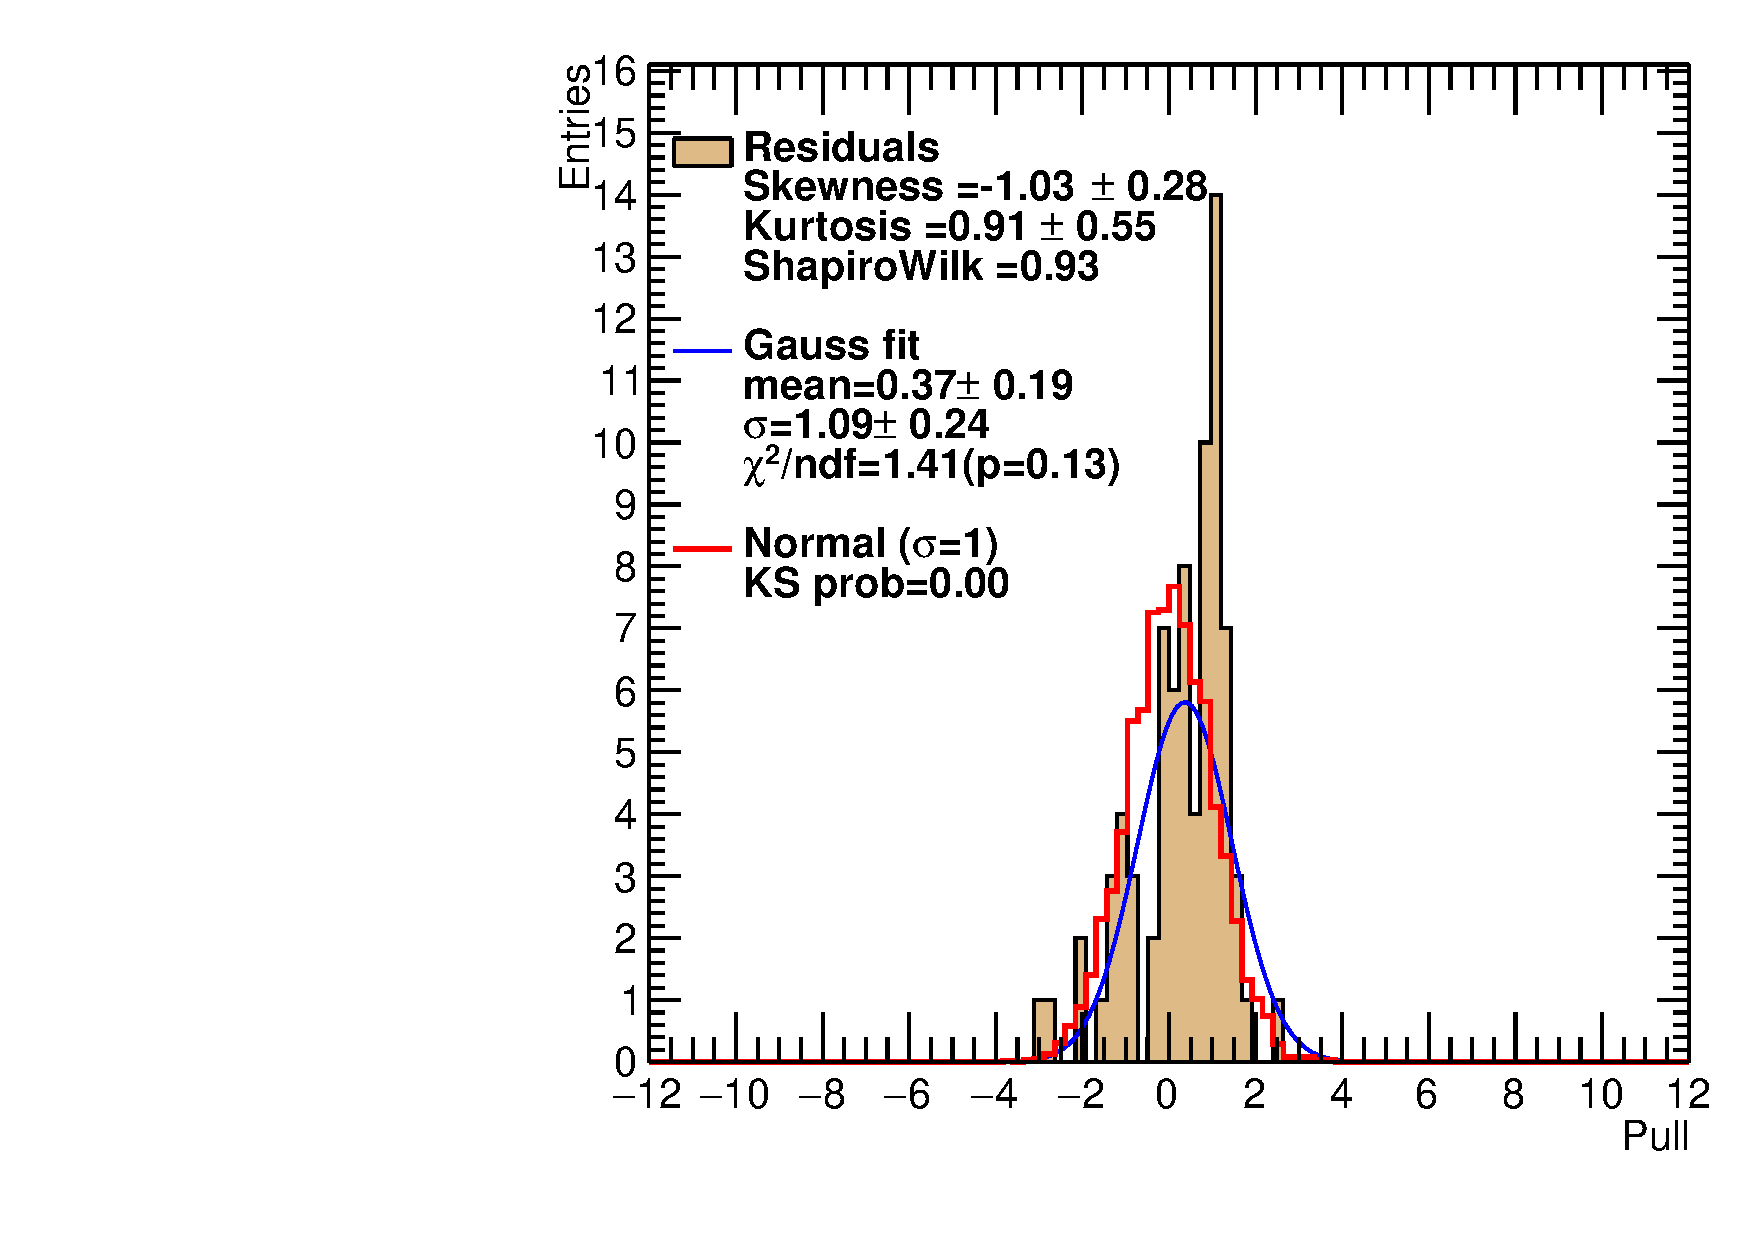
\includegraphics[scale=0.32]{figs/ch6/fit/variable_nosmooth/p5/1PB/pull_SMMCplusCR_Mjm_p5.pdf}%
    \caption{pulls of \mjmu \ in p5}
    \end{subfigure}
    \caption{The \mjmu \ invariant masses with the p4 and p5 fit functions in the BSM region after the 1 pb AR cut is applied. The MC processes are scaled to their cross sections, while the LE-CR is used to fill the missing event rate. Pulls shown on the right.}
\label{fig:mjm-fit-pulls-1pb}
\end{figure}

\newpage

\begin{figure}[ht]
    \centering
    \begin{subfigure}[h]{0.38\linewidth}
    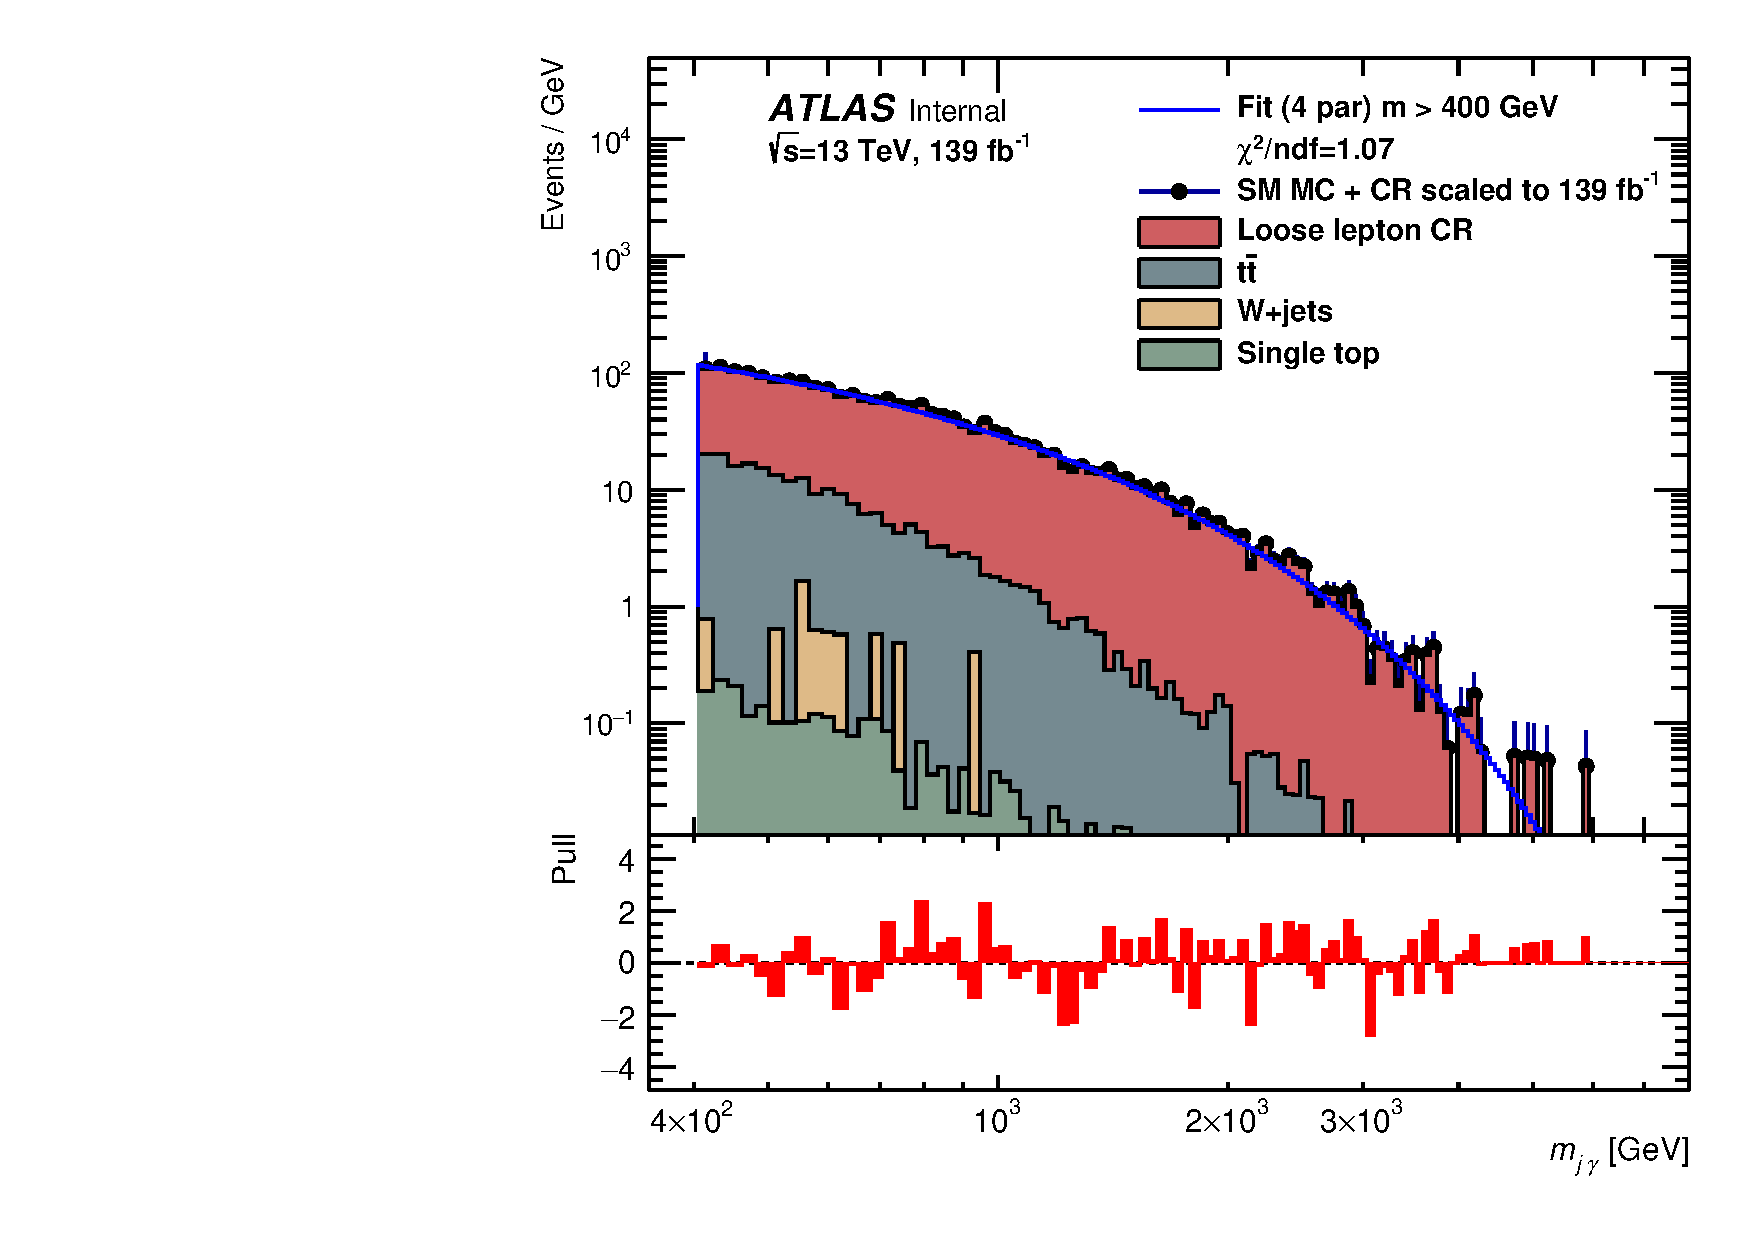
\includegraphics[scale=0.3]{figs/ch6/fit/variable_nosmooth/p4/1PB/output_SMMCplusCR_Mjg_p4.pdf}%
    \caption{\mjph \ using MC+LE-CR, p4}
    \end{subfigure}
    \hfill
    \begin{subfigure}[h]{0.4\linewidth}
    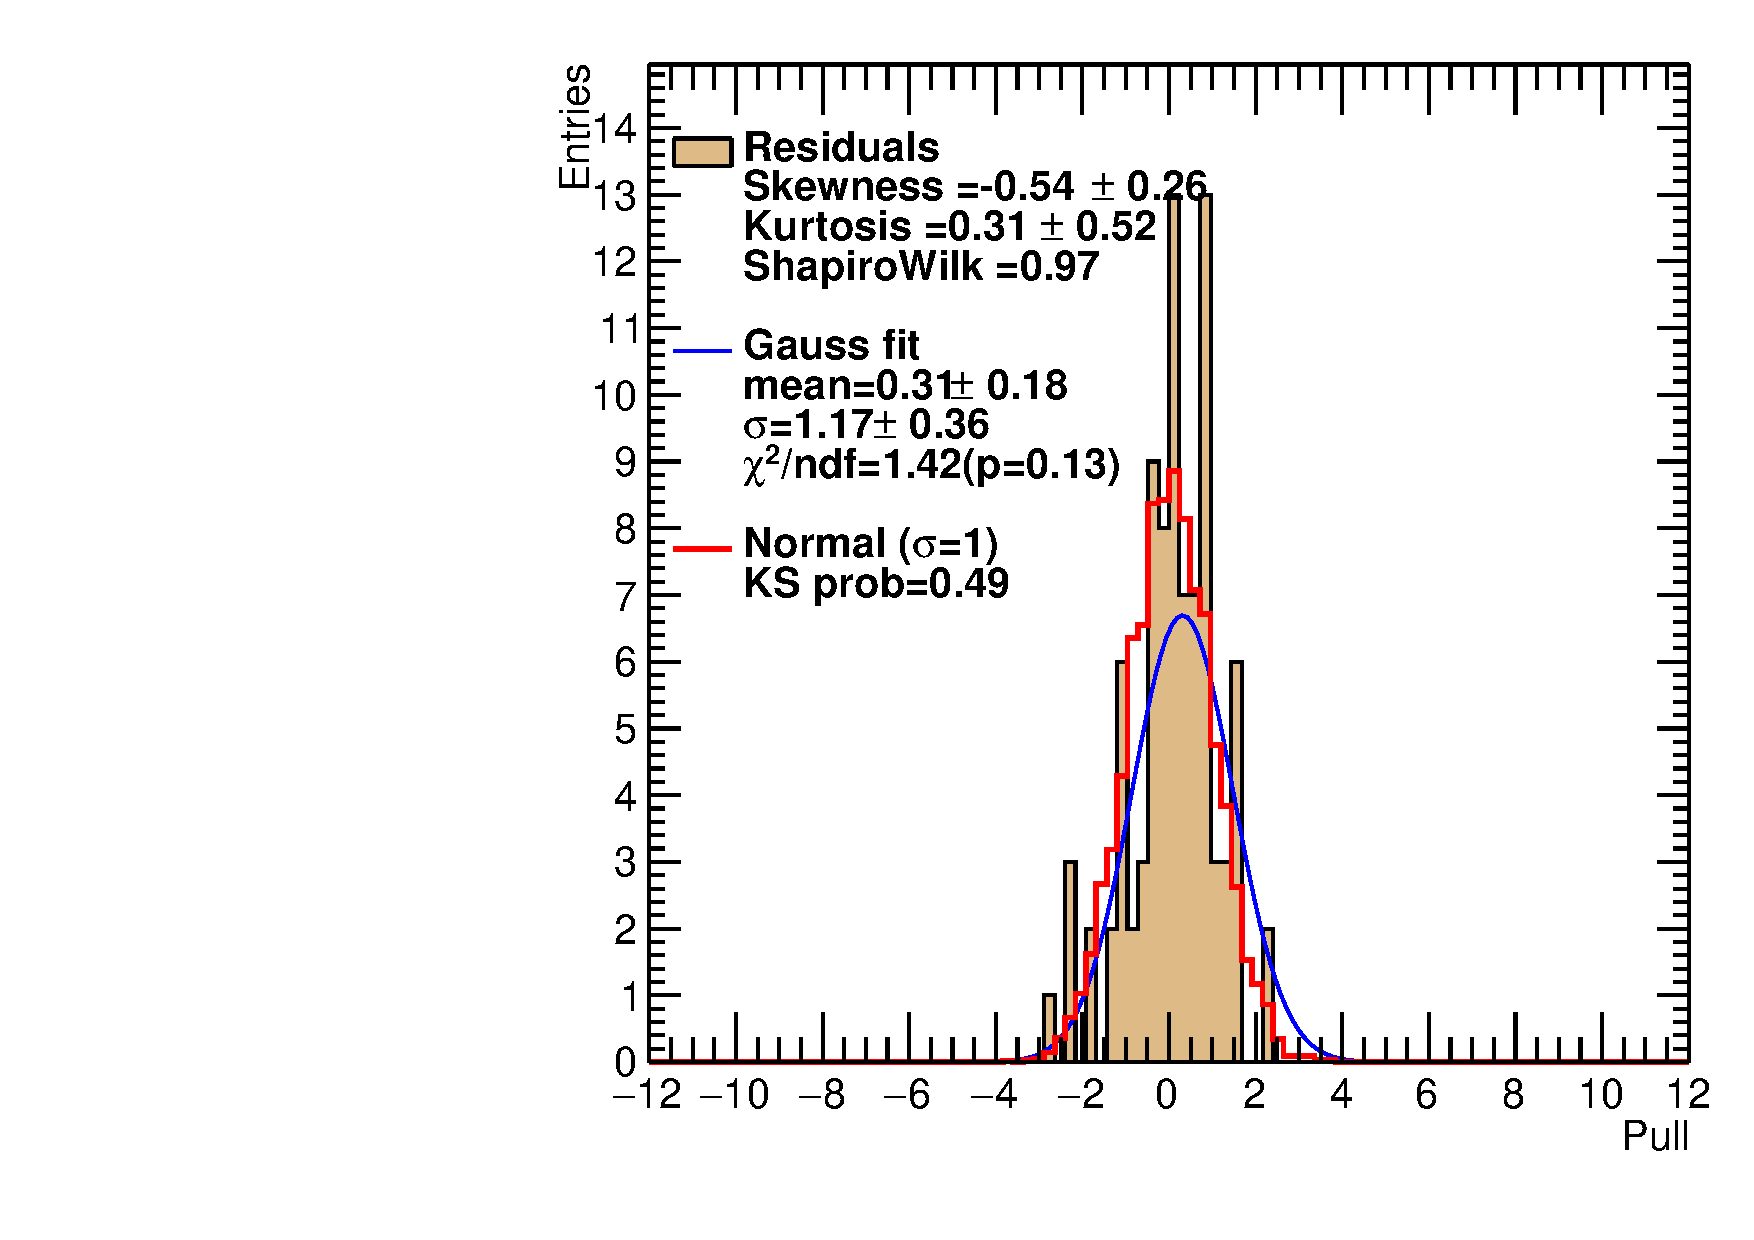
\includegraphics[scale=0.32]{figs/ch6/fit/variable_nosmooth/p4/1PB/pull_SMMCplusCR_Mjg_p4.pdf}%
    \caption{pulls of \mjph \ in p4}
    \end{subfigure}
    \hfill
    \begin{subfigure}[h]{0.38\linewidth}
    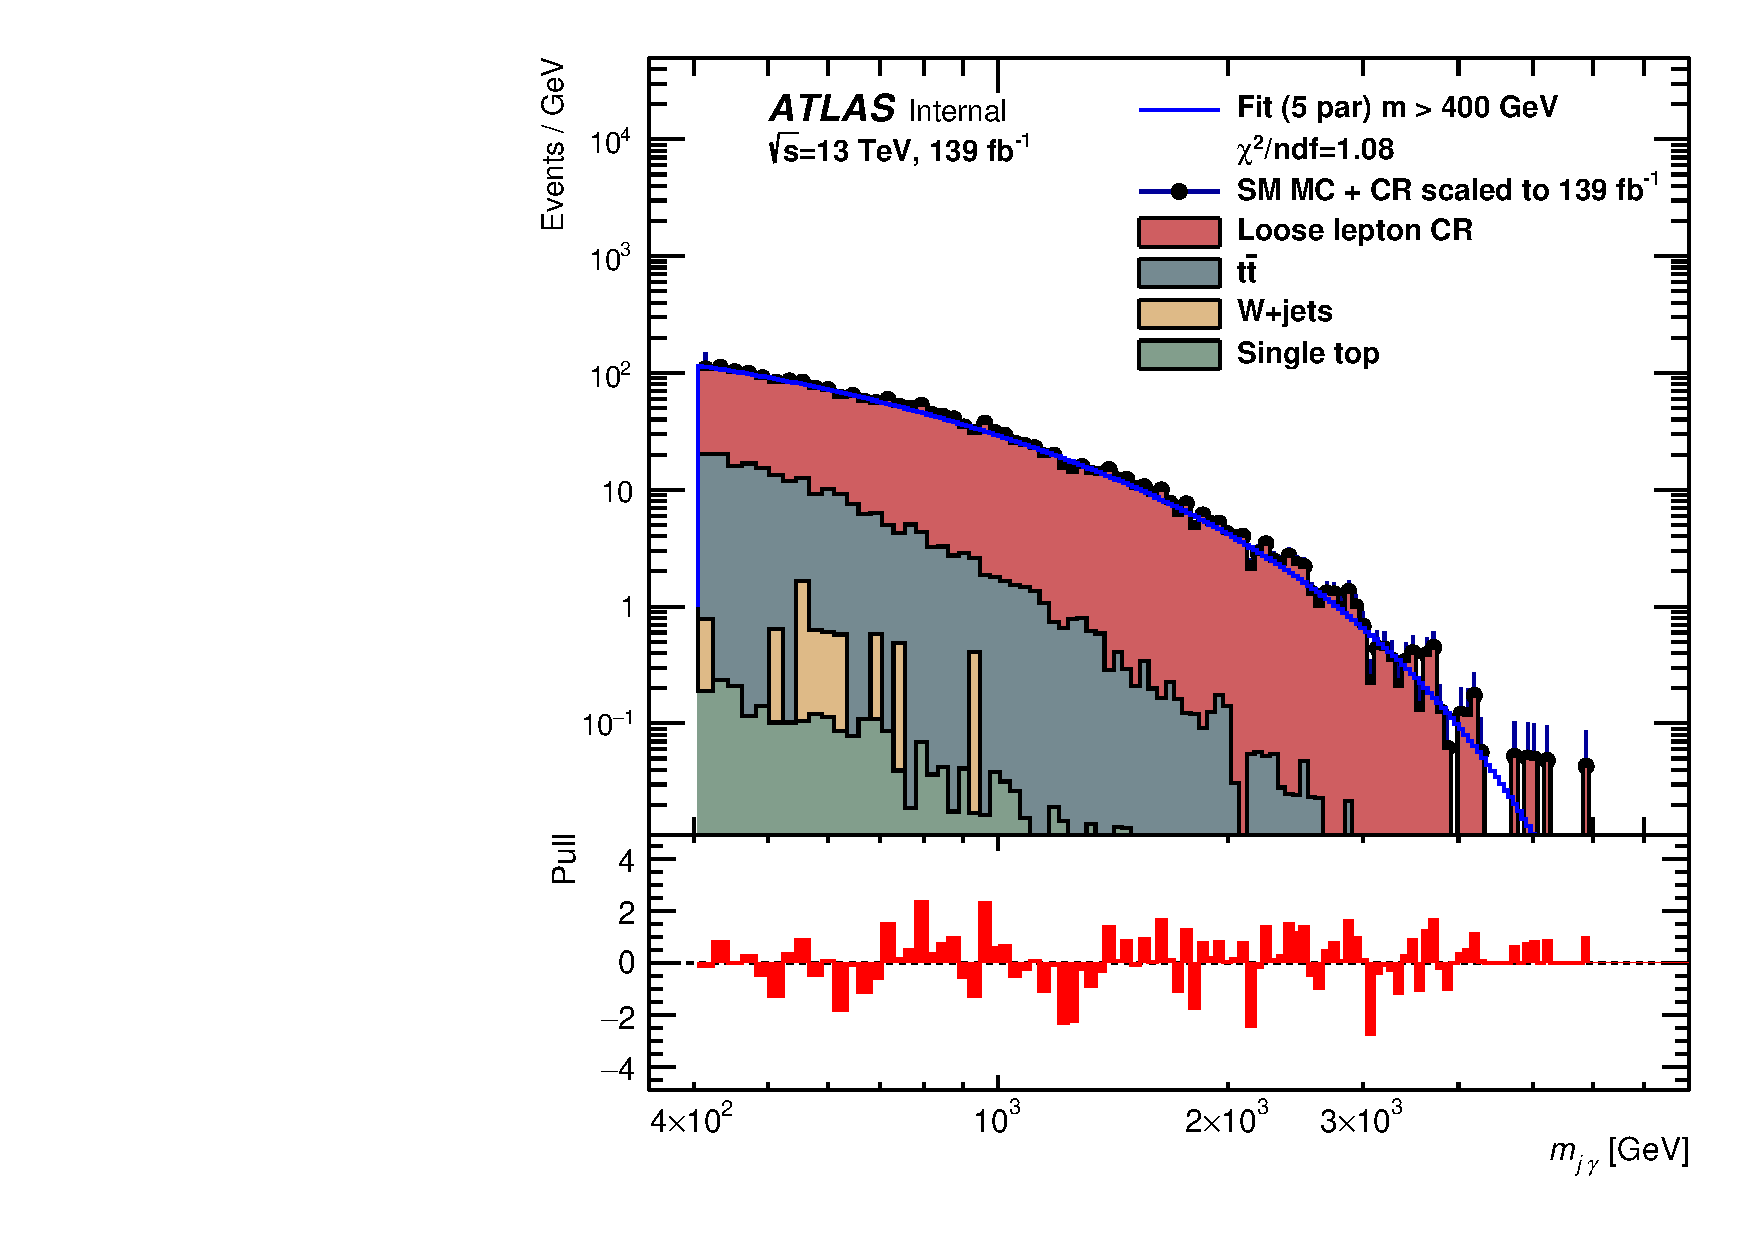
\includegraphics[scale=0.3]{figs/ch6/fit/variable_nosmooth/p5/1PB/output_SMMCplusCR_Mjg_p5.pdf}%
     \caption{\mjph \ using MC+LE-CR, p5}
     \end{subfigure}
     \hfill
    \begin{subfigure}[h]{0.4\linewidth}
    \includegraphics[scale=0.32]{figs/ch6/fit/variable_nosmooth/p5/1PB/pull_SMMCplusCR_Mjg_p5.pdf}%
    \caption{pulls of \mjph \ in p5}
    \end{subfigure}
    \caption{The \mjph \ invariant masses with the p4 and p5 fit functions in the BSM region after the 1 pb AR cut is applied. The MC processes are scaled to their cross sections, while the LE-CR is used to fill the missing event rate. Pulls shown on the right.}
\label{fig:mjg-fit-pulls-1pb}
\end{figure}

\newpage

\begin{figure}[ht]
    \centering
    \begin{subfigure}[h]{0.38\linewidth}
    \includegraphics[scale=0.3]{figs/ch6/fit/variable_nosmooth/p4/1PB/output_SMMCplusCR_Mbe_p4.pdf}%
    \caption{\mbe \ using MC+LE-CR, p4}
    \end{subfigure}
    \hfill
    \begin{subfigure}[h]{0.4\linewidth}
    \includegraphics[scale=0.32]{figs/ch6/fit/variable_nosmooth/p4/1PB/pull_SMMCplusCR_Mbe_p4.pdf}%
    \caption{pulls of \mbe \ in p4}
    \end{subfigure}
    \hfill
    \begin{subfigure}[h]{0.38\linewidth}
    \includegraphics[scale=0.3]{figs/ch6/fit/variable_nosmooth/p5/1PB/output_SMMCplusCR_Mbe_p5.pdf}%
     \caption{\mbe \ using MC+LE-CR, p5}
     \end{subfigure}
     \hfill
    \begin{subfigure}[h]{0.4\linewidth}
    \includegraphics[scale=0.32]{figs/ch6/fit/variable_nosmooth/p5/1PB/pull_SMMCplusCR_Mbe_p5.pdf}%
    \caption{pulls of \mbe \ in p5}
    \end{subfigure}
    \caption{The \mbe \ invariant masses with the p4 and p5 fit functions in the BSM region after the 1 pb AR cut is applied. The MC processes are scaled to their cross sections, while the LE-CR is used to fill the missing event rate. Pulls shown on the right.}
\label{fig:mbe-fit-pulls-1pb}
\end{figure}

\newpage

\begin{figure}[ht]
    \centering
    \begin{subfigure}[h]{0.38\linewidth}
    \includegraphics[scale=0.3]{figs/ch6/fit/variable_nosmooth/p4/1PB/output_SMMCplusCR_Mbm_p4.pdf}%
    \caption{\mbmu \ using MC+LE-CR, p4}
    \end{subfigure}
    \hfill
    \begin{subfigure}[h]{0.4\linewidth}
    \includegraphics[scale=0.32]{figs/ch6/fit/variable_nosmooth/p4/1PB/pull_SMMCplusCR_Mbm_p4.pdf}%
    \caption{pulls of \mbmu \ in p4}
    \end{subfigure}
    \hfill
    \begin{subfigure}[h]{0.38\linewidth}
    \includegraphics[scale=0.3]{figs/ch6/fit/variable_nosmooth/p5/1PB/output_SMMCplusCR_Mbm_p5.pdf}%
     \caption{\mbmu \ using MC+LE-CR, p5}
     \end{subfigure}
     \hfill
    \begin{subfigure}[h]{0.4\linewidth}
    \includegraphics[scale=0.32]{figs/ch6/fit/variable_nosmooth/p5/1PB/pull_SMMCplusCR_Mbm_p5.pdf}%
    \caption{pulls of \mbmu \ in p5}
    \end{subfigure}
    \caption{The \mbmu \ invariant masses with the p4 and p5 fit functions in the BSM region after the 1 pb AR cut is applied. The MC processes are scaled to their cross sections, while the LE-CR is used to fill the missing event rate. Pulls shown on the right.}
\label{fig:mbm-fit-pulls-1pb}
\end{figure}

\newpage

\begin{figure}[ht]
    \centering
    \begin{subfigure}[h]{0.38\linewidth}
    \includegraphics[scale=0.3]{figs/ch6/fit/variable_nosmooth/p4/1PB/output_SMMCplusCR_Mbg_p4.pdf}%
    \caption{\mbph \ using MC+LE-CR, p4}
    \end{subfigure}
    \hfill
    \begin{subfigure}[h]{0.4\linewidth}
    \includegraphics[scale=0.32]{figs/ch6/fit/variable_nosmooth/p4/1PB/pull_SMMCplusCR_Mbg_p4.pdf}%
    \caption{pulls of \mbph \ in p4}
    \end{subfigure}
    \hfill
    \begin{subfigure}[h]{0.38\linewidth}
    \includegraphics[scale=0.3]{figs/ch6/fit/variable_nosmooth/p5/1PB/output_SMMCplusCR_Mbg_p5.pdf}%
     \caption{\mjph \ using MC+LE-CR, p5}
     \end{subfigure}
     \hfill
    \begin{subfigure}[h]{0.4\linewidth}
    \includegraphics[scale=0.32]{figs/ch6/fit/variable_nosmooth/p5/1PB/pull_SMMCplusCR_Mbg_p5.pdf}%
    \caption{pulls of \mbph \ in p5}
    \end{subfigure}
    \caption{The \mbph \ invariant masses with the p4 and p5 fit functions in the BSM region after the 1 pb AR cut is applied. The MC processes are scaled to their cross sections, while the LE-CR is used to fill the missing event rate. Pulls shown on the right.}
\label{fig:mbg-fit-pulls-1pb}
\end{figure}

\newpage

\vspace*{0.5in}

\section{Statistical Fit Function Studies for 0.1pb AR}
\label{appendix:01pb-fit-studies}
%\addcontentsline{toc}{chapter}{Statistical Fit Function Studies for 0.1pb AR}
\numberwithin{equation}{chapter}
\setcounter{equation}{0}

Just as in Appendix~\ref{appendix:1pb-fit-studies}, only the p4 and p5 fit functions are studied. The results can be seen in Table X and the figures show the MC+LE-CR along with 
their pulls. This region only has 14K events, therefore finding a reasonable fit function was inconclusive, just as in the 1 pb \gls{ar}.

\begin{multicols}{3}
    \begin{itemize}
    \item Figure~\ref{fig:mjj-fit-pulls-01pb} 0.1pb \mjj
    \item Figure~\ref{fig:mjb-fit-pulls-01pb} 0.1pb \mjb
    \item Figure~\ref{fig:mbb-fit-pulls-01pb} 0.1pb \mbb
    \item Figure~\ref{fig:mje-fit-pulls-01pb} 0.1pb \mje
    \item Figure~\ref{fig:mjm-fit-pulls-01pb} 0.1pb \mjmu
    \item Figure~\ref{fig:mjg-fit-pulls-01pb} 0.1pb \mjph
    \item Figure~\ref{fig:mbe-fit-pulls-01pb} 0.1pb \mbe
    \item Figure~\ref{fig:mjm-fit-pulls-01pb} 0.1pb \mbmu
    \item Figure~\ref{fig:mbg-fit-pulls-01pb} 0.1pb \mbph
    \end{itemize}
 \end{multicols}

 \newpage

 
\begin{table}[!htbp]
   \begin{center}
      \begin{scriptsize}
      \begin{tabular}{|c|c|c|c|c|c|c|c|c|c|c|c|}
         \hline
         {Mass} & {region} & {p} & {Fit $\chi^2$} & {Pull $\mu$} & {$\Delta\mu$} & {$\sigma$} & {$\Delta\sigma$} & {Gaus $\chi^2$} & {KS} & {Shapiro}  \\
         \hline
         \mjj & 0.1 pb & 4 & 1.066981 & 0.439052 & 0.154240 & 1.066725 & 0.168530 & 0.520639 & 0.114105 & 0.982610 \\
         \mjb & 0.1 pb & 4 & 1.030326 & 0.478555 & 0.107806 & 0.706963 & 0.108466 & 1.092364 & 0.054007 & 0.913377 \\
         \mbb & 0.1 pb & 4 & 1.104344 & 0.476400 & 0.405565 & 1.478379 & 0.507329 & 0.607558 & 0.104235 & 0.967501 \\
         \mje & 0.1 pb & 4 & 0.988952 & 0.527118 & 0.087665 & 0.647729 & 0.091518 & 0.773745 & 0.008889 & 0.934337 \\
         \mjmu & 0.1 pb & 4 & 1.247852 & 0.688118 & 0.120311 & 0.710719 & 0.131556 & 0.958169 & 0.012524 & 0.894489 \\
         \mjph & 0.1 pb & 4 & 0.766672 & 0.325899 & 0.104514 & 0.712873 & 0.103878 & 0.994939 & 0.093205 & 0.958485 \\
         \mbe & 0.1 pb & 4 & 0.689806 & 0.222383 & 0.179162 & 0.911493 & 0.183285 & 0.341040 & 0.355303 & 0.965579 \\
         \mbmu & 0.1 pb & 4 & 0.994301 & 0.577633 & 1.529995 & 2.193773 & 1.597088 & 1.426726 & 0.091036 & 0.934948 \\
         \mbph & 0.1 pb & 4 & 0.532739 & 0.123343 & 0.153080 & 0.761905 & 0.157570 & 0.373211 & 0.509120 & 0.982694 \\
         \hline
         \mjj & 0.1 pb & 5 & 0.982026 & 0.323078 & 0.147239 & 1.053884 & 0.137738 & 0.611454 & 0.178563 & 0.984839 \\
         \mjb & 0.1 pb & 5 & 1.032755 & 0.424803 & 0.110022 & 0.755037 & 0.111329 & 0.853758 & 0.046379 & 0.911716 \\
         \mbb & 0.1 pb & 5 & 1.115241 & 0.510098 & 0.184014 & 1.048742 & 0.241893 & 0.562814 & 0.337324 & 0.970615 \\
         \mje & 0.1 pb & 5 & 0.996203 & 0.232937 & 0.133625 & 0.900851 & 0.117146 & 1.034730 & 0.002092 & 0.934982 \\
         \mjmu & 0.1 pb & 5 & 1.150431 & 0.443298 & 0.176520 & 0.758198 & 0.239118 & 0.846013 & 0.017779 & 0.889262 \\
         \mjph & 0.1 pb & 5 & 0.764039 & 0.158883 & 0.118088 & 0.817065 & 0.101391 & 0.592739 & 0.412045 & 0.969030 \\
         \mbe & 0.1 pb & 5 & 0.708264 & 0.186595 & 0.214779 & 0.993727 & 0.222814 & 0.713869 & 0.355303 & 0.965863 \\
         \mbmu & 0.1 pb & 5 & 0.985081 & 0.139081 & 0.285717 & 1.249059 & 0.346504 & 0.645550 & 0.723507 & 0.950681 \\
         \mbph & 0.1 pb & 5 & 0.619378 & 0.147059 & 0.163189 & 0.805034 & 0.202471 & 0.437407 & 0.329640 & 0.988531 \\
         \hline
      \end{tabular}
   \end{scriptsize}
   \end{center}
   \caption{Statistical quantities for SM MC+LE-CR fit for the 1 pb AR.}
   \label{tab:stat-quantities-01PB-SMMCplusCR}
\end{table}


 \newpage

 \begin{figure}[ht]
    \centering
    \begin{subfigure}[h]{0.38\linewidth}
    \includegraphics[scale=0.3]{figs/ch6/fit/variable_nosmooth/p4/01PB/output_SMMCplusCR_Mjj_p4.pdf}%
    \caption{\mjj \ using MC+LE-CR, p4}
    \end{subfigure}
    \hfill
    \begin{subfigure}[h]{0.4\linewidth}
    \includegraphics[scale=0.32]{figs/ch6/fit/variable_nosmooth/p4/01PB/pull_SMMCplusCR_Mjj_p4.pdf}%
    \caption{pulls of \mjj \ in p4}
    \end{subfigure}
    \hfill
    \begin{subfigure}[h]{0.38\linewidth}
    \includegraphics[scale=0.3]{figs/ch6/fit/variable_nosmooth/p5/01PB/output_SMMCplusCR_Mjj_p5.pdf}%
     \caption{\mjj \ using MC+LE-CR, p5}
     \end{subfigure}
     \hfill
    \begin{subfigure}[h]{0.4\linewidth}
    \includegraphics[scale=0.32]{figs/ch6/fit/variable_nosmooth/p5/01PB/pull_SMMCplusCR_Mjj_p5.pdf}%
    \caption{pulls of \mjj \ in p5}
    \end{subfigure}
    \caption{The \mjj \ invariant masses with the p4 and p5 fit functions in the BSM region after the 0.1 pb AR cut is applied. The MC processes are scaled to their cross sections, while the LE-CR is used to fill the missing event rate. Pulls shown on the right.}
\label{fig:mjj-fit-pulls-01pb}
\end{figure}

\newpage

\begin{figure}[ht]
    \centering
    \begin{subfigure}[h]{0.38\linewidth}
    \includegraphics[scale=0.3]{figs/ch6/fit/variable_nosmooth/p4/01PB/output_SMMCplusCR_Mjb_p4.pdf}%
    \caption{\mjb \ using MC+LE-CR, p4}
    \end{subfigure}
    \hfill
    \begin{subfigure}[h]{0.4\linewidth}
    \includegraphics[scale=0.32]{figs/ch6/fit/variable_nosmooth/p4/01PB/pull_SMMCplusCR_Mjb_p4.pdf}%
    \caption{pulls of \mjb \ in p4}
    \end{subfigure}
    \hfill
    \begin{subfigure}[h]{0.38\linewidth}
    \includegraphics[scale=0.3]{figs/ch6/fit/variable_nosmooth/p5/01PB/output_SMMCplusCR_Mjb_p5.pdf}%
     \caption{\mjb \ using MC+LE-CR, p5}
     \end{subfigure}
     \hfill
    \begin{subfigure}[h]{0.4\linewidth}
    \includegraphics[scale=0.32]{figs/ch6/fit/variable_nosmooth/p5/01PB/pull_SMMCplusCR_Mjb_p5.pdf}%
    \caption{pulls of \mjb \ in p5}
    \end{subfigure}
    \caption{The \mjb \ invariant masses with the p4 and p5 fit functions in the BSM region after the 0.1 pb AR cut is applied. The MC processes are scaled to their cross sections, while the LE-CR is used to fill the missing event rate. Pulls shown on the right.}
\label{fig:mjb-fit-pulls-01pb}
\end{figure}

\newpage

\begin{figure}[ht]
    \centering
    \begin{subfigure}[h]{0.38\linewidth}
    \includegraphics[scale=0.3]{figs/ch6/fit/variable_nosmooth/p4/01PB/output_SMMCplusCR_Mbb_p4.pdf}%
    \caption{\mbb \ using MC+LE-CR, p4}
    \end{subfigure}
    \hfill
    \begin{subfigure}[h]{0.4\linewidth}
    \includegraphics[scale=0.32]{figs/ch6/fit/variable_nosmooth/p4/01PB/pull_SMMCplusCR_Mbb_p4.pdf}%
    \caption{pulls of \mbb \ in p4}
    \end{subfigure}
    \hfill
    \begin{subfigure}[h]{0.38\linewidth}
    \includegraphics[scale=0.3]{figs/ch6/fit/variable_nosmooth/p5/01PB/output_SMMCplusCR_Mbb_p5.pdf}%
     \caption{\mbb \ using MC+LE-CR, p5}
     \end{subfigure}
     \hfill
    \begin{subfigure}[h]{0.4\linewidth}
    \includegraphics[scale=0.32]{figs/ch6/fit/variable_nosmooth/p5/01PB/pull_SMMCplusCR_Mbb_p5.pdf}%
    \caption{pulls of \mbb \ in p5}
    \end{subfigure}
    \caption{The \mbb \ invariant masses with the p4 and p5 fit functions in the BSM region after the 0.1 pb AR cut is applied. The MC processes are scaled to their cross sections, while the LE-CR is used to fill the missing event rate. Pulls shown on the right.}
\label{fig:mbb-fit-pulls-01pb}
\end{figure}

\newpage

\begin{figure}[ht]
    \centering
    \begin{subfigure}[h]{0.38\linewidth}
    \includegraphics[scale=0.3]{figs/ch6/fit/variable_nosmooth/p4/01PB/output_SMMCplusCR_Mje_p4.pdf}%
    \caption{\mje \ using MC+LE-CR, p4}
    \end{subfigure}
    \hfill
    \begin{subfigure}[h]{0.4\linewidth}
    \includegraphics[scale=0.32]{figs/ch6/fit/variable_nosmooth/p4/01PB/pull_SMMCplusCR_Mje_p4.pdf}%
    \caption{pulls of \mje \ in p4}
    \end{subfigure}
    \hfill
    \begin{subfigure}[h]{0.38\linewidth}
    \includegraphics[scale=0.3]{figs/ch6/fit/variable_nosmooth/p5/01PB/output_SMMCplusCR_Mje_p5.pdf}%
     \caption{\mje \ using MC+LE-CR, p5}
     \end{subfigure}
     \hfill
    \begin{subfigure}[h]{0.4\linewidth}
    \includegraphics[scale=0.32]{figs/ch6/fit/variable_nosmooth/p5/01PB/pull_SMMCplusCR_Mje_p5.pdf}%
    \caption{pulls of \mje \ in p5}
    \end{subfigure}
    \caption{The \mje \ invariant masses with the p4 and p5 fit functions in the BSM region after the 0.1 pb AR cut is applied. The MC processes are scaled to their cross sections, while the LE-CR is used to fill the missing event rate. Pulls shown on the right.}
\label{fig:mje-fit-pulls-01pb}
\end{figure}

\newpage

\begin{figure}[ht]
    \centering
    \begin{subfigure}[h]{0.38\linewidth}
    \includegraphics[scale=0.3]{figs/ch6/fit/variable_nosmooth/p4/01PB/output_SMMCplusCR_Mjm_p4.pdf}%
    \caption{\mjmu \ using MC+LE-CR, p4}
    \end{subfigure}
    \hfill
    \begin{subfigure}[h]{0.4\linewidth}
    \includegraphics[scale=0.32]{figs/ch6/fit/variable_nosmooth/p4/01PB/pull_SMMCplusCR_Mjm_p4.pdf}%
    \caption{pulls of \mjmu \ in p4}
    \end{subfigure}
    \hfill
    \begin{subfigure}[h]{0.38\linewidth}
    \includegraphics[scale=0.3]{figs/ch6/fit/variable_nosmooth/p5/01PB/output_SMMCplusCR_Mjm_p5.pdf}%
     \caption{\mjmu \ using MC+LE-CR, p5}
     \end{subfigure}
     \hfill
    \begin{subfigure}[h]{0.4\linewidth}
    \includegraphics[scale=0.32]{figs/ch6/fit/variable_nosmooth/p5/01PB/pull_SMMCplusCR_Mjm_p5.pdf}%
    \caption{pulls of \mjmu \ in p5}
    \end{subfigure}
    \caption{The \mjmu \ invariant masses with the p4 and p5 fit functions in the BSM region after the 0.1 pb AR cut is applied. The MC processes are scaled to their cross sections, while the LE-CR is used to fill the missing event rate. Pulls shown on the right.}
\label{fig:mjm-fit-pulls-01pb}
\end{figure}

\newpage

\begin{figure}[ht]
    \centering
    \begin{subfigure}[h]{0.38\linewidth}
    \includegraphics[scale=0.3]{figs/ch6/fit/variable_nosmooth/p4/01PB/output_SMMCplusCR_Mjg_p4.pdf}%
    \caption{\mjph \ using MC+LE-CR, p4}
    \end{subfigure}
    \hfill
    \begin{subfigure}[h]{0.4\linewidth}
    \includegraphics[scale=0.32]{figs/ch6/fit/variable_nosmooth/p4/01PB/pull_SMMCplusCR_Mjg_p4.pdf}%
    \caption{pulls of \mjph \ in p4}
    \end{subfigure}
    \hfill
    \begin{subfigure}[h]{0.38\linewidth}
    \includegraphics[scale=0.3]{figs/ch6/fit/variable_nosmooth/p5/01PB/output_SMMCplusCR_Mjg_p5.pdf}%
     \caption{\mjph \ using MC+LE-CR, p5}
     \end{subfigure}
     \hfill
    \begin{subfigure}[h]{0.4\linewidth}
    \includegraphics[scale=0.32]{figs/ch6/fit/variable_nosmooth/p5/01PB/pull_SMMCplusCR_Mjg_p5.pdf}%
    \caption{pulls of \mjph \ in p5}
    \end{subfigure}
    \caption{The \mjph \ invariant masses with the p4 and p5 fit functions in the BSM region after the 0.1 pb AR cut is applied. The MC processes are scaled to their cross sections, while the LE-CR is used to fill the missing event rate. Pulls shown on the right.}
\label{fig:mjg-fit-pulls-01pb}
\end{figure}

\newpage

\begin{figure}[ht]
    \centering
    \begin{subfigure}[h]{0.38\linewidth}
    \includegraphics[scale=0.3]{figs/ch6/fit/variable_nosmooth/p4/01PB/output_SMMCplusCR_Mbe_p4.pdf}%
    \caption{\mbe \ using MC+LE-CR, p4}
    \end{subfigure}
    \hfill
    \begin{subfigure}[h]{0.4\linewidth}
    \includegraphics[scale=0.32]{figs/ch6/fit/variable_nosmooth/p4/01PB/pull_SMMCplusCR_Mbe_p4.pdf}%
    \caption{pulls of \mbe \ in p4}
    \end{subfigure}
    \hfill
    \begin{subfigure}[h]{0.38\linewidth}
    \includegraphics[scale=0.3]{figs/ch6/fit/variable_nosmooth/p5/01PB/output_SMMCplusCR_Mbe_p5.pdf}%
     \caption{\mbe \ using MC+LE-CR, p5}
     \end{subfigure}
     \hfill
    \begin{subfigure}[h]{0.4\linewidth}
    \includegraphics[scale=0.32]{figs/ch6/fit/variable_nosmooth/p5/01PB/pull_SMMCplusCR_Mbe_p5.pdf}%
    \caption{pulls of \mbe \ in p5}
    \end{subfigure}
    \caption{The \mbe \ invariant masses with the p4 and p5 fit functions in the BSM region after the 0.1 pb AR cut is applied. The MC processes are scaled to their cross sections, while the LE-CR is used to fill the missing event rate. Pulls shown on the right.}
\label{fig:mbe-fit-pulls-01pb}
\end{figure}

\newpage

\begin{figure}[ht]
    \centering
    \begin{subfigure}[h]{0.38\linewidth}
    \includegraphics[scale=0.3]{figs/ch6/fit/variable_nosmooth/p4/01PB/output_SMMCplusCR_Mbm_p4.pdf}%
    \caption{\mbmu \ using MC+LE-CR, p4}
    \end{subfigure}
    \hfill
    \begin{subfigure}[h]{0.4\linewidth}
    \includegraphics[scale=0.32]{figs/ch6/fit/variable_nosmooth/p4/01PB/pull_SMMCplusCR_Mbm_p4.pdf}%
    \caption{pulls of \mbmu \ in p4}
    \end{subfigure}
    \hfill
    \begin{subfigure}[h]{0.38\linewidth}
    \includegraphics[scale=0.3]{figs/ch6/fit/variable_nosmooth/p5/01PB/output_SMMCplusCR_Mbm_p5.pdf}%
     \caption{\mbmu \ using MC+LE-CR, p5}
     \end{subfigure}
     \hfill
    \begin{subfigure}[h]{0.4\linewidth}
    \includegraphics[scale=0.32]{figs/ch6/fit/variable_nosmooth/p5/01PB/pull_SMMCplusCR_Mbm_p5.pdf}%
    \caption{pulls of \mbmu \ in p5}
    \end{subfigure}
    \caption{The \mbmu \ invariant masses with the p4 and p5 fit functions in the BSM region after the 0.1 pb AR cut is applied. The MC processes are scaled to their cross sections, while the LE-CR is used to fill the missing event rate. Pulls shown on the right.}
\label{fig:mbm-fit-pulls-01pb}
\end{figure}

\newpage

\begin{figure}[ht]
    \centering
    \begin{subfigure}[h]{0.38\linewidth}
    \includegraphics[scale=0.3]{figs/ch6/fit/variable_nosmooth/p4/01PB/output_SMMCplusCR_Mbg_p4.pdf}%
    \caption{\mbph \ using MC+LE-CR, p4}
    \end{subfigure}
    \hfill
    \begin{subfigure}[h]{0.4\linewidth}
    \includegraphics[scale=0.32]{figs/ch6/fit/variable_nosmooth/p4/01PB/pull_SMMCplusCR_Mbg_p4.pdf}%
    \caption{pulls of \mbph \ in p4}
    \end{subfigure}
    \hfill
    \begin{subfigure}[h]{0.38\linewidth}
    \includegraphics[scale=0.3]{figs/ch6/fit/variable_nosmooth/p5/01PB/output_SMMCplusCR_Mbg_p5.pdf}%
     \caption{\mjph \ using MC+LE-CR, p5}
     \end{subfigure}
     \hfill
    \begin{subfigure}[h]{0.4\linewidth}
    \includegraphics[scale=0.32]{figs/ch6/fit/variable_nosmooth/p5/01PB/pull_SMMCplusCR_Mbg_p5.pdf}%
    \caption{pulls of \mbph \ in p5}
    \end{subfigure}
    \caption{The \mbph \ invariant masses with the p4 and p5 fit functions in the BSM region after the 0.1 pb AR cut is applied. The MC processes are scaled to their cross sections, while the LE-CR is used to fill the missing event rate. Pulls shown on the right.}
\label{fig:mbg-fit-pulls-01pb}
\end{figure}

\newpage

\vspace*{0.5in}

\section{Fit Studies on 10\% of Data}
\label{appendix:10data-fit-studies}
%\addcontentsline{toc}{chapter}{Fit Studies on 10\% of Data}
\numberwithin{equation}{chapter}
\setcounter{equation}{0}

The 5p fit function was shown to be the best choice from the three functions studied. However, there were few cases that strained the function and required a further step 
to ensure that this 5p fir function is indeed the proper choice. It was recommended to select randomly a 10\% data sample and scale it by 10 to reproduce a realisitc 
event rate while also smoothing the distribution. The Savitzky-Golay filter \cite{smoothing} was used for smoothing. Figures \ref{fig:10data-fit-pulls-jj}-\ref{fig:10data-fit-pulls-be} show the smoothed and extrapolated 10\% of real data. 
Good agreements with the 5p fit function is observed, confirming to biases in the masses after the 10 pb \gls{ar}. 

\newpage

\begin{figure}[H]
    \centering
    \begin{subfigure}[h]{0.38\linewidth}
    \includegraphics[scale=0.3]{figs/app/10data/pub_mass_10per_extrapolate_jj.pdf}%
    \caption{jj 10\% data, 5p fit }
    \end{subfigure}
    \hfill
    \begin{subfigure}[h]{0.4\linewidth}
    \includegraphics[scale=0.32]{figs/app/10data/pub_mass_10per_extrapolate_residuals_jj.pdf}%
    \caption{pulls of jj in 5p fit}
    \end{subfigure}
    \hfill
    \begin{subfigure}[h]{0.38\linewidth}
    \includegraphics[scale=0.3]{figs//app/10data/pub_mass_10per_extrapolate_jb.pdf}%
     \caption{jb 10\% of data, 5p fit}
     \end{subfigure}
     \hfill
    \begin{subfigure}[h]{0.4\linewidth}
    \includegraphics[scale=0.32]{figs/app/10data/pub_mass_10per_extrapolate_residuals_jb.pdf}%
    \caption{pulls of jb in 5p fit}
    \end{subfigure}
    \hfill
    \begin{subfigure}[h]{0.38\linewidth}
    \includegraphics[scale=0.3]{figs//app/10data/pub_mass_10per_extrapolate_bb.pdf}%
    \caption{bb 10\% data, 5p fit}
    \end{subfigure}
    \hfill
    \begin{subfigure}[h]{0.4\linewidth}
    \includegraphics[scale=0.32]{figs/app/10data/pub_mass_10per_extrapolate_residuals_bb.pdf}%
    \caption{pulls of bb in 5p fit}
    \end{subfigure}
    \hfill
    \caption{Extrapolated invariant masses in 10\% data using the 5p fit functions in the 10 pb AR cut. The data was smoothed using the Savitzy-Golay filter. Pulls shown to the right.}
\label{fig:10data-fit-pulls-jj}
\end{figure}

\newpage

\begin{figure}[H]
    \centering
    \begin{subfigure}[h]{0.38\linewidth}
    \includegraphics[scale=0.3]{figs/app/10data/pub_mass_10per_extrapolate_je.pdf}%
    \caption{je 10\% data, 5p fit }
    \end{subfigure}
    \hfill
    \begin{subfigure}[h]{0.4\linewidth}
    \includegraphics[scale=0.32]{figs/app/10data/pub_mass_10per_extrapolate_residuals_je.pdf}%
    \caption{pulls of je in 5p fit}
    \end{subfigure}
    \hfill
    \begin{subfigure}[h]{0.38\linewidth}
    \includegraphics[scale=0.3]{figs/app/10data/pub_mass_10per_extrapolate_jm.pdf}%
     \caption{jm 10\% of data, 5p fit}
     \end{subfigure}
     \hfill
    \begin{subfigure}[h]{0.4\linewidth}
    \includegraphics[scale=0.32]{figs/app/10data/pub_mass_10per_extrapolate_residuals_jm.pdf}%
    \caption{pulls of jm in 5p fit}
    \end{subfigure}
    \hfill
    \begin{subfigure}[h]{0.38\linewidth}
    \includegraphics[scale=0.3]{figs//app/10data/pub_mass_10per_extrapolate_jg.pdf}%
    \caption{jg 10\% data, 5p fit}
    \end{subfigure}
    \hfill
    \begin{subfigure}[h]{0.4\linewidth}
    \includegraphics[scale=0.32]{figs/app/10data/pub_mass_10per_extrapolate_residuals_jg.pdf}%
    \caption{pulls of jg in 5p fit}
    \end{subfigure}
    \hfill
    \caption{Extrapolated invariant masses in 10\% data using the 5p fit functions in the 10 pb AR cut. The data was smoothed using the Savitzy-Golay filter. Pulls shown to the right.}
\label{fig:10data-fit-pulls-je}
\end{figure}
\newpage

\begin{figure}[H]
    \centering
    \begin{subfigure}[h]{0.38\linewidth}
    \includegraphics[scale=0.3]{figs/app/10data/pub_mass_10per_extrapolate_be.pdf}%
    \caption{bje 10\% data, 5p fit }
    \end{subfigure}
    \hfill
    \begin{subfigure}[h]{0.4\linewidth}
    \includegraphics[scale=0.32]{figs/app/10data/pub_mass_10per_extrapolate_residuals_be.pdf}%
    \caption{pulls of be in 5p fit}
    \end{subfigure}
    \hfill
    \begin{subfigure}[h]{0.38\linewidth}
    \includegraphics[scale=0.3]{figs/app/10data/pub_mass_10per_extrapolate_bm.pdf}%
     \caption{bm 10\% of data, 5p fit}
     \end{subfigure}
     \hfill
    \begin{subfigure}[h]{0.4\linewidth}
    \includegraphics[scale=0.32]{figs/app/10data/pub_mass_10per_extrapolate_residuals_bm.pdf}%
    \caption{pulls of bm in 5p fit}
    \end{subfigure}
    \hfill
    \begin{subfigure}[h]{0.38\linewidth}
    \includegraphics[scale=0.3]{figs//app/10data/pub_mass_10per_extrapolate_bg.pdf}%
    \caption{bg 10\% data, 5p fit}
    \end{subfigure}
    \hfill
    \begin{subfigure}[h]{0.4\linewidth}
    \includegraphics[scale=0.32]{figs/app/10data/pub_mass_10per_extrapolate_residuals_bg.pdf}%
    \caption{pulls of bg in 5p fit}
    \end{subfigure}
    \hfill
    \caption{Extrapolated invariant masses in 10\% data using the 5p fit functions in the 10 pb AR cut. The data was smoothed using the Savitzy-Golay filter. Pulls shown to the right.}
\label{fig:10data-fit-pulls-be}
\end{figure}
